\باب{معاصر ترتیبی منطق اور ادوار}
منطق میں، عموماً، دو متضاد صورتیں سامنے آتی ہیں، مثلاً، بلند اور پست، صادق اور کاذب، صادق اور کاذب، وغیرہ؛ جنہیں عددی برقیات میں \عددی{1} اور \عددی{0} سے ظاہر کیا جاتا ہے۔یوں، اگر بلند کو \عددی{1} سے ظاہر کیا جائے، تب پست کو \عددی{0} ظاہر کرے گا، اور اگر بلند کو \عددی{0}سے ظاہر کیا جائے، تب پست کو \عددی{1} سے ظاہر کیا جائے گا۔اگر صادق کو \عددی{1} سے ظاہر کیا جائے، تب کاذب کو \عددی{0} ظاہر کرے گا۔ اگر صادق کو \عددی{1} سے ظاہر کیا جائے، تب کاذب کو \عددی{0} ظاہر کرے گا۔ اس کتاب میں بلند یا صادق کو \عددی{1} جبکہ پست یا کاذب کو \عددی{0} سے ظاہر کیا جائے گا۔

عددی برقیات میں \عددی{1} کو مثبت پانچ وولٹ \عددی{(\SI{+5}{\volt})} اور \عددی{0} کو صفر وولٹ \عددی{(\SI{0}{\volt})} کے برقی دباو سے ظاہر کرنے کو \اصطلاح{ مثبت منطقی نظام}\فرہنگ{منطقی نظام!مثبت}\حاشیہب{positive logic system}\فرہنگ{logic system!positive} کہتے ہیں۔اس کتاب میں یہی نظام استعمال ہو گا۔

ہم اس کو اُلٹ کر کے \عددی{1} کو صفر وولٹ \عددی{(\SI{0}{\volt})} اور \عددی{0} کو مثبت پانچ وولٹ \عددی{(\SI{+5}{\volt})} سے ظاہر کر سکتے ہیں، جو \اصطلاح{منفی منطقی نظام}\فرہنگ{منطقی نظام!منفی}\حاشیہب{negative logic system}\فرہنگ{logic system!negative} کہلاتا ہے۔


اب تک، ہم ثنائی گیٹوں کا مطالعہ کرتے رہے ہیں، جن کا مخارج اُسی لمحہ تبدیل ہو جاتا ہے جس لمحے ان کے مداخل تبدیل ہوں۔عددی برقیات میں ادوار کی ایک اہم قسم ایسی ہے، جو مداخل تبدیل ہونے کے باوجود، مخارج کو اپنے حال میں برقرار رکھ سکتی ہے۔اس قسم کے ادوار \اصطلاح{پلٹ کار}\فرہنگ{پلٹ کار}\حاشیہب{flip flop}\فرہنگ{flip flop} کہلاتے ہیں، جن کے دو متضاد مخارج ہوں گے۔

پلٹ کار ایک ثنائی ہندسہ (ایک بٹ) ذخیرہ کرنے کی صلاحیت رکھتا ہے، لہٰذا اس کو \اصطلاح{حافظہ}\فرہنگ{حافظہ}\حاشیہب{memory}\فرہنگ{memory} کے طور استعمال کیا جا سکتا ہے۔پلٹ کار استعمال کرتے ہوئے \اصطلاح{گنت کار}\فرہنگ{گنت کار}\حاشیہب{counter}\فرہنگ{counter}، وغیرہ تشکیل دیے جاتے ہیں۔اس باب میں پلٹ کار اور اس پر مبنی \اصطلاح{معاصر ادوار} پر غور کیا جائے گا۔ معاصر ادوار وہ ادوار ہیں جن کے تمام حصے قدم ملا کر چلتے ہیں۔


\حصہ{گیٹوں کے اوقات کار} 
ثنائی ادوار کی کارکردگی پر تبصرہ کرنے سے پہلے چند تکنیکی اصطلاحات جاننا ضروری ہے۔شکل \حوالہ{شکل_ترتیبی_کنارے} میں گیٹ کا مخارج بلند ہو کر دوبارہ پست ہوتا دکھایا گیا، جہاں (وقت \عددی{t} کے ساتھ دائیں رخ چلتے ہوئے) پہلے کنارے کو \اصطلاح{کنارہ چڑھائی}\فرہنگ{کنارہ!چڑھائی}\حاشیہب{rising edge}\فرہنگ{edge!rising} یا \اصطلاح{مثبت کنارہ}\فرہنگ{کنارہ!مثبت}\حاشیہب{positive going edge}\فرہنگ{edge!positive going} ، جبکہ دوسرے کو \اصطلاح{کنارہ اترائی}\فرہنگ{کنارہ!اترائی}\حاشیہب{falling edge}\فرہنگ{edge!falling} یا \اصطلاح{منفی کنارہ}\فرہنگ{کنارہ!منفی}\حاشیہب{negative going edge}\فرہنگ{edge!negative going} کہا گیا۔ مخارج کا حال یکدم تبدیل ہوتا دکھایا گیا، جو درست نہیں۔
\begin{figure}
\centering
\begin{tikzpicture}
\pgfmathsetmacro{\kdimX}{2}
\pgfmathsetmacro{\kdimY}{1}
\pgfmathsetmacro{\kpin}{0.75}
\draw[thick](0,0)--++(\kpin,0)--++(0,\kdimY)node[pos=0.5,pin={135:{\text{\RL{\begin{minipage}{0.22\textwidth}
کنارہ چڑھائی،\\
مثبت کنارہ
\end{minipage}
}}}}]{}--++(\kdimX,0)--++(0,-\kdimY)node[pos=0.5,pin={45:{\text{\RL{\begin{minipage}{0.12\textwidth}
کنارہ اترائی،\\
منفی کنارہ
\end{minipage}
}}}}]{}--++(\kpin,0);
\draw[-stealth](\kdimX/2+\kpin/2,-\kpin/2)--++(\kpin,0)node[right]{$t$};
\end{tikzpicture}
\caption{کنارہ چڑھائی اور کنارہ اترائی}
\label{شکل_ترتیبی_کنارے}
\end{figure}

برقیاتی گیٹ نہایت چُست ہوتے ہیں، جو مخارج کو \موٹا{ پست} سے \موٹا{بلند} یا \موٹا{بلند} سے \موٹا{پست} بہت کم دورانیوں میں کرتے ہیں۔یہ دورانیے کم ضرور، لیکن صفر نہیں ہوتے۔ برقی اشارہ، روشنی کی رفتار سے بھی سفر کرتے ہوئے، داخلی پنیا سے خارجی پنیے تک، قابل پیما وقت میں پہنچے گا۔ نفی گیٹ مثال بنا کر حقیقی دورانیوں پر غور کرتے ہیں (جو باقی گیٹوں کے لئے بھی درست ہو گا)۔اشکال پر غور کے دوران یاد رکھیں، وقت بائیں سے دائیں رخ ہو گا، اور تمام معلومات اس حقیقت کو ذہن میں رکھتے ہوئے پیش کی جائیں گی۔

شکل \حوالہ{شکل_ترتیبی_اوقات_کار} میں نفی گیٹ کا مداخل (بالائی ترسیم) اور مخارج (نچلی ترسیم) بیک وقت دکھائے گئے ہیں، جہاں دورانیوں کو بڑھا چڑھا کر پیش کیا گیا ہے۔
\begin{figure}
\centering
\begin{tikzpicture}
\pgfmathsetmacro{\tra}{0.4}
\pgfmathsetmacro{\tfa}{0.5}
\pgfmathsetmacro{\tr}{0.5}
\pgfmathsetmacro{\tf}{0.6}
\pgfmathsetmacro{\td}{0.75}
\pgfmathsetmacro{\th}{2}
\pgfmathsetmacro{\tb}{0.5}
\pgfmathsetmacro{\ta}{1.5}
\pgfmathsetmacro{\h}{1.00}
\pgfmathsetmacro{\g}{0.75}
\pgfmathsetmacro{\cut}{0.15}
\pgfmathsetmacro{\ext}{0.5}
\draw[thick](0,0)--++(\tb,0)--++(\tra,\h)coordinate[pos=0.5](midriseU)--++(\th,0)--++(\tfa,-\h)--++(\ta,0);
\draw[thick](0,-\g)--++(\td+\tb,0)--++(\tf,-\h)coordinate[pos=0.1](tfa)coordinate[pos=0.5](tfb)
coordinate[pos=0.9](tfc)--++(\th,0)--++(\tr,\h)coordinate[pos=0.1](tra)
coordinate[pos=0.5](trb)coordinate[pos=0.9](trc)--++(\ta-\td,0);
\draw(midriseU)++(-\cut/2,0)node[left]{\small$\SI{50}{\percent}$}--++(\cut,0);
\draw[dashed](0,0)++(\tb,0)++(\tra,\h)--++(0,\ext)coordinate(aa) (0,-\g)++(\td+\tb,0)--++(0,\h+\g+\ext)coordinate(bb);
\draw[stealth-](bb)++(0,-\ext/3)--++(0.25,0);
\draw[stealth-](aa)++(0,-\ext/3)--++(-0.5,0)node[left]{\RL{ناپسندیدہ صورت}};
\draw(tfa)++(-\cut/2,0)--++(\cut,0)++(0.9*\tf,0)node[right]{$\small\SI{90}{\percent}$};
\draw(tfb)++(-\cut/2,0)--++(\cut,0)++(0.5*\tf,0)node[right]{$\small\SI{50}{\percent}$};
\draw(tfc)++(-\cut/2,0)--++(\cut,0)++(0.1*\tf,0)node[right,yshift=0.15em]{$\small\SI{10}{\percent}$};
\draw(tra)++(-\cut/2,0)--++(\cut,0);
\draw(trb)++(-\cut/2,0)--++(\cut,0);
\draw(trc)++(-\cut/2,0)--++(\cut,0);
\draw[dashed](midriseU)--++(0,-\h/2-2*\g/3)coordinate(ktd);
\draw[dashed](tfb)--++(0,\h/2+\g);
\draw[stealth-](ktd)++(0,\g/3)coordinate(rgt)--++(-1,0)coordinate(lft)node[left]{\RL{دورانیہ رد عمل}};
\draw[stealth-]($(rgt)!(tfb)!(lft)$)--++(0.5,0);
\draw[dashed](tfa)--++(0,-0.9*\h-\ext)coordinate(fls) (tfc)--++(0,-0.1*\h-\ext)coordinate(fle);
\draw[stealth-](fls)++(0,\ext/3)--++(-0.5,0)node[left]{\RL{دورانیہ اترائی}};
\draw[stealth-](fle)++(0,\ext/3)--++(0.5,0);
\draw[dashed](tra)--++(0,-0.1*\h-\ext)coordinate(frs) (trc)--++(0,-0.9*\h-\ext)coordinate(fre);
\draw[stealth-](frs)++(0,\ext/3)--++(-0.5,0);
\draw[stealth-](fre)++(0,\ext/3)--++(0.5,0)node[right]{\RL{دورانیہ چڑھائی}};
\end{tikzpicture}
\caption{نفی گیٹ کے دورانیے}
\label{شکل_ترتیبی_اوقات_کار}
\end{figure}


 بلند سے پست حال پہنچنے کے دورانیہ کو \اصطلاح{دورانیہ اترائی}\فرہنگ{دورانیہ!اترائی}\حاشیہب{fall time}\فرہنگ{time!fall} اور پست سے بلند پہنچنے کے دورانیہ کو\اصطلاح{دورانیہ چڑھائی}\فرہنگ{دورانیہ!چڑھائی}\حاشیہب{rise time}\فرہنگ{times!rise} کہتے ہیں۔ان دورانیوں کی پیمائش کی وضاحت شکل میں کی گئی ہے۔داخلی برقی اشارہ بھی کسی گیٹ سے آتا ہو گا، لہٰذا یہ بھی پست سے بلند یا بلند سے پست ہونے میں وقت گزارے گا۔
 
مداخل تبدیل ہوتے ہی مخارج تبدیل نہیں ہو جاتا، بلکہ کچھ دیر یوں محسوس ہوتا ہے جیسے مداخل کا مخارج پر کوئی اثر نہیں۔مداخل کے کنارہ چڑھائی پر غور کریں۔مداخل کے بلند ہونے کے باوجود، مخارج کچھ دیر بلند رہتا ہے۔یہ ناقابل قبول صورت حال ہے، جس پر عددی ادوار کے تشکیل کے دوران نظر رکھنی ضروری ہے۔مداخل بلند ہونے کے کچھ وقفہ بعد مخارج نیا حال اختیار کرتا ہے۔اس وقفہ کو \اصطلاح{دورانیہ رد عمل}\فرہنگ{دورانیہ!رد عمل}\حاشیہب{propagation delay}\فرہنگ{propagation delay} کہتے ہیں۔دورانیہ رد عمل ناپنے کی وضاحت شکل میں کی گئی ہے۔برقیاتی گیٹوں کے دورانیہ اترائی، دورانیہ چڑھائی، اور دورانیہ رد عمل، عموماً، چند نینو سیکنڈ ہوں گے۔

کارخانے میں گیٹ سازی کے دوران، اجزاء میں معمولی سے معمولی فرق کی بنا (ایک قسم کے دو) گیٹوں کے دورانیے کبھی ایک جیسے نہیں ہوں گے۔ان میں \عددی{10^{-9}} سیکنڈ کا نہیں تو \عددی{10^{-12}}سیکنڈ کا فرق ضرور ہو گا، جو عمر رسیدگی کے ساتھ اور استعمال کے حالات (درجہ حرارت، نمی، دباو، وغیرہ) سے تبدیل ہوں گے ۔

\ابتدا{مشق}
انٹرنیٹ سے \عددی{74xx} اور \عددی{74Hxx} سلسلہ کے دورانیوں میں فرق دریافت کریں۔
\انتہا{مشق}

\حصہ{پلٹ کار}
شکل \حوالہ{شکل_ترتیبی_ایس_آر} میں \اصطلاح{ایس آر}\فرہنگ{پلٹ کار!ایس آر}\حاشیہب{Set-Reset Flip Flop, (SR FF)}\فرہنگ{SR FF} پلٹ کار کا دور اور جدول پیش ہیں۔پلٹ کار کو، روایتاً، مداخل کے نام\حاشیہد{پلٹ کار کے مداخل انگریزی الفاظ \تحریر{\, Set \,} اور \تحریر{\, Reset \,} کے سر حرف \عددی{\, S\,} اور \عددی{\,R\,} ہیں۔} سے پکارا جاتا ہے، جو یہاں لاطینی حروف \قول{ایس} \حاشیہب{S} اور \قول{آر}\حاشیہب{R} ہیں۔ پلٹ کار کے دو متضاد مخارج ہوں گے، جنہیں \عددی{Q} اور \عددی{\overline{Q}} سے ظاہر کیا جاتا ہے۔یوں، اگر مخارج \عددی{Q} کی قیمت \عددی{1} ہو، تب مخارج \عددی{\overline{Q}} کی قیمت \عددی{0} ہو گی، اور اگر \عددی{Q=0} ہو تب \عددی{\overline{Q}=1} ہو گا۔



\begin{figure}
\centering
\begin{subfigure}{0.45\textwidth}
\centering
\begin{tikzpicture}
\pgfmathsetmacro{\kxsep}{2.5}
\pgfmathsetmacro{\kysep}{2}
\pgfmathsetmacro{\kpin}{0.5}
\draw(0,0)node[nor port,scale=1,number inputs=1](u1){$u_1$};
\draw(0,\kysep)node[nor port,scale=1,number inputs=1](u2){$u_2$};
\draw(u1.out)--++(\kpin,0)node[right]{$\overline{Q}$};
\draw(u2.out)--++(\kpin,0)node[right]{$Q$};
\draw(u1.out)--++(0,\kpin)coordinate(aa) (u2.out)--++(0,-\kpin)coordinate(bb);
\draw(u1.in 1)--++(0,\kpin)coordinate(cc) (u2.in 2)--++(0,-\kpin)coordinate(dd);
\draw(bb)--(cc) (aa)--(dd);
\draw(u1.in 2)--++(-\kpin,0)node[left]{$S$};
\draw(u2.in 1)--++(-\kpin,0)node[left]{$R$};
\end{tikzpicture}
\end{subfigure}\hfill
\begin{subfigure}{0.45\textwidth}
\centering
\begin{otherlanguage}{english}
\begin{tabular}{CC|CCr}
\toprule
S&R&Q_{n+1}&\overline{Q}_{n+1}&\\
\midrule
0&0&Q_n&\overline{Q}_n&\text{\RL{برقرار حال}}\\
0&1&0&1&\text{\RL{پست حال}}\\
1&0&1&0&\text{\RL{بلند حال}}\\
1&1&?&?&\text{\RL{ممنوعہ حال}}\\
\bottomrule
\end{tabular}
\end{otherlanguage}
\end{subfigure}
\caption{بلند فعال مداخل ایس آر پلٹ کار}
\label{شکل_ترتیبی_ایس_آر}
\end{figure}

شکل \حوالہ{شکل_ترتیبی_ایس_آر} میں متمم جمع گیٹ \عددی{u_1} کا مخارج، متمم جمع گیٹ \عددی{u_2} کا ایک مداخل، اور \عددی{u_2} کا مخارج، \عددی{u_1} کا ایک مداخل ہے۔متمم جمع \عددی{u_1} کے مخارج پر نظر رکھیں؛ یہ مخارج، \عددی{u_2} کا ایک مداخل ہے، لہٰذا اس کے مخارج پر اثر انداز ہو گا؛ لیکن \عددی{u_2} کا مخارج \عددی{u_1} کا ایک مداخل ہے، جو \عددی{u_1} کے مخارج پر اثر انداز ہو گا؛ یوں \عددی{u_1} کا مخارج، خود پر اثر انداز ہو گا! اس عمل کو \اصطلاح{باز رسی }\فرہنگ{باز رسی}\حاشیہب{feedback}\فرہنگ{feedback} کہتے ہیں۔

ایسا اشارہ ، مثلاً \عددی{\overline{Q}} ، جو خود پر اثر انداز ہو \اصطلاح{باز رسی اشارہ}\فرہنگ{باز رسی!اشارہ}\حاشیہب{feedback signal}\فرہنگ{feedback!signal} کہلاتا ہے۔ 

یہاں \عددی{Q} اور \عددی{\overline{Q}} دونوں بطور باز رسی اشارات استعمال کیے گئے ہیں۔ آپ دیکھ سکتے ہیں کہ \عددی{Q} کی قیمت جاننے کے لئے \عددی{\overline{Q}} کی قیمت معلوم ہونا ضروری ہے، لیکن \عددی{\overline{Q}} کی قیمت صرف اس صورت معلوم ہو سکتی ہے جب \عددی{Q} کی قیمت معلوم ہو! آئیں اس پلٹ کار کا جدول حاصل کریں۔

ہم پلٹ کار کے ( \عددی{n} قدم گزرنے کے بعد) موجودہ مخارج کو \عددی{Q_n} اور \عددی{\overline{Q}_n} لکھتے ہیں۔اب (باز رسی) مداخل
 \عددی{Q_n}، \عددی{\overline{Q}_n} اور سادہ مداخل \عددی{S} ، \عددی{R} کو دیکھتے ہوئے ( \عددی{n+1} واں قدم گزرنے کے بعد) متوقع مخارج حاصل کرتے ہیں، جنہیں ہم \عددی{Q_{n+1}} اور \عددی{\overline{Q}_{n+1}} لکھتے ہیں۔ اس کی تصوراتی صورت
 شکل \حوالہ{شکل_ترتیبی_اگلا_مخارج} میں پیش ہے۔

\begin{figure}
\centering
\begin{tikzpicture}
\pgfmathsetmacro{\kxsep}{2.5}
\pgfmathsetmacro{\kysep}{2}
\pgfmathsetmacro{\kpin}{0.5}
\draw(0,0)node[nor port,scale=1,number inputs=1](u1){$u_1$};
\draw(0,\kysep)node[nor port,scale=1,number inputs=1](u2){$u_2$};
\draw(u1.out)--++(\kpin,0)node[right]{$\overline{Q}_{n+1}$};
\draw(u2.out)--++(\kpin,0)node[right]{$Q_{n+1}$};
\draw(u1.out)++(0,\kpin)coordinate(aa) (u2.out)++(0,-\kpin)coordinate(bb);
\draw(u1.in 1)--++(0,\kpin)--(bb)node[right]{$Q_n$} (u2.in 2)--++(0,-\kpin)--(aa)node[right]{$\overline{Q}_n$};
%\draw(bb)--(cc) (aa)--(dd);
\draw(u1.in 2)--++(-\kpin,0)node[left]{$S$} (u2.in 1)--++(-\kpin,0)node[left]{$R$};
%\draw(u2.in 1)node[left]{$R$} (u2.in 2)node[left]{$\overline{Q}_n$};
\end{tikzpicture}
\caption{موجودہ مخارج سے اگلے مخارج کا حصول۔}
\label{شکل_ترتیبی_اگلا_مخارج}
\end{figure}

شکل \حوالہ{شکل_ترتیبی_اگلا_مخارج} میں بالائی گیٹ \عددی{(u_2)} کے اگلے مخارج \عددی{Q_{n+1}} کو موجودہ مداخل \عددی{R} اور \عددی{\overline{Q}} کے روپ میں لکھتے ہیں۔
 \begin{align}\label{مساوات_ترتیبی_اگلا_کیو}
 Q_{n+1}=\overline{R+\overline{Q}_n}
 \end{align}
 جیسا آپ نے شکل \حوالہ{شکل_ترتیبی_اوقات_کار} میں دیکھا، گیٹ کا مخارج، دورانیہ رد عمل گزرنے کے بعد، مداخل کے تحت حال اختیار کرتا ہے۔یوں موجودہ \عددی{\overline{Q}_n} اور مداخل \عددی{R} جب نئی قیمت اختیار کریں، گیٹ کچھ دیر بعد نئی قیمت \عددی{Q_{n+1}} اختیار کرتا ہے۔
 
 نچلی گیٹ \عددی{(u_1)} کے مخارج کی مساوات درج ذیل ہو گی۔ یہ گیٹ بھی مداخل تبدیل ہونے کے کچھ دیر بعد مخارج تبدیل کرے گا۔
 \begin{align}\label{مساوات_ترتیبی_اگلا_متمم_کیو}
 \overline{Q}_{n+1}=\overline{S+Q_n}
 \end{align}
بالائی گیٹ کی خارجی مساوات حاصل کرنے کی غرض سے مساوات \حوالہ{مساوات_ترتیبی_اگلا_متمم_کیو} کو مساوات \حوالہ{مساوات_ترتیبی_اگلا_کیو} میں ڈال کر مسئلہ ڈی مارگن سے حل کرتے ہیں۔
\begin{gather}
\begin{aligned}\label{مساوات_ترتیبی_اگلا_کیو_حل}
Q_{n+1}&=\overline{R+(\overline{S+Q_n})}\\
&=\overline{R}(\overline{\overline{S+Q_n}})\\
&=\overline{R}(S+Q_n)
\end{aligned}
\end{gather}


مساوت \حوالہ{مساوات_ترتیبی_اگلا_کیو_حل} میں دائیں ہاتھ کے تین متغیرات \عددی{S}، \عددی{R}، اور \عددی{Q_n} کو آزاد متغیرات تصور کر کے تابع متغیر \عددی{Q_{n+1}} کو جدول\حوالہ{جدول_ترتیبی_ایس_آر_جدول} -الف میں پیش کیا گیا ہے۔(متغیر \عددی{R} مساوات میں \عددی{\overline{R}} کے روپ میں موجود ہے۔)
\begin{table}
\caption{ایس آر پلٹ کار (مساوات \حوالہ{مساوات_ترتیبی_اگلا_کیو_حل} اور مساوات \حوالہ{مساوات_ترتیبی_ایس_آر_متمم})}
\label{جدول_ترتیبی_ایس_آر_جدول}
\centering
\begin{subtable}{0.45\textwidth}
\centering
\begin{otherlanguage}{english}
\begin{tabular}{CCC|C}
\toprule
S&R&Q_n&Q_{n+1}\\
\midrule
0&0&0&0\\
0&0&1&1\\
\midrule
0&1&0&0\\
0&1&1&0\\
\midrule
1&0&0&1\\
1&0&1&1\\
\midrule
1&1&0&0\\
1&1&1&0\\
\bottomrule
\end{tabular}
\end{otherlanguage}
\caption{}
\end{subtable}\hfill
\begin{subtable}{0.45\textwidth}
\centering
\begin{otherlanguage}{english}
\begin{tabular}{CCC|C}
\toprule
S&R&Q_n&\overline{Q}_{n+1}\\
\midrule
0&0&0&1\\
0&0&1&0\\
\midrule
0&1&0&1\\
0&1&1&1\\
\midrule
1&0&0&0\\
1&0&1&0\\
\midrule
1&1&0&0\\
1&1&1&0\\
\bottomrule
\end{tabular}
\end{otherlanguage}
\caption{}
\end{subtable}
\end{table}

اسی طرح شکل \حوالہ{شکل_ترتیبی_اگلا_مخارج} میں نچلی گیٹ کی خارجی مساوات حاصل کرنے کی غرض سے مساوات \حوالہ{مساوات_ترتیبی_اگلا_کیو} کو مساوات \حوالہ{مساوات_ترتیبی_اگلا_متمم_کیو} میں ڈال کر مسئلہ ڈی مارگن سے حل کرتے ہیں۔
\begin{gather}
\begin{aligned}\label{مساوات_ترتیبی_ایس_آر_متمم}
\overline{Q}_{n+1}&=\overline{S+(\overline{R+\overline{Q}_n})}\\
&=\overline{S}(\overline{\overline{R+\overline{Q}_n}})\\
&=\overline{S}(R+\overline{Q}_n)
\end{aligned}
\end{gather}
مساوت \حوالہ{مساوات_ترتیبی_ایس_آر_متمم} میں متغیرات \عددی{S}، \عددی{R}، اور \عددی{Q_n} آزاد متغیرات تصور کر کے تابع متغیر \عددی{\overline{Q}_{n+1}} کو جدول \حوالہ{جدول_ترتیبی_ایس_آر_جدول} -ب میں پیش کیا گیا ہے۔(متغیر \عددی{S} اور \عددی{Q_n} مساوات میں بالترتیب \عددی{\overline{S}} اور \عددی{\overline{Q}_n} کے روپ میں موجود ہیں۔)



 جدول \حوالہ{جدول_ترتیبی_ایس_آر_جدول}-الف اور ب کو \عددی{S} اور \عددی{R} کی قیمتوں کے لحاظ سے چار حصوں میں تقسیم کیا گیا۔پہلے حصہ میں \عددی{S=0} اور \عددی{R=0} ہے، جبکہ \عددی{Q_{n+1}} کی قیمت \عددی{Q_n} کے برابر ہے۔ ہم کہتے ہیں، مداخل \عددی{S=0} اور \عددی{R=0} کی صورت میں ایس آر پلٹ کار \قول{برقرار حال} ہو گا۔ جدول-ب
 میں \عددی{\overline{Q}_{n+1}} کی قیمت، جدول-الف میں \عددی{Q_{n+1}}کی قیمت کی متمم ہے۔ہم چاہتے بھی یہی ہیں (کہ پلٹ کار کے دو مخارج آپس میں متضاد ہوں )۔
 
دوسرے حصہ میں \عددی{S=0} اور \عددی{R=1} ہے، جبکہ \عددی{Q_{n+1}} پست ہو گا۔ہم کہتے ہیں، ان مداخل کے لئے ایس آر پلٹ کار \قول{پست حال} ہو گا۔یہاں بھی (جدول-الف اور ب کے تحت) نئے مخارج ایک دوسرے کے متضاد ہیں۔

تیسرے حصہ میں \عددی{S=1} اور \عددی{R=0} ہے، جبکہ پلٹ کار \قول{بلند حال} ہے۔

چوتھے حصہ میں \عددی{S=1} اور \عددی{R=1} ہے، جبکہ جدول کے تحت \عددی{Q_{n+1}} اور \عددی{\overline{Q}_{n+1}} دونوں پست ہیں، جو ہم نہیں چاہتے، ہم کہتے ہیں پلٹ کار \قول{ممنوعہ حال}( میں) ہے۔ پلٹ کار کی صحیح کارکردگی کے لئے یہ مداخل \قول{ممنوعہ} قرار دیے جاتے ہیں۔ یوں \عددی{S} اور \عددی{R} اکٹھے بلند نہیں کیے جاتے۔

ان حقائق کو شکل \حوالہ{شکل_ترتیبی_ایس_آر} کے جدول میں پیش کیا گیا (جو پلٹ کار کا جدول لکھنے کا درست طریقہ ہے)، جہاں آخری صف میں \عددی{?} لکھ کر واضح کیا جاتا ہے کہ ان صف کے مداخل استعمال نہ کیے جائیں۔ 

\موٹا{ایس آر پلٹ کار کی کارکردگی}
\begin{align}\label{مساوات_ترتیبی_ایس_آر_کارکردگی_نچوڑ}
\begin{array}{c|cr}
SR&Q_{n+1}&\\
\hline
00&Q_n&\text{\RL{برقرار حال}}\\
01&0&\text{\RL{پست حال}}\\
10&1&\text{\RL{بلند حال}}\\
11&?&\text{\RL{ممنوعہ حال}}
\end{array}
\end{align} 
پلٹ کار کی بات کرتے وقت \عددی{Q} کی قیمت کو پلٹ کار کا \اصطلاح{حال}\فرہنگ{حال}\حاشیہب{state}\فرہنگ{state} کہتے ہیں۔ یوں \عددی{Q=1} کی صورت میں پلٹ کار \اصطلاح{بلند حال}\فرہنگ{حال!بلند}\حاشیہب{high state}\فرہنگ{state!high} یا \اصطلاح{صادق حال}\فرہنگ{حال!صادق}\حاشیہب{true state}\فرہنگ{state!true} ، جبکہ \عددی{Q=0} کی صورت میں \اصطلاح{پست حال}\فرہنگ{حال!پست}\حاشیہب{low state}\فرہنگ{state!low} یا \اصطلاح{کاذب حال}\فرہنگ{حال!کاذب}\حاشیہب{false state}\فرہنگ{state!false} کہلائے گا۔ 



جدول سے ظاہر ہے کہ جب \عددی{S} بلند ہو، پلٹ کار بلند حال اختیار کرتا ہے۔یوں، مداخل \عددی{S}، \موٹا{بلند} صورت میں \اصطلاح{فعال}\فرہنگ{فعال}\حاشیہب{active}\فرہنگ{active} ہو گا۔ وہ مداخل جو بلند صورت میں فعال ہو، \اصطلاح{ بلند فعال}\فرہنگ{بلند فعال}\حاشیہب{active high}\فرہنگ{active!high} مداخل کہلاتا ہے۔ وہ مداخل جو پست صورت میں فعال ہو، \اصطلاح{ پست فعال}\فرہنگ{پست فعال}\حاشیہب{active low}\فرہنگ{active!low} کہلاتا ہے۔ جب بلند فعال مداخل، پست ہو، مثلاً، \عددی{S=0} ، ہم کہتے ہیں یہ \اصطلاح{غیر فعال}\فرہنگ{غیر فعال}\حاشیہب{inactive}\فرہنگ{inactive} (حال میں) ہے۔ یوں اس پلٹ کار کا بہتر نام \اصطلاح{بلند فعال مداخل ایس آر پلٹ کار} ہو گا۔

پلٹ کار خود اس صورت فعال کہلاتا ہے جب \عددی{Q=1} ہو۔ پست فعال مداخل اور مخارج (\عددی{\overline{Q}}) کے نام پر لکیر کھینچ کر اس کی پست فعال حیثیت واضح کی جاتی ہے؛ مزید، پلٹ کار کی علامت میں پست فعال (مداخل اور مخارج) پنیوں پر گول دائرہ لگایا جاتا ہے، جو ان کا پست فعال پن ظاہر کرتا ہے (شکل \حوالہ{شکل_ترتیبی_دو_اقسام_ایس_آر} دیکھیں)۔


پلٹ کار کے دونوں مداخل عام طور \موٹا{غیر فعال} رکھے جائیں گے؛ یوں موجودہ پلٹ کار کے مداخل پست رکھے جائیں گے۔پلٹ کار بلند (صادق) حال کرنے کے لئے \عددی{S} اشارہ ایک لمحہ کے لئے بلند (فعال) کر کے واپس پست (غیر فعال)کیا جاتا ہے۔ پہلے سے بلند حال پلٹ کار، اسی حال میں رہے گا، جبکہ پست پلٹ کار، اشارہ ملتے ہی بلند حال اختیار کرے گا۔

اسی طرح پلٹ کار کاذب (پست) حال کرنے کے لئے \عددی{R} اشارہ لمحاتی فعال کیا جاتا ہے۔

مداخل \عددی{S} کو \اصطلاح{فعال کار}\فرہنگ{فعال کار!مداخل}\حاشیہب{set input}\فرہنگ{set!input} مداخل جبکہ \عددی{R} کو \اصطلاح{غیر فعال کار}\فرہنگ{غیر فعال کار!مداخل}\حاشیہب{reset or clear input}\فرہنگ{reset!input} مداخل\فرہنگ{clear!input} کہہ سکتے ہیں۔

آپ نے دیکھا، پلٹ کار درحقیقت مداخل کا (بلند یا پست) حال محفوظ کرتا ہے۔یوں اگر مداخل اشارہ لمحاتی فعال ہونے کے بعد غیر فعال ہو جائے، پلٹ کار (اگلے نئے اشارے تک ) اس کا حال محفوظ رکھتا ہے۔ 

\حصہ{ساعت}
عددی ادوار کی ایک قسم جو \اصطلاح{ہم عصر}\فرہنگ{ہم عصر}\حاشیہب{synchronous}\فرہنگ{synchronous} ادوار کہلاتے ہیں کو، عموماً، مقررہ دورانیے کا مسلسل دہراتا داخلی اشارہ درکار ہو گا، جو \اصطلاح{ساعت}\فرہنگ{ساعت}\حاشیہب{clock}\فرہنگ{clock} کہلاتا ہے۔ ساعت اشارہ شکل \حوالہ{شکل_ترتیبی_ساعت_تفصیل} میں پیش ہے۔اگرچہ اس طرح کی اشکال میں دورانیہ چڑھائی اور دورانیہ اترائی نہیں دکھائے جاتے، امید کی جاتی ہے کہ آپ ان کی موجودگی ہر وقت ذہن میں رکھیں گے۔
\begin{figure}
\centering
\begin{tikzpicture}
\pgfmathsetmacro{\tl}{1}
\pgfmathsetmacro{\th}{1.3}
\pgfmathsetmacro{\kh}{1}
\pgfmathsetmacro{\kpin}{0.2}
\pgfmathsetmacro{\kvs}{0.6}
\draw[thick](-0.5*\tl,0)--++(0.5*\tl,0)--++(0,\kh)coordinate(aa)node[above]{$1$}node[pos=0.5,pin=135:{\RL{پہلا کنارہ چڑھائی}}]{}--++(\th,0)--++(0,-\kh)node[below]{$1$}--++(\tl,0)--++(0,\kh)coordinate(bb)node[above]{$2$}--++(\th,0)--++(0,-\kh)coordinate(cc)node[below]{$2$}--++(\tl,0)coordinate(dd)--++(0,\kh)coordinate(ee)node[above]{$3$}--++(\th,0)coordinate(ff)--++(0,-\kh)node[below]{$3$}node[pos=0.5,pin={45:{\RL{تیسرا کنارہ اترائی}}}]{}--++(0.5*\tl,0);
\draw(aa)++(0,\kvs)--++(0,\kpin) (bb)++(0,\kvs)--++(0,\kpin);
\draw[stealth-stealth]($(aa)+(0,\kvs+\kpin/2)$)--($(bb)+(0,\kvs+\kpin/2)$)node[pos=0.5,fill=white]{$T$}node[pos=0.5,above,yshift=0.5em]{\RL{دوری عرصہ}};
\draw(cc)++(0,-\kvs)--++(0,-\kpin) (dd)++(0,-\kvs)--++(0,-\kpin);
\draw[stealth-stealth]($(cc)+(0,-\kvs-\kpin/2)$)--($(dd)+(0,-\kvs-\kpin/2)$)node[pos=0.5,fill=white]{$t_L$}node[pos=0.5,below,yshift=-0.5em]{\RL{پست دورانیہ}};
\draw(ee)++(0,\kvs)--++(0,\kpin) (ff)++(0,\kvs)--++(0,\kpin);
\draw[stealth-stealth]($(ee)+(0,\kvs+\kpin/2)$)--($(ff)+(0,\kvs+\kpin/2)$)node[pos=0.5,fill=white]{$t_H$}node[pos=0.5,above,yshift=0.5em]{\RL{بلند دورانیہ}};
\end{tikzpicture}
\caption{ساعت}
\label{شکل_ترتیبی_ساعت_تفصیل}
\end{figure}


ہم عصر عددی دور، مہیا کردہ ساعت کے \اصطلاح{تعدد}\فرہنگ{تعدد}\حاشیہب{frequency}\فرہنگ{frequency} کی رفتار سے چلتا ہے، اور اس کے مختلف حصے، ساعت کے کنارہ اترائی یا کنارہ چڑھائی پر بیک وقت حال تبدیل کرتے ہیں۔گویا، ہم عصر دور ساعت کے ساتھ قدم ملا کر چلتا ہے۔


شکل \حوالہ{شکل_ترتیبی_ساعت_تفصیل} میں اوپر جانب کنارہ چڑھائی کی گنتی، جبکہ نیچے جانب کنارہ اترائی کی گنتی دی گئی ہے۔ساتھ ہی، \اصطلاح{دوری عرصہ}\فرہنگ{دوری عرصہ}\حاشیہب{time period}\فرہنگ{time period}، \اصطلاح{بلند دورانیہ}\فرہنگ{دورانیہ!بلند}\حاشیہب{high time, ON time}\فرہنگ{high time} اور\اصطلاح{پست دورانیہ}\فرہنگ{دورانیہ!پست}\حاشیہب{low time, OFF time}\فرہنگ{low time} کی بھی وضاحت کی گئی ہے، جنہیں بالترتیب \عددی{T}، \عددی{t_H}، اور \عددی{t_L} سے ظاہر کیا جاتا ہے۔
یوں \عددی{T=t_H+t_L} ہو گا۔ ساعت کے بلند اور پست دورانیے برابر بھی ہو سکتے ہیں۔ ہمیشہ کی طرح، تعدد \عددی{f} اور دوری عرصہ \عددی{T} کا تعلق درج ذیل ہے، جہاں \عددی{T} کی اکائی \قول{سیکنڈ} اور \عددی{f} کی اکائی \اصطلاح{ہرٹز}\فرہنگ{ہرٹز}\حاشیہب{Hertz, Hz}\فرہنگ{Hertz} ہے
\begin{align*}
f=\frac{1}{T}
\end{align*}

ساعتی اشارہ مختصراً \اصطلاح{ساعت} پکارا جاتا ہے۔ساعت سے مراد متواتر تبدیل ہوتا اشارہ، یا اس کا بلند، یا پست دورانیہ، یا چڑھائی یا اترائی کنارہ ہو گا۔متن سے اس کا مطلوبہ مطلب واضح ہو گا۔جہاں غلط فہمی کا امکان ہو، وہاں وضاحت کی جائے گی۔

ساعت کی بات کرتے ہوئے عموماً ساعت کی \اصطلاح{دھڑکن }\فرہنگ{ساعت!دھڑکن}\حاشیہب{pulse}\فرہنگ{pulse} (جس کو مختصراً \اصطلاح{دھڑکن }کہتے ہیں) کا ذکر ہو گا، جہاں دھڑکن سے مراد ساعت کا بلند حصہ ہو گا۔ یہ اصطلاح کسی بھی اشارے کے لئے استعمال کی جا سکتی ہے جہاں اس سے مراد مستطیل باریک (کم دورانیہ) اشارہ ہو گا۔بلند دھڑکن کے علاوہ پست دھڑکن اور منفی دھڑکن بھی ہو سکتے ہیں۔ 

\حصہ{متمم ضرب گیٹ ایس آر پلٹ کار}
شکل \حوالہ{شکل_ترتیبی_متمم_ضرب_ایس_آر} میں متمم ضرب گیٹ پر مبنی \اصطلاح{پست فعال مداخل ایس آر پلٹ کار}\فرہنگ{ایس آر!پست فعال مداخل}\حاشیہب{active low inputs SR flip flop}\فرہنگ{SR flip flop!active low inputs} دکھایا گیا ہے۔ شکل \حوالہ{شکل_ترتیبی_دو_اقسام_ایس_آر} میں بلند فعال مداخل اور پست فعال مداخل ایس آر پلٹ کار کی علامتیں پیش ہیں۔ پست فعال اشارات، کے نام پر لکیر (\عددی{\overline{S}}، \عددی{\overline{Q}}) اور ان کے پنیوں پر گول دائرے ان کے پست فعال پن ظاہر کرتے ہیں۔


پلٹ کار کے مخارج \عددی{Q}اور \عددی{\overline{Q}} آپس میں متضاد (اُلٹ) حال رہتے ہیں۔آئیں اس پلٹ کار کی کارکردگی، دوسرے نقطہ نظر سے دیکھیں۔
\begin{figure}
\centering
\begin{subfigure}{0.45\textwidth}
\centering
\begin{tikzpicture}
\pgfmathsetmacro{\kxsep}{2.5}
\pgfmathsetmacro{\kysep}{2}
\pgfmathsetmacro{\kpin}{0.5}
\draw(0,0)node[nand port,scale=1,number inputs=2](u1){};
\draw(0,\kysep)node[nand port,scale=1,number inputs=2](u2){};
\draw(u1.out)--++(\kpin,0)node[right]{$\overline{Q}$};
\draw(u2.out)--++(\kpin,0)node[right]{$Q$};
\draw(u1.out)--++(0,\kpin)coordinate(aa) (u2.out)--++(0,-\kpin)coordinate(bb);
\draw(u1.in 1)--++(0,\kpin)coordinate(cc) (u2.in 2)--++(0,-\kpin)coordinate(dd);
\draw(bb)--(cc) (aa)--(dd);
\draw(u1.in 2)--++(-\kpin,0)node[left]{$\overline{R}$};
\draw(u2.in 1)--++(-\kpin,0)node[left]{$\overline{S}$};
\end{tikzpicture}
\end{subfigure}\hfill
\begin{subfigure}{0.45\textwidth}
\centering
\begin{otherlanguage}{english}
\begin{tabular}{CC|CCr}
\toprule
\overline{S}&\overline{R}&Q_{n+1}&\overline{Q}_{n+1}&\\
\midrule
0&0&?&?&\text{\RL{ممنوعہ حال}}\\
0&1&1&0&\text{\RL{بلند حال}}\\
1&0&0&1&\text{\RL{پست حال}}\\
1&1&Q_n&\overline{Q}_n&\text{\RL{برقرار حال}}\\
\bottomrule
\end{tabular}
\end{otherlanguage}
\end{subfigure}
\caption{پست فعال مداخل ایس آر پلٹ کار}
\label{شکل_ترتیبی_متمم_ضرب_ایس_آر}
\end{figure}
%
\begin{figure}
\centering
\begin{subfigure}{0.45\textwidth}
\centering
\begin{tikzpicture}
\kFF[u1]{0}{0}
\foreach \n/\m in {1/S,3/R,4/{\overline{Q}},6/Q}{\draw(u1pl\n)node[]{$\m$};}
\foreach \n in {1,3,4,6}{\draw(u1pb\n)--(u1p\n);}
\foreach \n in {4}{\draw(u1pn\n)node[ocirc]{};}
\end{tikzpicture}
\caption{بلند فعال مداخل ایس آر پلٹ کار}
\end{subfigure}\hfill
\begin{subfigure}{0.45\textwidth}
\centering
\begin{tikzpicture}
\kFF[u1]{0}{0}
\foreach \n/\m in {1/{\overline{S}},3/{\overline{R}},4/{\overline{Q}},6/Q}{\draw(u1pl\n)node[]{$\m$};}
\foreach \n in {1,3,4,6}{\draw(u1pb\n)--(u1p\n);}
\foreach \n in {1,3,4}{\draw(u1pn\n)node[ocirc]{};}
\end{tikzpicture}
\caption{پست فعال مداخل ایس آر پلٹ کار}
\end{subfigure}
\caption{ایس آر پلٹ کار کی دو علامتیں}
\label{شکل_ترتیبی_دو_اقسام_ایس_آر}
\end{figure}

\جزوحصہ{غیر فعال مداخل پلٹ کار، حال برقرار رکھتا ہے}
فرض کریں\موٹا{پست} ایس آر پلٹ کار کے مداخل \موٹا{غیر فعال} ہیں، یعنی \عددی{Q=0}، \عددی{\overline{Q}=1}، \عددی{\overline{S}=1} اور \عددی{\overline{R}=1} ہیں (شکل \حوالہ{شکل_ترتیبی_پست_پلٹ_غیر_فعال_مداخل}-الف)۔یوں، بالائی متمم ضرب گیٹ کے مداخل \عددی{1} اور \عددی{1} ہیں، لہٰذا اس کا مداخل \عددی{0} ہو گا، جو وہ پہلے سے ہے۔ اسی طرح نچلے متمم ضرب گیٹ کے مداخل \عددی{0} اور \عددی{1} ہیں، لہٰذا اس کا مخارج \عددی{1} ہو گا، جو وہ پہلے سے ہے۔
 \begin{figure}
\centering
\begin{subfigure}{0.45\textwidth}
\centering
\begin{tikzpicture}
\pgfmathsetmacro{\kxsep}{2.5}
\pgfmathsetmacro{\kysep}{2}
\pgfmathsetmacro{\kpin}{0.5}
\draw(0,0)node[nand port,scale=1,number inputs=1](u1){};
\draw(0,\kysep)node[nand port,scale=1,number inputs=1](u2){};
\draw(u1.out)--++(\kpin,0)node[right]{$\overline{Q}$}node[above left]{$1$};
\draw(u2.out)--++(\kpin,0)node[right]{$Q$}node[above left]{$0$};
\draw(u1.out)--++(0,\kpin)coordinate(aa) (u2.out)--++(0,-\kpin)coordinate(bb);
\draw(u1.in 1)--++(0,\kpin)coordinate(cc) (u2.in 2)--++(0,-\kpin)coordinate(dd);
\draw(bb)--(cc) (aa)--(dd);
\draw(u1.in 2)--++(-\kpin,0)node[left]{$\overline{R}$}node[above right]{$1$};
\draw(u2.in 1)--++(-\kpin,0)node[left]{$\overline{S}$}node[above right]{$1$};
\end{tikzpicture}
\caption{}
\end{subfigure}\hfill
\begin{subfigure}{0.45\textwidth}
\centering
\begin{tikzpicture}
\pgfmathsetmacro{\kxsep}{2.5}
\pgfmathsetmacro{\kysep}{2}
\pgfmathsetmacro{\kpin}{0.5}
\draw(0,0)node[nand port,scale=1,number inputs=1](u1){};
\draw(0,\kysep)node[nand port,scale=1,number inputs=1](u2){};
\draw(u1.out)--++(\kpin,0)node[right]{$\overline{Q}$}node[above left]{$0$};
\draw(u2.out)--++(\kpin,0)node[right]{$Q$}node[above left]{$1$};
\draw(u1.out)--++(0,\kpin)coordinate(aa) (u2.out)--++(0,-\kpin)coordinate(bb);
\draw(u1.in 1)--++(0,\kpin)coordinate(cc) (u2.in 2)--++(0,-\kpin)coordinate(dd);
\draw(bb)--(cc) (aa)--(dd);
\draw(u1.in 2)--++(-\kpin,0)node[left]{$\overline{R}$}node[above right]{$1$};
\draw(u2.in 1)--++(-\kpin,0)node[left]{$\overline{S}$}node[above right]{$1$};
\end{tikzpicture}
\caption{}
\end{subfigure}
\caption{غیر فعال مداخل کی صورت میں پلٹ کار اپنا حال برقرار رکھتی ہے۔}
\label{شکل_ترتیبی_پست_پلٹ_غیر_فعال_مداخل}
\end{figure}

فرض کریں\موٹا{بلند} پلٹ کار کے مداخل \موٹا{غیر فعال} ہیں، یعنی \عددی{Q=1}، \عددی{\overline{Q}=0}، \عددی{\overline{S}=1} اور \عددی{\overline{R}=1} ہیں (شکل \حوالہ{شکل_ترتیبی_پست_پلٹ_غیر_فعال_مداخل}-ب)۔یوں بالائی متمم ضرب گیٹ کے مداخل \عددی{1} اور \عددی{0} ہیں، لہٰذا اس کا مداخل \عددی{1} ہو گا، جو وہ پہلے سے ہے۔ اسی طرح نچلے متمم ضرب گیٹ کے مداخل \عددی{1} اور \عددی{1} ہیں، لہٰذا اس کا مخارج \عددی{0} ہو گا، جو وہ پہلے سے ہے۔

 شکل \حوالہ{شکل_ترتیبی_پست_پلٹ_غیر_فعال_مداخل} کی دونوں صورتوں پر غور کرنے سے معلوم ہوا کہ \موٹا{غیر فعال مداخل کی صورت میں پلٹ کار اپنا حال برقرار رکھتا ہے}۔ شکل \حوالہ{شکل_ترتیبی_متمم_ضرب_ایس_آر} میں جدول کی آخری صف اس حقیقت کو بیان کرتی ہے، جہاں (اگلا حال) \عددی{Q_{n+1}} موجودہ \عددی{Q_n} کے برابر ہو گا۔

 
\جزوحصہ{مداخل \عددی{S} فعال کرنے سے پلٹ کار بلند حال اختیار کرتا ہے}
تصور کریں ایس آر پلٹ کار کا مداخل \عددی{\overline{S}}، ایک لمحہ فعال کرنے کے بعد دوبارہ غیر فعال کیا جاتا ہے، یعنی لمحاتی طور \عددی{\overline{S}=0} کیا جاتا ہے۔ شکل \حوالہ{شکل_ترتیبی_لمحاتی_ایس_فعال}-الف میں وہ لمحہ پیش ہے جب \عددی{\overline{S}=0} (فعال) ہے۔ بالائی متمم ضرب گیٹ کا کوئی مداخل پست ہونے کی صورت میں اس کا مخارج بلند ہو گا، لہٰذا \عددی{\overline{S}=0} کی صورت میں بالائی گیٹ کا مخارج بلند ہو گا، جیسا شکل میں دکھایا گیا ہے (پلٹ کار کے دونوں گیٹوں کی گزشتہ قیمتیں اس حقیقت پر اثر انداز نہیں ہوں گی)۔یوں نچلے گیٹ کے دونوں مداخل بلند، لہٰذا مخارج پست \عددی{\overline{Q}=0} ہو گا۔ مداخل واپس غیر فعال \عددی{\overline{S}=1} کرنے سے شکل-ب ملتی ہے، لہٰذا پلٹ کار کا حال (\عددی{Q=1} اور \عددی{\overline{Q}=0}) برقرار رہے گا۔ یوں \موٹا{مداخل \عددی{\overline{S}} فعال کرنے سے ایس آر پلٹ کار بلند حال اختیار کرتا ہے}۔

 \begin{figure}
\centering
\begin{subfigure}{0.45\textwidth}
\centering
\begin{tikzpicture}
\pgfmathsetmacro{\kxsep}{2.5}
\pgfmathsetmacro{\kysep}{2}
\pgfmathsetmacro{\kpin}{0.5}
\draw(0,0)node[nand port,scale=1,number inputs=1](u1){};
\draw(0,\kysep)node[nand port,scale=1,number inputs=1](u2){};
\draw(u1.out)--++(\kpin,0)node[right]{$\overline{Q}$};
\draw(u2.out)--++(\kpin,0)node[right]{$Q$}node[above left]{$1$};
\draw(u1.out)--++(0,\kpin)coordinate(aa) (u2.out)--++(0,-\kpin)coordinate(bb);
\draw(u1.in 1)--++(0,\kpin)coordinate(cc) (u2.in 2)--++(0,-\kpin)coordinate(dd);
\draw(bb)--(cc) (aa)--(dd);
\draw(u1.in 2)--++(-\kpin,0)node[left]{$\overline{R}$}node[above right]{$1$};
\draw(u2.in 1)--++(-\kpin,0)node[left]{$\overline{S}$}node[above right]{$0$};
\end{tikzpicture}
\caption{}
\end{subfigure}\hfill
\begin{subfigure}{0.45\textwidth}
\centering
\begin{tikzpicture}
\pgfmathsetmacro{\kxsep}{2.5}
\pgfmathsetmacro{\kysep}{2}
\pgfmathsetmacro{\kpin}{0.5}
\draw(0,0)node[nand port,scale=1,number inputs=1](u1){};
\draw(0,\kysep)node[nand port,scale=1,number inputs=1](u2){};
\draw(u1.out)--++(\kpin,0)node[right]{$\overline{Q}$}node[above left]{$0$};
\draw(u2.out)--++(\kpin,0)node[right]{$Q$}node[above left]{$1$};
\draw(u1.out)--++(0,\kpin)coordinate(aa) (u2.out)--++(0,-\kpin)coordinate(bb);
\draw(u1.in 1)--++(0,\kpin)coordinate(cc) (u2.in 2)--++(0,-\kpin)coordinate(dd);
\draw(bb)--(cc) (aa)--(dd);
\draw(u1.in 2)--++(-\kpin,0)node[left]{$\overline{R}$}node[above right]{$1$};
\draw(u2.in 1)--++(-\kpin,0)node[left]{$\overline{S}$}node[above right]{$1$};
\end{tikzpicture}
\caption{}
\end{subfigure}
\caption{ایک لمحے کے لئے \عددی{\overline{S}} فعال کیا گیا ہے۔}
\label{شکل_ترتیبی_لمحاتی_ایس_فعال}
\end{figure}	

\جزوحصہ{مداخل \عددی{\overline{R}} فعال کرنے سے پلٹ کار پست حال اختیار کرتا ہے}
درج ذیل مشق میں آپ سے یہی ثابت کرنے کی درخواست کی گئی ہے۔

\ابتدا{مشق}
 ثابت کریں کہ \عددی{\overline{S}=1} رکھتے ہوئے ، لمحاتی طور \عددی{\overline{R}=0} کرنے سے ایس آر پلٹ کار \موٹا{پست حال} اختیار کرتا ہے۔
\انتہا{مشق}


\جزوحصہ{حال دوڑ}
ایس آر پلٹ کار کے دونوں مداخل بیکوقت پست کرنے کی اجازت نہیں، چونکہ ایسی صورت میں پلٹ کار غیر یقینی حال اختیار کرتا ہے۔دیکھتے ہیں،ایسا کیوں ہو گا۔

شکل \حوالہ{شکل_ترتیبی_متمم_ضرب_ایس_آر} پر نظر رکھتے ہوئے آگے بڑھیں۔تصور کریں پلٹ کار کے دونوں مداخل بیک وقت پست (فعال) کرنے کے بعد دوبارہ بلند (غیر فعال) کیے جاتے ہیں۔ایسا کرنے کے بعد ہم جاننا چاہتے ہیں پلٹ کار کس حال ہوگا۔

دونوں مداخل بیکوقت پست کرنے سے (بالائی اور نچلے متمم ضرب گیٹ کے مخارج بلند ہوں گے، لہٰذا) پلٹ کار کے دونوں مخارج بیک وقت بلند ہوں گے، جو نا قابل قبول صورت ہے:پلٹ کار کے مخارج \عددی{Q} اور \عددی{\overline{Q}} کا آپس میں متضاد رہنا ضروری ہے۔

 دونوں مداخل بیک وقت یکدم واپس بلند کرنے سے گیٹوں کے مخارج (یکدم حال تبدیل نہیں کرتے، صفحہ \حوالہصفحہ{شکل_ترتیبی_اوقات_کار} پر شکل \حوالہ{شکل_ترتیبی_اوقات_کار} دیکھیں، بلکہ) نئے حال کی طرف روانہ ہوتے ہیں، لیکن، جب تک ان کے مخارج نئے حال اختیار نہیں کرتے، دونوں گیٹوں کے دونوں مداخل بلند ہوں گے (مثلاً \عددی{\overline{S}} بلند کر دیا گیا ہے، اور فی الحال \عددی{\overline{Q}} نئے حال تک نہیں پہنچا، لہٰذا یہ بھی بلند ہے؛ یوں بالائی گیٹ کے دونوں مداخل بلند ہیں )۔ دونوں گیٹ، پست حال کی طرف گامزن ہوں گے۔ گیٹوں کے دورانیوں میں فرق (جو وقت اور حالات کے ساتھ تبدیل ہو سکتے ہیں) کی بنا، ایک گیٹ (جو ہم نہیں جانتے کونسا ہو گا) نئے پست حال تک، دوسرے گیٹ سے پہلے پہنچ کر (دوسرے گیٹ کا مداخل ہونے کی وجہ سے) دوسرے گیٹ کو بلند رہنے پر مجبور کرے گا۔ یوں اگرچہ پلٹ کار کے دونوں مداخل غیر فعال کرنے سے پلٹ کار کے مخارج آپس میں تضاد ہیں، تاہم، ہم جاننے سے قاصر ہیں آیا پلٹ کار بلند یا پست حال ہو گا۔ ایس آر پلٹ کار کے دونوں مداخل فعال کرنے کے بعد دوبارہ بیکوقت غیر فعال کرنے سے پلٹ کار کا حال، متمم ضرب گیٹوں کے بیچ نئے حال تک پہنچنے کے دوڑ پر منحصر ہے۔ اسی لئے اس کو \اصطلاح{حالت دوڑ}\فرہنگ{حالت دوڑ}\حاشیہب{race condition}\فرہنگ{race condition} کہتے ہیں۔ ہم پلٹ کار کو حالت دوڑ میں ڈالنے سے گریز کرتے ہیں۔ حالت دوڑ پر حصہ \حوالہ{حصہ_غیر_معاصر_حالت_دوڑ} میں تفصیل سے غور کیا جائے گا۔
 

\begin{figure}
\centering
\begin{subfigure}{0.45\textwidth}
\centering
\begin{otherlanguage}{english}
\begin{tabular}{CC|CR}
\toprule
\overline{S}&\overline{R}&Q&\text{\RL{حال}}\\
\midrule
1&1&1&\text{\RL{بلند}}\\
0&1&1&\text{\RL{بلند رہے گا}}\\
1&1&1&\text{\RL{برقرار}}\\
0&1&1&\text{\RL{بلند رہے گا}}\\
1&0&0&\text{\RL{پست}}\\
1&0&0&\text{\RL{پست رہے گا}}\\
1&1&0&\text{\RL{برقرار}}\\
1&0&0&\text{\RL{پست رہے گا}}\\
1&1&0&\text{\RL{برقرار}}\\
1&1&0&\text{\RL{برقرار}}\\
0&1&1&\text{\RL{بلند}}\\
1&1&1&\text{\RL{برقرار}}\\
\bottomrule
\end{tabular}
\end{otherlanguage}
\end{subfigure}\hfill
\begin{subfigure}{0.45\textwidth}
\centering
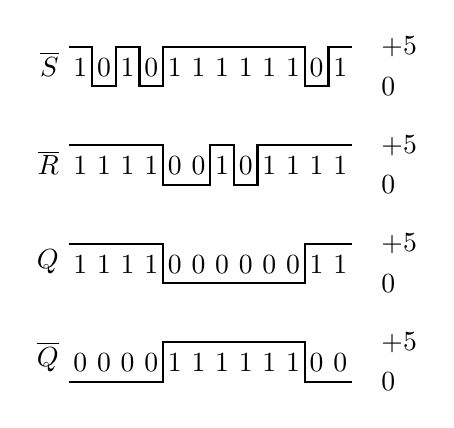
\begin{tikzpicture}
\pgfmathsetmacro{\t}{0.3}
\pgfmathsetmacro{\h}{0.5}
\pgfmathsetmacro{\kyspace}{\h+0.75}
\draw[thick](0,\h)--++(\t,0)--++(0,-\h)--++(\t,0)--++(0,\h)--++(\t,0)--++(0,-\h)--++(\t,0)--++(0,\h)--++(6*\t,0)--++(0,-\h)
--++(\t,0)--++(0,\h)--++(\t,0);
\draw[thick](0,-\kyspace+\h)--++(4*\t,0)--++(0,-\h)--++(2*\t,0)--++(0,\h)--++(\t,0)--++(0,-\h)--++(\t,0)--++(0,\h)--++(4*\t,0);
\draw[thick](0,-2*\kyspace+\h)--++(4*\t,0)--++(0,-\h)--++(6*\t,0)--++(0,\h)--++(2*\t,0);
\draw[thick](0,-3*\kyspace)--++(4*\t,0)--++(0,\h)--++(6*\t,0)--++(0,-\h)--++(2*\t,0);
\draw(0,0)node[above left]{$\overline{S}$} (0,-\kyspace)node[above left]{$\overline{R}$}
 (0,-2*\kyspace)node[above left]{$Q$} (0,-3*\kyspace)node[above left]{$\overline{Q}$};
\foreach \x/\l in {0/1,1/0,2/1,3/0,4/1,5/1,6/1,7/1,8/1,9/1,10/0,11/1}{\draw(\x*\t+\t/2,0)node[above]{$\l$};}
\foreach \x/\l in {0/1,1/1,2/1,3/1,4/0,5/0,6/1,7/0,8/1,9/1,10/1,11/1}{\draw(\x*\t+\t/2,-\kyspace)node[above]{$\l$};}
\foreach \x/\l in {0/1,1/1,2/1,3/1,4/0,5/0,6/0,7/0,8/0,9/0,10/1,11/1}{\draw(\x*\t+\t/2,-2*\kyspace)node[above]{$\l$};}
\foreach \x/\l in {0/0,1/0,2/0,3/0,4/1,5/1,6/1,7/1,8/1,9/1,10/0,11/0}{\draw(\x*\t+\t/2,-3*\kyspace)node[above]{$\l$};}
\draw(12*\t+0.25,0)node[right]{$\SI{0}{\volt}$} (12*\t+0.25,\h)node[right]{$\SI{+5}{\volt}$};
\draw(12*\t+0.25,-\kyspace)node[right]{$\SI{0}{\volt}$} (12*\t+0.25,-\kyspace+\h)node[right]{$\SI{+5}{\volt}$};
\draw(12*\t+0.25,-2*\kyspace)node[right]{$\SI{0}{\volt}$} (12*\t+0.25,-2*\kyspace+\h)node[right]{$\SI{+5}{\volt}$};
\draw(12*\t+0.25,-3*\kyspace)node[right]{$\SI{0}{\volt}$} (12*\t+0.25,-3*\kyspace+\h)node[right]{$\SI{+5}{\volt}$};
\end{tikzpicture}
\end{subfigure}
\caption{ایس آر پلٹ کار کے استعمال کا جدول اور ترسیمات۔}
\label{جدول_ترتیبی_ایس_آر_کام}
\end{figure}

شکل \حوالہ{جدول_ترتیبی_ایس_آر_کام} میں پیش جدول کی پہلے صف میں پلٹ کار بلند \عددی{(Q=1)} اور مداخل غیر فعال ہیں۔صف در صف نیچے چلتے ہوئے دیکھیں، مداخل تبدیل کرنے سے پلٹ کار کیا حال اختیار کرتا ہے۔ ( مداخل کسی خاص ترتیب سے نہیں، بلکہ پلٹ کار کی کارکردگی کی ایک مثال دیکھنے کی غرض سے تبدیل کیے گئے۔ )

مثبت منطقی نظام استعمال کرتے ہوئے، \عددی{(1)}کو \عددی{\SI{+5}{\volt}}، جبکہ \عددی{(0)} کو \عددی{\SI{0}{\volt}} سے ظاہر کیا جائے گا۔یوں مداخل ایس کی فعال صورت \عددی{\overline{S}=0} کو \عددی{\SI{0}{\volt}}، جبکہ غیر فعال صورت \عددی{\overline{S}=1} کو \عددی{\SI{+5}{\volt}} سے ظاہر کیا جائے گا۔ اسی طرح \عددی{Q=0} کو \عددی{\SI{0}{\volt}} اور \عددی{Q=1} کو \عددی{\SI{5}{\volt}} سے ظاہر کیا جائے گا۔ ایسا کرتے ہوئے شکل \حوالہ{جدول_ترتیبی_ایس_آر_کام} میں پیش جدول سے اسی شکل میں پیش ترسیمات حاصل ہوں گی، جہاں موازنہ کے لئے \عددی{\overline{Q}} بھی پیش ہے۔




\حصہ{زیادہ مداخل پلٹ کار}
پلٹ کار کے مداخل دو سے زیادہ ہو سکتے ہیں، جیسا شکل \حوالہ{شکل_ترتیبی_متمم_دو_سے_زیادہ} میں دکھایا گیا ہے۔ یہاں بلند کار مداخل کی تعداد دو ہے، جنہیں \عددی{\overline{S}_a} اور \عددی{\overline{S}_b} کہا گیا ہے، جبکہ پست کار مداخل ایک ہے۔ عام طور تینوں مداخل بلند (غیر فعال) رکھے جائیں گے۔ پلٹ کار بلند حال کرنے کی خاطر \عددی{\overline{S}_a} یا \عددی{\overline{S}_b} یا دونوں کو ایک لمحہ کے لئے پست (فعال) کیا جائے گا، جبکہ پلٹ کار پست حال کرنے کی خاطر \عددی{\overline{R}} ایک لمحہ کے لئے فعال کیا جائے گا۔ حال دوڑ سے بچنے کے لئے ضروری ہے کہ \عددی{\overline{R}} کے ساتھ باقی دو مداخل میں سے کوئی ایک (یا دونوں) اکٹھے فعال نہ کیا جائے۔


\begin{figure}
\centering
\begin{subfigure}{0.45\textwidth}
\centering
\begin{tikzpicture}
\pgfmathsetmacro{\kxsep}{2.5}
\pgfmathsetmacro{\kysep}{2}
\pgfmathsetmacro{\kpin}{0.5}
\draw(0,0)node[nand port,scale=1,number inputs=2](u1){};
\draw(0,\kysep)node[nand port,scale=1,number inputs=3](u2){};
\draw(u1.out)--++(\kpin,0)node[right]{$\overline{Q}$};
\draw(u2.out)--++(\kpin,0)node[right]{$Q$};
\draw(u1.out)--++(0,\kpin)coordinate(aa) (u2.out)--++(0,-\kpin)coordinate(bb);
\draw(u1.in 1)--++(0,\kpin)coordinate(cc) (u2.in 3)--++(0,-\kpin)coordinate(dd);
\draw(bb)--(cc) (aa)--(dd);
\draw(u1.in 2)--++(-\kpin,0)node[left]{$\overline{R}$};
\draw(u2.in 1)--++(-\kpin,0)node[left,yshift=0.25em]{$\overline{S}_a$};
\draw(u2.in 2)--++(-\kpin,0)node[left,yshift=-0.25em]{$\overline{S}_b$};
\end{tikzpicture}
\end{subfigure}\hfill
\begin{subfigure}{0.45\textwidth}
\centering
\begin{otherlanguage}{english}
\begin{tabular}{CCC|CC}
\toprule
\overline{S}_a&\overline{S}_b&\overline{R}&Q_{n+1}&\overline{Q}_{n+1}\\
\midrule
0&0&0&?&?\\
0&0&1&1&0\\
0&1&0&?&?\\
0&1&1&1&0\\
1&0&0&?&?\\
1&0&1&1&0\\
1&1&0&0&1\\
1&1&1&Q_n&\overline{Q}_n\\
\bottomrule
\end{tabular}
\end{otherlanguage}
\end{subfigure}
\caption{زیادہ مداخل ایس آر پلٹ کار}
\label{شکل_ترتیبی_متمم_دو_سے_زیادہ}
\end{figure}


\حصہ{قابل مجاز و معذور پلٹ کار}
 شکل \حوالہ{جدول_ترتیبی_ایس_آر_کام} کی ترسیمات سے واضح ہے، مداخل تبدیل کرتے ہی پلٹ کار نیا حال اختیار کرتا ہے۔اس حصہ میں ایسی پلٹ کار پر غور کیا جائے گا جس کے مداخل کو پلٹ کار کے حال پر اثر انداز ہونے سے روکا جا سکتا ہو۔ شکل\حوالہ{شکل_ترتیبی_قابل_مجاز}الف پر غور کریں جہاں دو متمم ضرب گیٹ کے اضافہ سے قابل قابو پلٹ کار حاصل کیا گیا، جس کے (بلند فعال) مداخل \عددی{S} اور \عددی{R} ہیں، جنہیں عام طور غیر فعال (پست) رکھا جاتا ہے۔پلٹ کار کی علامت شکل-ب بھی پیش ہے۔
 
 اضافی گیٹ کے مخارج کو \عددی{\overline{S}_c} اور \عددی{\overline{R}_c} کہا گیا، جبکہ گیٹوں کو قابو کار اشارہ \عددی{C} فراہم کیا گیا۔ مجاز و معذور بنانے والا قابو کار اشارہ \عددی{C} پست (معذور) کرنے سے \عددی{S} اور \عددی{R} مداخل معذور ہوتے ہیں، \عددی{\overline{S}_c} اور \عددی{\overline{R}_c} بلند رہتے ہیں، اور پلٹ کار اپنا حال برقرار رکھتی ہے۔ قابو کار اشارہ بلند (مجاز) کرنے سے پلٹ کار کے مداخل \عددی{S} اور \عددی{R} مجاز ہو کر پلٹ کار کے حال پر اثر انداز ہوتے ہیں۔ 
 
 شکل-ج میں مجاز و معذور قابو کار اشارہ \عددی{C} کی کارکردگی واضح کی گئی۔ جب تک یہ اشارہ پست (معذور) رہے، \عددی{\overline{S}_c} اور \عددی{\overline{R}_c} بلند ہیں۔ اشارہ \عددی{C} بلند کرنے کے بعد \عددی{S} اور \عددی{R} پلٹ کار کا حال تبدیل کرنے کے قابل ہیں۔ یہ پلٹ کار \موٹا{ مجاز و معذور بلند فعال مداخل ایس آر پلٹ کار} کہلاتا ہے۔
 
 
\begin{figure}
\centering
\begin{subfigure}{0.55\textwidth}
\centering
\begin{tikzpicture}
\pgfmathsetmacro{\kxsep}{2.5}
\pgfmathsetmacro{\kysep}{2}
\pgfmathsetmacro{\kpin}{0.5}
\draw(0,0)node[nand port,scale=1,number inputs=2](u1){};
\draw(0,\kysep)node[nand port,scale=1,number inputs=2](u2){};
\draw(u1.out)--++(\kpin,0)node[right]{$\overline{Q}$};
\draw(u2.out)--++(\kpin,0)node[right]{$Q$};
\draw(u1.out)--++(0,\kpin)coordinate(aa) (u2.out)--++(0,-\kpin)coordinate(bb);
\draw(u1.in 1)--++(0,\kpin)coordinate(cc) (u2.in 2)--++(0,-\kpin)coordinate(dd);
\draw(bb)--(cc) (aa)--(dd);
\draw(u1.in 2)--++(-\kpin,0)node[above]{$\overline{R}_c$}node[nand port,scale=1,number inputs=2,anchor=out](u3){};
\draw(u2.in 1)--++(-\kpin,0)node[above]{$\overline{S}_c$}node[nand port,scale=1,number inputs=2,anchor=out](u4){};
\draw(u3.in 2)--++(-\kpin,0)node[left]{$R$};
\draw(u4.in 1)--++(-\kpin,0)node[left]{$S$};
\draw(u3.in 1)--(u4.in 2)coordinate[pos=0.5](cc) (cc)--++(-\kpin,0)node[left]{$C$};
\end{tikzpicture}
\caption{}
\end{subfigure}\hfill
\begin{subfigure}{0.35\textwidth}
\centering
\begin{tikzpicture}
\kSRFF[u1]{0}{0}
\end{tikzpicture}
\caption{}
\end{subfigure}
\begin{subfigure}{1\textwidth}
\centering
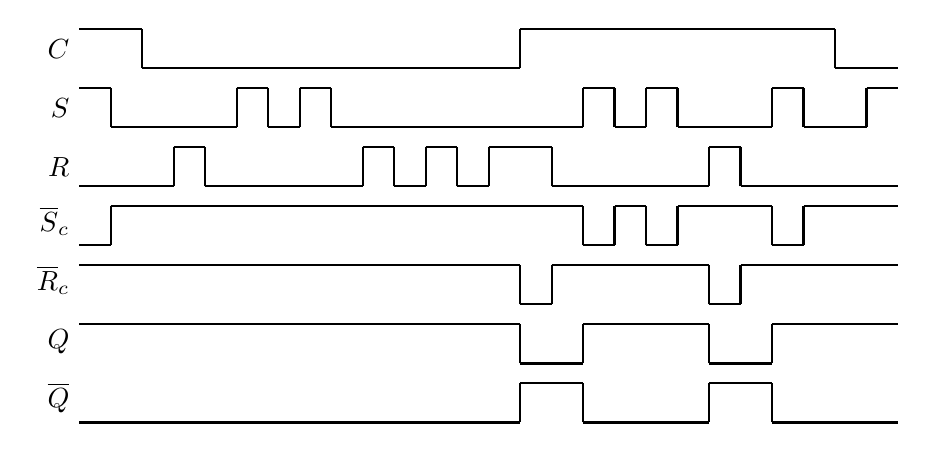
\begin{tikzpicture}
\pgfmathsetmacro{\t}{0.4}
\pgfmathsetmacro{\h}{0.5}
\pgfmathsetmacro{\kysep}{\h+0.25}
\foreach \xha/\xhb in {0/2,14/24}{\draw[thick](\xha*\t,\h)--(\xhb*\t,\h);} 
\foreach \xla/\xlb in {2/14,24/26}{\draw[thick](\xla*\t,0)--(\xlb*\t,0);} 
\foreach \xv in {2,14,24}{\draw[thick](\xv*\t,0)--++(0,\h);}
\draw(0,-0*\kysep)node[above left]{$C$};
\foreach \xha/\xhb in {0/1,5/6,7/8,16/17,18/19,22/23,25/26}{\draw[thick](\xha*\t,-1*\kysep+\h)--(\xhb*\t,-1*\kysep+\h);} 
\foreach \xla/\xlb in {1/5,6/7,8/16,17/18,19/22,23/25}{\draw[thick](\xla*\t,-1*\kysep)--(\xlb*\t,-1*\kysep);} 
\foreach \xv in {1,5,6,7,8,16,17,18,19,22,23,25}{\draw[thick](\xv*\t,-1*\kysep)--++(0,\h);}
\draw(0,-1*\kysep)node[above left]{$S$};
\foreach \xha/\xhb in {3/4,9/10,11/12,13/15,20/21}{\draw[thick](\xha*\t,-2*\kysep+\h)--(\xhb*\t,-2*\kysep+\h);}
\foreach \xla/\xlb in {0/3,4/9,10/11,12/13,15/20,21/26}{\draw[thick](\xla*\t,-2*\kysep)--(\xlb*\t,-2*\kysep);}
\foreach \xv in {3,4,9,10,11,12,13,15,20,21}{\draw[thick](\xv*\t,-2*\kysep)--++(0,\h);}
\draw(0,-2*\kysep)node[above left]{$R$};
\foreach \xha/\xhb in {1/16,17/18,19/22,23/26}{\draw[thick](\xha*\t,-3*\kysep+\h)--(\xhb*\t,-3*\kysep+\h);}
\foreach \xla/\xlb in {0/1,16/17,18/19,22/23}{\draw[thick](\xla*\t,-3*\kysep)--(\xlb*\t,-3*\kysep);}
\foreach \xv in {1,16,17,18,19,22,23}{\draw[thick](\xv*\t,-3*\kysep)--++(0,\h);}
\draw(0,-3*\kysep)node[above left]{$\overline{S}_c$};
\foreach \xha/\xhb in {0/14,15/20,21/26}{\draw[thick](\xha*\t,-4*\kysep+\h)--(\xhb*\t,-4*\kysep+\h);}
\foreach \xla/\xlb in {14/15,20/21}{\draw[thick](\xla*\t,-4*\kysep)--(\xlb*\t,-4*\kysep);}
\foreach \xv in {14,15,20,21}{\draw[thick](\xv*\t,-4*\kysep)--++(0,\h);}
\draw(0,-4*\kysep)node[above left]{$\overline{R}_c$};
\foreach \xha/\xhb in {0/14,16/20,22/26}{\draw[thick](\xha*\t,-5*\kysep+\h)--(\xhb*\t,-5*\kysep+\h);}
\foreach \xla/\xlb in {14/16,20/22}{\draw[thick](\xla*\t,-5*\kysep)--(\xlb*\t,-5*\kysep);}
\foreach \xv in {14,16,20,22}{\draw[thick](\xv*\t,-5*\kysep)--++(0,\h);}
\draw(0,-5*\kysep)node[above left]{$Q$};
\foreach \xha/\xhb in {14/16,20/22}{\draw[thick](\xha*\t,-6*\kysep+\h)--(\xhb*\t,-6*\kysep+\h);}
\foreach \xla/\xlb in {0/14,16/20,22/26} {\draw[thick](\xla*\t,-6*\kysep)--(\xlb*\t,-6*\kysep);}
\foreach \xv in {14,16,20,22}{\draw[thick](\xv*\t,-6*\kysep)--++(0,\h);}
\draw(0,-6*\kysep)node[above left]{$\overline{Q}$};
\end{tikzpicture}
\caption{}
\end{subfigure}
\caption{مجاز و معذور بلند فعال مداخل ایس آر پلٹ کار}
\label{شکل_ترتیبی_قابل_مجاز}
\end{figure}
	
بعض اوقات، پلٹ کار کے عمومی مداخل استعمال کیے بغیر، ہم پلٹ کار کا حال خود تعین کرنا چاہتے ہیں۔عموماً، پلٹ کار کا ابتدائی حال منتخب کرنے کے لئے ایسا کرنا درکار ہو گا۔شکل \حوالہ{شکل_ترتیبی_زبردستی_بلند_قابل_مجاز} میں دو مزید مداخل، \عددی{\overline{\text{اٹھ}}} اور \عددی{\overline{\text{بیٹھ}}}، مہیا کئے گئے ہیں، جنہیں پست کر کے پلٹ کار کو بالترتیب زبردستی بلند اور پست کیا جا سکتا ہے۔
\begin{figure}
\centering
\begin{subfigure}{0.55\textwidth}
\centering
\begin{tikzpicture}
\pgfmathsetmacro{\kxsep}{2.5}
\pgfmathsetmacro{\kysep}{2}
\pgfmathsetmacro{\kpin}{0.5}
\draw(0,0)node[nand port,scale=1,number inputs=3](u1){};
\draw(0,\kysep)node[nand port,scale=1,number inputs=3](u2){};
\draw(u1.out)--++(\kpin,0)node[right]{$\overline{Q}$};
\draw(u2.out)--++(\kpin,0)node[right]{$Q$};
\draw(u1.out)--++(0,\kpin)coordinate(aa) (u2.out)--++(0,-\kpin)coordinate(bb);
\draw(u1.in 1)--++(0,\kpin/2)coordinate(cc) (u2.in 3)--++(0,-\kpin/2)coordinate(dd);
\draw(bb)--(cc) (aa)--(dd);
\draw(u1.in 2)--++(-\kpin,0)node[nand port,scale=1,number inputs=2,anchor=out](u3){};
\draw(u2.in 2)--++(-\kpin,0)node[nand port,scale=1,number inputs=2,anchor=out](u4){};
\draw(u3.in 2)--++(-\kpin,0)node[left]{$R$};
\draw(u4.in 1)--++(-\kpin,0)node[left]{$S$};
\draw(u3.in 1)--(u4.in 2)coordinate[pos=0.5](cc) (cc)--++(-\kpin,0)node[left]{$C$};
\draw(u1.in 3)--++(0,-1.5*\kpin)--++(-2*\kpin,0)node[left]{$\overline{\text{\RL{بیٹھ}}}$};
\draw(u2.in 1)--++(0,1.5*\kpin)--++(-2*\kpin,0)node[left]{$\overline{\text{\RL{اٹھ}}}$};
\end{tikzpicture}
\end{subfigure}\hfill
\begin{subfigure}{0.35\textwidth}
\centering
\begin{tikzpicture}
\pgfmathsetmacro{\kshPa}{0.50}
\kSRFF[u1]{0}{0}
\draw(u1pbu)--++(0,\kshPa)node[above]{$\overline{\text{\RL{اٹھ}}}$};
\draw(u1pbd)--++(0,-\kshPa)node[below]{$\overline{\text{\RL{بیٹھ}}}$};
\draw(u1pnu)node[ocirc]{} (u1pnd)node[ocirc]{};
\end{tikzpicture}
\end{subfigure}
\caption{اٹھ بیٹھ صلاحیت پلٹ کار}
\label{شکل_ترتیبی_زبردستی_بلند_قابل_مجاز}
\end{figure}


\حصہ{آقا غلام پلٹ کار} 	
گزشتہ حصہ میں مجاز و معذور بلند فعال مداخل ایس آر پلٹ کار پر غور کیا گیا۔شکل \حوالہ{شکل_ترتیبی_آقا_غلام} میں ایسے دو پلٹ کار ( پہلا آقا اور دوسرا غلام کہلاتا ہے) اور ایک نفی گیٹ سے \اصطلاح{آقا غلام پلٹ کار}\فرہنگ{پلٹ کار!آقا غلام}\حاشیہب{master slave flip flop}\فرہنگ{flip flop!master slave} تشکیل دیا گیا۔آقا کے مخارج، غلام کے مداخل ہیں۔مزید \عددی{C} پر اشارہ \اصطلاح{ساعت}\فرہنگ{ساعت}\حاشیہب{clock}\فرہنگ{clock} مہیا کیا گیا ہے۔
\begin{figure}
\centering
\begin{subfigure}{1\textwidth}
\centering
\begin{tikzpicture}
\pgfmathsetmacro{\kshPa}{0.50}
\pgfmathsetmacro{\kshXX}{2.5}
\pgfmathsetmacro{\kshYY}{0.75}
\kSRFF[u1]{0}{0}
\kSRFF[u2]{\kshXX}{0}
\draw(u1p6)--(u2p1) (u1p4)--(u2p3);
\draw(u1p1)--++(-\kshPa,0)node[left]{$S$} (u1p3)--++(-\kshPa,0)node[left]{$R$};
\draw(u2p6)node[right]{$Q$} (u2p4)node[right]{$\overline{Q}$};
\draw(u1p2)--++(-\kshPa,0)node[left]{$C$};
\draw(0,-\kshYY)node[not port,scale=0.7,anchor=in](u3){};
\draw(u1p2)|-(u3.in 1) (u3.out)-|(u2p2);
\draw(u1p6)node[above]{$Q_a$} (u1p4)node[above]{$\overline{Q}_a$};
\draw(u1-north)node[above]{\text{\RL{آقا}}};
\draw(u2-north)node[above]{\text{\RL{غلام}}};
\end{tikzpicture}
\caption{}
\end{subfigure}
\begin{subfigure}{1\textwidth}
\centering
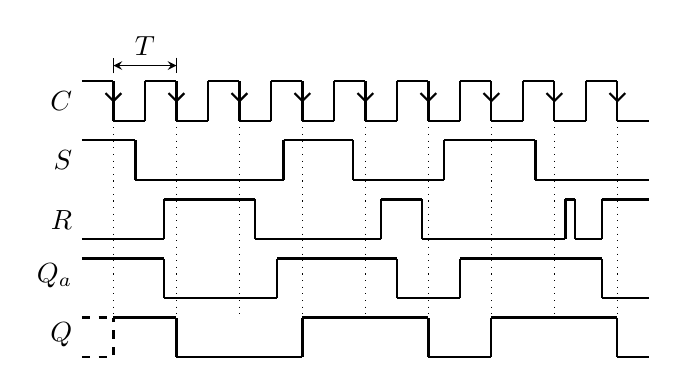
\begin{tikzpicture}
\pgfmathsetmacro{\t}{0.4}
\pgfmathsetmacro{\h}{0.5}
\pgfmathsetmacro{\dx}{0.1}
\pgfmathsetmacro{\dy}{0.1}
\pgfmathsetmacro{\kysep}{\h+0.25}
\foreach \xha/\xhb in {0/1,2/3,4/5,6/7,8/9,10/11,12/13,14/15,16/17}{\draw[thick](\xha*\t,\h)--(\xhb*\t,\h);} 
\foreach \xla/\xlb in {1/2,3/4,5/6,7/8,9/10,11/12,13/14,15/16,17/18}{\draw[thick](\xla*\t,0)--(\xlb*\t,0);} 
\foreach \xv in {1,2,3,4,5,6,7,8,9,10,11,12,13,14,15,16,17}{\draw[thick](\xv*\t,0)--++(0,\h);}
\foreach \xv in {1,3,5,7,9,11,13,15,17}{\draw[thick](\xv*\t,\h/2)--++(\dx,\dy) (\xv*\t,\h/2)--++(-\dx,\dy);}
\draw(0,-0*\kysep)node[above left]{$C$};
\draw(\t,\h)++(0,0.1)--++(0,0.2)coordinate[pos=0.5](aa)++(2*\t,0)--++(0,-0.2);
\draw[stealth-stealth] (aa)--++(2*\t,0)node[pos=0.5,above]{$T$};
\foreach \xha/\xhb in {0/1.7,6.4/8.6,11.5/14.4}{\draw[thick](\xha*\t,-1*\kysep+\h)--(\xhb*\t,-1*\kysep+\h);} 
\foreach \xla/\xlb in {1.7/6.4,8.6/11.5,14.4/18}{\draw[thick](\xla*\t,-1*\kysep)--(\xlb*\t,-1*\kysep);} 
\foreach \xv in {1.7,6.4,8.6,11.5,14.4}{\draw[thick](\xv*\t,-1*\kysep)--++(0,\h);}
\draw(0,-1*\kysep)node[above left]{$S$};
\foreach \xha/\xhb in {2.6/5.5,9.5/10.8,15.35/15.65,16.5/18}{\draw[thick](\xha*\t,-2*\kysep+\h)--(\xhb*\t,-2*\kysep+\h);}
\foreach \xla/\xlb in {0/2.6,5.5/9.5,10.8/15.35,15.65/16.5}{\draw[thick](\xla*\t,-2*\kysep)--(\xlb*\t,-2*\kysep);}
\foreach \xv in {2.6,5.5,9.5,10.8,15.35,15.65,16.5}{\draw[thick](\xv*\t,-2*\kysep)--++(0,\h);}
\draw(0,-2*\kysep)node[above left]{$R$};
\foreach \xha/\xhb in {0/2.6,6.2/10,12/16.5}{\draw[thick](\xha*\t,-3*\kysep+\h)--(\xhb*\t,-3*\kysep+\h);}
\foreach \xla/\xlb in {2.6/6.2,10/12,16.5/18}{\draw[thick](\xla*\t,-3*\kysep)--(\xlb*\t,-3*\kysep);}
\foreach \xv in {2.6,6.2,10,12,16.5}{\draw[thick](\xv*\t,-3*\kysep)--++(0,\h);}
\draw(0,-3*\kysep)node[above left]{$Q_a$};
\foreach \xha/\xhb in {1/3,7/11,13/17}{\draw[thick](\xha*\t,-4*\kysep+\h)--(\xhb*\t,-4*\kysep+\h);}
\foreach \xla/\xlb in {3/7,11/13,17/18}{\draw[thick](\xla*\t,-4*\kysep)--(\xlb*\t,-4*\kysep);}
\foreach \xv in {3,7,11,13,17}{\draw[thick](\xv*\t,-4*\kysep)--++(0,\h);}
\draw(0,-4*\kysep)node[above left]{$Q$};
\draw[dashed,thick](0,-4*\kysep)--++(\t,0)--++(0,\h) (0,-4*\kysep+\h)--++(\t,0);
\foreach \x in {1,3,5,7,9,11,13,15,17}{\draw[dotted] (\x*\t,0)--++(0,-4*\kysep+\h);}
\end{tikzpicture}
\caption{}
\end{subfigure}
\caption{ساعت کے کنارہ اترائی پر عمل کار آقا غلام پلٹ کار}
\label{شکل_ترتیبی_آقا_غلام}
\end{figure}



 جتنی دیر ساعت \عددی{(C)} بلند رہے، آقا کے مداخل مجاز، لہٰذا مخارج \عددی{Q_a} اور \عددی{\overline{Q}_a} قابل تبدیل ہوں گے۔ غلام کو \عددی{C} کا متمم \عددی{\overline{C}} مجاز و معذور بناتا ہے، لہٰذا جتنی دیر آقا مجاز ہو، غلام معذور (لہٰذا برقرار حال) ہو گا۔
 
جس لمحہ ساعت پست ہو، آقا اسی لمحہ کے حال میں رہ جائے گا، اور غلام مجاز ہو کر فوراً آقا کے مخارج کے مطابق حال اختیار کر لے گا۔یوں، غلام ہر وقت آقا کی پیروی کرتا ہے۔جتنی دیر ساعت پست رہے، \عددی{Q_a} اور \عددی{\overline{Q}_a} تبدیل نہیں ہو سکتے، لہٰذا غلام حال تبدیل نہیں کرے گا۔


 آپ دیکھ سکتے ہیں، غلام پلٹ کار صرف اور صرف ساعت \عددی{(C)} کے کنارہ اترائی پر حال تبدیل کرتا ہے، جس کی وجہ سے یہ \اصطلاح{کنارہ اترائی پر عمل کار آقا غلام پلٹ کار}\فرہنگ{آقا غلام!کنارہ اترائی پر عمل کار}\حاشیہب{negative edge triggered Master Slave flip flop}\فرہنگ{master slave!negative edge triggered} کہلاتا ہے۔ ساعت کے کنارہ اترائی پر تیر کا نشان اس حقیقت کو ظاہر کرتا ہے۔ساعت کا کنارہ (اترائی)، پلٹ کار کی \اصطلاح{لبلبی}\فرہنگ{لبلبی}\حاشیہب{trigger}\فرہنگ{trigger} ہے، جسے پست کرنے سے، پلٹ کار داخلی اشارے کا عکس لیتا ہے۔

 پلٹ کار کو پہلی مرتبہ برقی طاقت فراہم کرنے سے، حال دوڑ پیدا ہو گی جس کے اختتام پر پلٹ کار بلند یا پست ہو گا۔ شکل میں پہلے کنارہ اترائی سے قبل \عددی{Q} مبہم دکھایا گیا ہے (سایہ دار حصہ) ، جو اس حقیقت کو ظاہر کرتا ہے۔ساعت کے اول کنارہ اترائی پر فعال \عددی{S} کے تحت آقا غلام پلٹ کار یقینی طور پر بلند حال اختیار کرتا ہے۔ (شکل \حوالہ{شکل_ترتیبی_زبردستی_بلند_قابل_مجاز} میں اٹھ بیٹھ قابو اشارات اس طرح مبہم صورت سے نمٹنے کے لئے ہیں۔)
 
شکل \حوالہ{شکل_ترتیبی_آقا_غلام} میں ساعت کے آٹھویں کنارہ اترائی کے بعد پست ساعت کے دوران \عددی{R} بلند ہو کر واپس پست ہوتا ہے، جو آقا غلام پلٹ کار کو پست کرنے میں ہرگز کامیاب نہیں ہو گا۔ پلٹ کار کو بلند یا پست کرنے کے لئے، ضروری ہے کہ داخلی اشارات \عددی{S} اور \عددی{R} کسی مخصوص دورانیے سے زیادہ وقت کے لئے فعال ہوں۔ داخلی اشارہ اس صورت کردار ادا کرتا ہے، جب بلند ساعت اس کا عکس محفوظ کر لے۔ ساعت کے پست دورانیہ \عددی{t_L} (شکل \حوالہ{شکل_ترتیبی_ساعت_تفصیل}) سے زیادہ دیر فعال رہنے والا مداخل اشارہ ، ساعت کے کنارہ اترائی کے فوراً بعد فعال ہونے کی صورت میں بھی ساعت کی اگلی بلندی تک فعال رہے گا، لہٰذا آقا غلام پلٹ کار اس پر ضرور عمل کرے گا۔ البتہ، ایسی صورت میں عین ممکن ہے، کنارہ اترائی پر کوئی مداخل فعال نہ ہو (شکل \حوالہ{شکل_ترتیبی_آقا_غلام} میں چھٹا کنارہ اترائی دیکھیں)، لہٰذا، عین کنارہ اترائی کے لمحہ موجود مداخل کا حال محفوظ کرنے کے لئے ضروری ہے کہ مداخل کم از کم ایک دوری عرصہ \عددی{(T)} دورانیے کے لئے فعال رہے (تسلی کر لیں، اگر یقین نہیں)۔ حصہ \حوالہ{حصہ_ترتیبی_حقیقی_ڈی_پلٹ} میں ایسی پلٹ کار پیش کیا جائے گا، جس کے مداخل پر کم از کم ایک دوری عرصہ فعال رہنے کی شرط مسلط نہیں۔

جدول \حوالہ{جدول_ترتیبی_آقا_غلام} میں کنارہ اترائی پر عمل کار آقا غلام پلٹ کار پیش ہے، جہاں ساعت کے کنارہ اترائی پر پلٹ کار (نیا) حال اختیار کرتا ہے۔بلند اور پست ساعت کے دوران، پلٹ کار حال برقرار رکھتا ہے۔
\begin{table}
\caption{کنارہ اترائی پر عمل کار آقا غلام پلٹ کار}
\label{جدول_ترتیبی_آقا_غلام}
\centering
\begin{otherlanguage}{english}
\begin{tabular}{CCC|CC}
\toprule
C&S&R&Q_{n+1}&\overline{Q}_{n+1}\\
\midrule
0&x&x&Q_n&\overline{Q}_n\\
1&x&x&Q_n&\overline{Q}_n\\
\downarrow&0&0&Q_n&\overline{Q}_n\\
\downarrow&0&1&0&1\\
\downarrow&1&0&1&0\\
\downarrow&1&1&?&?\\
\bottomrule
\end{tabular}
\end{otherlanguage}
\end{table}
 

\begin{figure}
\centering
\begin{subfigure}{0.80\textwidth}
\centering
\begin{tikzpicture}
\pgfmathsetmacro{\kxsep}{2.5}
\pgfmathsetmacro{\kysep}{2}
\pgfmathsetmacro{\kpin}{0.5}
\draw(0,0)node[nand port,scale=1,number inputs=3](u1){};
\draw(0,\kysep)node[nand port,scale=1,number inputs=3](u2){};
\draw(u1.out)--++(\kpin,0)node[right]{$\overline{Q}$};
\draw(u2.out)--++(\kpin,0)node[right]{$Q$};
\draw(u1.out)--++(0,\kpin)coordinate(aa) (u2.out)--++(0,-\kpin)coordinate(bb);
\draw(u1.in 1)--++(0,\kpin/2)coordinate(cc) (u2.in 3)--++(0,-\kpin/2)coordinate(dd);
\draw(bb)--(cc) (aa)--(dd);
\draw(u1.in 2)node[nand port,scale=1,number inputs=2,anchor=out](u3){};
\draw(u2.in 2)node[nand port,scale=1,number inputs=2,anchor=out](u4){};
\draw(u3.in 2)--++(-\kpin,0)node[nand port, scale=1,number inputs=3,anchor=out](u5){};
\draw(u4.in 1)--++(-\kpin,0)node[nand port, scale=1,number inputs=3,anchor=out](u6){};
\draw(u5.out)--++(0,\kpin)coordinate(aa) (u6.out)--++(0,-\kpin)coordinate(bb);
\draw(u5.in 1)--++(0,\kpin/2)coordinate(cc) (u6.in 3)--++(0,-\kpin/2)coordinate(dd);
\draw(bb)--(cc) (aa)--(dd);
\draw(u5.in 2)node[nand port,scale=1,number inputs=2,anchor=out](u7){};
\draw(u6.in 2)node[nand port,scale=1,number inputs=2,anchor=out](u8){};
\draw($(u7.in 1)!0.5!(u8.in 2)$) node[not port,scale=0.8,anchor=in](u9){};
\draw(u3.in 1)--(u4.in 2)coordinate[pos=0.5](cc) (cc)--(u9.out);
\draw(u7.in 2)--++(-\kpin,0)node[left]{$R$};
\draw(u8.in 1)--++(-\kpin,0)node[left]{$S$};
\draw(u7.in 1)--(u8.in 2) (u9.in) to [short,*-]++(-\kpin,0)node[left]{$C$};
\draw(u1.in 3)--++(0,-1.5*\kpin)coordinate(ksit)--($(u7.in 1)!(ksit)!(u8.in 1)$)coordinate(ksitL)
node[left]{$\overline{\text{\RL{بیٹھ}}}$};
\draw(u2.in 1)--++(0,1.5*\kpin)coordinate(kstand)--($(u7.in 1)!(kstand)!(u8.in 1)$)coordinate(kstandL)
node[left]{$\overline{\text{\RL{اٹھ}}}$};
\draw(u5.in 3)--($(ksit)!(u5.in 3)!(ksitL)$);
\draw(u6.in 1)--($(kstand)!(u6.in 1)!(kstandL)$);
\end{tikzpicture}
\end{subfigure}\hfill
\begin{subfigure}{0.20\textwidth}
\centering
\begin{tikzpicture}
\pgfmathsetmacro{\kshPa}{0.4}
\kSRFF[u1]{0}{0}
\draw(u1pbu)--++(0,\kshPa)node[above]{$\overline{\text{اٹھ}}$};
\draw(u1pnu)node[ocirc]{};
\draw(u1pbd)--++(0,-\kshPa)node[below]{$\overline{\text{بیٹھ}}$};
\draw(u1pnd)node[ocirc]{};
\draw(u1pn2)node[ocirc]{};
\end{tikzpicture}
\end{subfigure}
\caption{اٹھ بیٹھ صلاحیت رکھنے اور منفی کنارے پر عمل کرنے والا آقا غلام پلٹ کار}
\label{شکل_ترتیبی_اٹھ_بیٹھ_آقا_غلام}
\end{figure}

بعض اوقات، پلٹ کار کا حال، کنارہ ساعت کا انتظار کیے بغیر، تبدیل کرنا درکار ہو گا۔شکل \حوالہ{شکل_ترتیبی_اٹھ_بیٹھ_آقا_غلام} میں (درکار مقامات پر تین مداخل متمم ضرب گیٹ استعمال کرتے ہوئے) آقا غلام پلٹ کار میں پست فعال مداخل \عددی{\overline{\text{اٹھ}}} اور \عددی{\overline{\text{بیٹھ}}} کا اضافہ کر کے ایسی پلٹ کار تشکیل دیا گیا ہے۔ (برقی تاروں کی تعداد بہت بڑھ گئی ہے۔ بہتر ہو گا صفحہ \حوالہصفحہ{شکل_بوولین_برقی_تار_جوڑ} پر شکل \حوالہ{شکل_بوولین_برقی_تار_جوڑ} ایک مرتبہ دوبارہ دیکھیں۔) عام طور انہیں غیر فعال رکھا جائے گا، البتہ، جب ضرورت پیش آئے، انہیں استعمال کرتے ہوئے، ساعت کے کنارہ اترائی کا انتظار کیے بغیر، پلٹ کار کا حال مرضی کے مطابق منتخب کیا جا سکے گا۔

شکل میں \موٹا{منفی کنارے پر عمل کرنے، اور اٹھ بیٹھ صلاحیت کے ، آقا غلام پلٹ کار} کی علامت بھی پیش ہے، جہاں ساعت \عددی{(C)} پر گول دائرہ \موٹا{منفی}، اور تکون \موٹا{کنارے} کو ظاہر کرتا ہے ۔یوں اس سے مراد \قول{ساعت کے منفی کنارے پر عمل پیرا ہونا} لیا جائے گا۔


\حصہ{ ڈی پلٹ کار} 
\جزوحصہ{آقا غلام پلٹ کار سے حاصل کردہ ڈی پلٹ کار}
آقا غلام پلٹ کار کے ساتھ نفی گیٹ منسلک کرکے \اصطلاح{ڈی پلٹ کار}\فرہنگ{پلٹ کار!ڈی}\حاشیہب{D FF}\فرہنگ{FF!D} حاصل کیا جاتا ہے، جو شکل \حوالہ{شکل_ترتیبی_ڈی_پلٹ} میں پیش ہے۔ پلٹ کار کی علامت میں \عددی{C} واضح طور نہیں لکھا گیا، چونکہ علامت پر داخلی جانب گول دائرہ اور تکون ساعت کے منفی کنارہ کو ظاہر کرتے ہیں (مثبت کنارہ، صرف تکون سے ظاہر کیا جاتا ہے)۔ مداخل \عددی{D} پر کم از کم ایک دوری عرصہ \عددی{(T)} بلند یا پست رہنے کی شرط مسلط ہے۔

 پلٹ کار کی کارکردگی کا جدول بھی شکل \حوالہ{شکل_ترتیبی_ڈی_پلٹ} میں پیش ہے،جس کے تحت، بلند یا پست ساعت کے دوران، مداخل \عددی{D}، پلٹ کار کے حال پر اثر انداز نہیں ہو گا۔ پلٹ کار (صرف) ساعت کے کنارہ اترائی پر \عددی{D} دیکھ کر (نیا) حال اختیار کرتا ہے۔ یوں اس کا نام \اصطلاح{کنارہ اترائی پر عمل کار ڈی پلٹ کار}\فرہنگ{پلٹ کار!ڈی، کنارہ اترائی لبلبی}\حاشیہب{negative edge triggered, D flip flop}\فرہنگ{flip flop!D, negative edge} ہو گا۔ ساعت کو نفی گیٹ سے گزار کر \اصطلاح{کنارہ چڑھائی پر عمل کار ڈی پلٹ کار}\فرہنگ{پلٹ کار!ڈی، کنارہ چڑھائی لبلبی}\حاشیہب{positive edge triggered, D flip flop}\فرہنگ{flip flop!D, positive edge} حاصل ہو گا۔

\begin{figure}
\centering
\begin{subfigure}{0.40\textwidth}
\centering
\begin{tikzpicture}
\pgfmathsetmacro{\kshPa}{0.4}
\kSRFF[u1]{0}{0}
\draw(u1pbu)--++(0,\kshPa)node[above]{$\overline{\text{اٹھ}}$};
\draw(u1pnu)node[ocirc]{};
\draw(u1pbd)--++(0,-\kshPa)node[below]{$\overline{\text{بیٹھ}}$};
\draw(u1pnd)node[ocirc]{};
\draw(u1pn2)node[ocirc]{};
\draw(u1p3)node[not port,scale=1,number inputs=1,anchor=out](u2){} (u2.in)|-coordinate(ss)(u1p1) (ss)--++(-\kshPa,0)coordinate(aal)node[left]{$D$};
\draw(u1p2)node[left]{$C$};
\end{tikzpicture}
\end{subfigure}\hfill
\begin{subfigure}{0.35\textwidth}
\centering
\begin{tikzpicture}
\pgfmathsetmacro{\kshPa}{0.4}
\kDFF[u1]{0}{0}
\draw(u1pbu)--++(0,\kshPa)node[above]{$\overline{\text{اٹھ}}$};
\draw(u1pnu)node[ocirc]{};
\draw(u1pbd)--++(0,-\kshPa)node[below]{$\overline{\text{بیٹھ}}$};
\draw(u1pnd)node[ocirc]{};
\draw(u1pn2)node[ocirc]{};
\end{tikzpicture}
\end{subfigure}\hfill
\begin{subfigure}{0.25\textwidth}
\centering
\begin{otherlanguage}{english}
\begin{tabular}{CC|C}
\toprule
C&D&Q_{n+1}\\
\midrule
0&x&Q_n\\
1&x&Q_n\\
\downarrow&0&0\\
\downarrow&1&1\\
\bottomrule
\end{tabular}
\end{otherlanguage}
\end{subfigure}
\caption{آقا غلام سے حاصل ڈی پلٹ کار}
\label{شکل_ترتیبی_ڈی_پلٹ}
\end{figure}



 شکل \حوالہ{شکل_ترتیبی_ڈی_پلٹ_اوقات} میں ڈی پلٹ کار کی کارکردگی کی مثال پیش ہے۔ آقا غلام پلٹ کار کے \عددی{R} مداخل سے چھٹکارا حاصل کرنے کی بدولت، ڈی پلٹ کار کسی صورت \قول{حال دوڑ} سے دو چار نہیں ہو گا۔ساعت کے اول کنارہ اترائی سے قبل، پلٹ کار کا حال مبہم ہے، جس کو سیاہ کر کے (بلند و پست دونوں) دکھایا گیا ہے۔
 \begin{figure}
 \centering
 \begin{otherlanguage}{english}
 \begin{tikztimingtable}[%
timing/.style={x=4ex,y=3ex},
timing/rowdist=5ex,
every node/.style={inner sep=0,outer sep=0},
timing/c/arrow tip=latex, %and this set the style
timing/c/falling arrows,
timing/slope=0.0, %0.1 is good
thick,
]
$C$& cCN(A1)CCN(A2)CCN(A3)CCN(A4)CCCCN(A5)CCN(A6)0.5C\\
 $\overline{\texturdu{\RL{اٹھ}}}$&4HN(B1)L9H\\
 $\overline{\texturdu{\RL{بیٹھ}}}$&10.5HN(C1)0.25L2.75H0.5H\\
 $D$&2H5L5H2L\\
 $Q$&uUN(E1)2HN(E2)0.5LN(F1)1.5HN(E3)2L3N(E4)3HN(G1)L2N(E5)2HN(E6)0.5L\\
\extracode
\begin{pgfonlayer}{background}
\begin{scope}[semitransparent ,dashed]
%\vertlines[darkgray,dotted]{3.6,7.5,11.5,15.5,19.5,23.5,27.5}
\foreach \n in {1,2,3,4,5,6}\draw(A\n.south)--(E\n.north);
\foreach \n in {1}\draw(B\n.south)--(F\n.north);
\foreach \n in {1}\draw(C\n.south)--(G\n.north);
\end{scope}
\end{pgfonlayer}
\end{tikztimingtable}
\end{otherlanguage}
\caption{کنارہ اترائی پر عمل کار ڈی پلٹ کار کی کارکردگی کی مثال}
\label{شکل_ترتیبی_ڈی_پلٹ_اوقات}
\end{figure}


شکل \حوالہ{شکل_ترتیبی_تعدد_تقسیم_دو} میں \موٹا{کنارہ چڑھائی} پر عمل کار ڈی پلٹ کار کا \عددی{\overline{Q}} مداخل \عددی{D} سے جوڑ کر، پلٹ کار کو ساعت \عددی{(C)} فراہم کی گئی ۔
 شکل-ب میں ساعت کے اول کنارہ چڑھائی پر توجہ دیں۔ یہاں \عددی{\overline{Q}=1} ہے، لہٰذا \عددی{D} بلند ہو گا اور ساعت کے کنارہ چڑھائی پر پلٹ کار اس کا عکس محفوظ کرتے ہوئے بلند حال اختیار کرتی ہے۔ پلٹ کار کا مخارج \عددی{\overline{Q}} کچھ دیر بعد نیا حال \عددی{\overline{Q}=0} اختیار کرے گا، لیکن اس وقت تک ساعت کا کنارہ گزر چکا ہو گا۔ ساعت کے اگلے کنارہ چڑھائی پر \عددی{\overline{Q}=0} دیکھ کر پلٹ کار پست ہو گا۔ آپ دیکھ سکتے ہیں کہ \عددی{Q} (یا \عددی{\overline{Q}}) کا تعدد ساعت کے تعدد کا نصف ہے۔

\begin{figure}
\centering
\begin{subfigure}{0.35\textwidth}
\centering
\begin{tikzpicture}
\pgfmathsetmacro{\kshA}{0.25}
\pgfmathsetmacro{\kshB}{1.5}
\kDFF[u1]{0}{0}
\draw(u1p2)--++(-\kshA,0)node[left]{$C$};
\draw(u1p4)--++(\kshA,0)--++(0,\kshB)-|(u1p1);
\end{tikzpicture}
\caption{}
\end{subfigure}\hfill
\begin{subfigure}{0.55\textwidth}
\centering
 \begin{otherlanguage}{english}
 \begin{tikztimingtable}[%
timing/.style={x=4ex,y=3ex},
timing/rowdist=5ex,
every node/.style={inner sep=0,outer sep=0},
timing/c/arrow tip=latex, %and this set the style
timing/c/rising arrows,
timing/slope=0.1, %0.1 is good
thick,
]
$C$& 0.5CN(A1)CCN(A2)CCN(A3)CCN(A4)C\\
$Q$&0.6C2{H}2{L}2{H}0.9L\\
$\overline{Q}$&0.6H2{L}2{H}2{L}0.9H\\
\extracode
\begin{pgfonlayer}{background}
\begin{scope}[semitransparent ,dashed]
%\vertlines[darkgray,dotted]{3.6,7.5,11.5,15.5,19.5,23.5,27.5}
\foreach \n in {1,2,3,4}{\draw(A\n.south)--(A\n |- row3.south);}
\end{scope}
\end{pgfonlayer}
\end{tikztimingtable}
\end{otherlanguage}
\caption{}
\end{subfigure}
\caption{تعدد دو سے تقسیم کیا گیا}
\label{شکل_ترتیبی_تعدد_تقسیم_دو}
\end{figure}


کنارہ اترائی پر عمل کار پلٹ کار کے استعمال میں اس بات کو یقینی بنانا ضروری ہے کہ مداخل، ساعت کے کنارہ اترائی کے دوران، تبدیل نہ ہو۔حقیقتاً، کنارہ اترائی کے آغاز سے چند لمحات قبل سے لے کر، کنارہ گزرنے کے چند لمحات بعد تک، مداخل \عددی{D} کا برقرار ایک حال میں رہنا ضروری ہے۔ ان لمحات کو بالترتیب \اصطلاح{ دورانیہ تیاری}\فرہنگ{دورانیہ!تیاری}\حاشیہب{setup time}\فرہنگ{time!setup} اور
 \اصطلاح{ دورانیہ ٹھیراؤ}\فرہنگ{دورانیہ!ٹھیراؤ}\حاشیہب{hold time}\فرہنگ{time!hold} کہتے ہیں۔دورانیہ تیاری اور دورانیہ ٹھیراؤ کی معلومات پلٹ کار کے تخلیق کار مہیا کرتے ہیں۔ کنارہ چڑھائی پر عمل کار پلٹ کار کی صورت میں مداخل کو دوران چڑھائی تبدیل نہیں ہونے دیا جاتا۔ 


\حصہ{ڈی پلٹ کار}\شناخت{حصہ_ترتیبی_حقیقی_ڈی_پلٹ}
گزشتہ حصہ میں آقا غلام پلٹ کار سے ڈی پلٹ کار حاصل کیا گیا، جس کے مداخل پر، کم از کم ایک دوری عرصہ دورانیہ کے لئے حال برقرار رکھنے کی شرط مسلط ہے ۔شکل \حوالہ{شکل_ترتیبی_ڈی_پلٹ_بہتر} میں نسبتاً بہتر، (کنارہ چڑھائی پر عمل کار) ڈی پلٹ کار پیش ہے، جو \موٹا{واقعی}، ساعت کے کنارہ چڑھائی پر (نیا )حال اختیار کرتا ہے، اور جو\اصطلاح{ وسیع پیمانہ مخلوط ادوار}\فرہنگ{مخلوط دور!وسیع پیمانہ}\حاشیہب{very large scale integration (VLSI)}\فرہنگ{VLSI} میں با کثرت مستعمل ہے۔

\begin{figure}
\centering
\begin{tikzpicture}
\pgfmathsetmacro{\kxsep}{2.5}
\pgfmathsetmacro{\kysep}{1.5}
\pgfmathsetmacro{\kpin}{0.5}
\pgfmathsetmacro{\kpina}{0.3}
\draw(0,0)node[nand port,scale=1,number inputs=2](u6){$u6$};
\draw(0,\kysep)node[nand port,scale=1,number inputs=2](u5){$u5$};
\draw(u6.out)--++(\kpin/2,0)node[right]{$\overline{Q}$};
\draw(u5.out)--++(\kpin/2,0)node[right]{$Q$};
\draw(u6.out)--++(0,\kpin)coordinate(aa) (u5.out)--++(0,-\kpin)coordinate(bb);
\draw(u6.in 1)--++(0,\kpina)coordinate(cc) (u5.in 2)--++(0,-\kpina)coordinate(dd);
\draw(bb)--(cc) (aa)--(dd);
\draw(u5.in 1)--++(-\kpin,0)node[above right]{$\overline{S}$}
node[nand port,scale=1,number inputs=2,anchor=out](u2){$u2$};
\draw(u2.out)++(0,\kysep)node[nand port,scale=1,number inputs=2,anchor=out](u1){$u1$};
\draw(u6.in 2)--++(-\kpin,0)node[above right]{$\overline{R}$}
node[nand port,scale=1,number inputs=3,anchor=out](u3){$u3$};
\draw(u3.out)++(0,-\kysep)node[nand port,scale=1,number inputs=2,anchor=out](u4){$u4$};
\draw(u2.out)--++(0,\kpin)coordinate(aa) (u1.out)--++(0,-\kpin)coordinate(bb);
\draw(u2.in 1)--++(0,\kpina)coordinate(cc) (u1.in 2)--++(0,-\kpina)coordinate(dd);
\draw(bb)--(cc) (aa)--(dd);
\draw(u4.out)--++(0,\kpin)coordinate(aa) (u3.out)--++(0,-\kpin)coordinate(bb);
\draw(u4.in 1)--++(0,\kpina)coordinate(cc) (u3.in 3)--++(0,-\kpina)coordinate(dd);
\draw(bb)--(cc) (aa)--(dd);
\draw(u1.in 1)--++(0,1.5*\kpina)coordinate(uu)--($(u5.out)!(uu)!(u6.out)$)--++(2*\kpin,0)|-(u4.out);
\draw(u3.in 1)--++(0,\kpina)coordinate(aa) (u2.out) to [short,*-]++(0,-\kpina)--(aa); 
\draw(u2.in 2)--++(-\kpin,0)coordinate(upup)|-coordinate(lolo)(u3.in 2) ($(upup)!0.5!(lolo)$)--++(-\kpin,0)node[left]{$C$};
\draw(u4.in 2)--++(-2*\kpin,0)node[left]{$D$};
\end{tikzpicture}
\caption{کنارہ چڑھائی پر عمل کار ڈی پلٹ کار}
\label{شکل_ترتیبی_ڈی_پلٹ_بہتر}
\end{figure}


اس پلٹ کار کی بناوٹ میں تین ایس آر پلٹ کار مستعمل ہیں۔ گیٹ \عددی{u1}، \عددی{u2} ایک ایس آر، گیٹ \عددی{u3}، \عددی{u4} دوسرا، اور گیٹ \عددی{u5}، \عددی{u6} تیسرا ایس آر پلٹ کار تشکیل دیتے ہیں۔ تیسرا ایس آر پلٹ کار خارجی ہے جو \عددی{\overline{S}} اور \عددی{\overline{R}} کے مطابق مخارج\عددی{Q} اور \عددی{\overline{Q}} فراہم کرتا ہے۔ برقرار حال کے لئے \عددی{\overline{S}=1} اور \عددی{\overline{R}=1} درکار ہے،
 \عددی{\overline{S}=0} اور \عددی{\overline{R}=1} بلند حال ، جبکہ \عددی{\overline{S}=1} اور \عددی{\overline{R}=0} پست حال دے گا، اور \عددی{\overline{S}=0} اور \عددی{\overline{R}=0} ممنوعہ ہے۔ مداخل \عددی{\overline{S}} اور \عددی{\overline{R}} باقی دو ایس آر پلٹ کار پر منحصر ہیں، جنہیں بیرونی اشارات \عددی{D} (مواد) اور \عددی{C} (ساعت) تعین کرتے ہے۔
\begin{figure}
\centering
\begin{subfigure}{0.45\textwidth}
\centering
\begin{tikzpicture}
\pgfmathsetmacro{\kxsep}{2.5}
\pgfmathsetmacro{\kysep}{1.5}
\pgfmathsetmacro{\kpin}{0.5}
\pgfmathsetmacro{\kpina}{0.3}
\draw(0,0)node[nand port,scale=1,number inputs=2,anchor=out](u2){$u2$};
\draw(0,\kysep)node[nand port,scale=1,number inputs=2,anchor=out](u1){$u1$};
\draw(0,-\kysep)node[nand port,scale=1,number inputs=3,anchor=out](u3){$u3$};
\draw(0,-2*\kysep)node[nand port,scale=1,number inputs=2,anchor=out](u4){$u4$};
\draw(u2.out)--++(0,\kpin)coordinate(aa) (u1.out)--++(0,-\kpin)coordinate(bb);
\draw(u2.in 1)--++(0,\kpina)coordinate(cc) (u1.in 2)--++(0,-\kpina)coordinate(dd);
\draw(bb)--(cc) (aa)--(dd);
\draw(u4.out)--++(0,\kpin)coordinate(aa) (u3.out)--++(0,-\kpin)coordinate(bb);
\draw(u4.in 1)--++(0,\kpina)coordinate(cc) (u3.in 3)--++(0,-\kpina)coordinate(dd);
\draw(bb)--(cc) (aa)--(dd);
\draw(u1.in 1)--++(0,1.5*\kpina)coordinate(uu)--($(u5.out)!(uu)!(u6.out)$)--++(2*\kpin,0)|-(u4.out);
\draw(u3.in 1)--++(0,\kpina)coordinate(aa) (u2.out) to [short,*-]++(0,-\kpina)--(aa); 
\draw(u2.in 2)--++(-\kpin,0)coordinate(upup)|-coordinate(lolo)(u3.in 2) ($(upup)!0.5!(lolo)$)--++(-\kpin,0)node[left]{$C=0$};
\draw(u4.in 2)--++(-2*\kpin,0)node[left]{$D=0$};
\draw(u2.out)--++(\kpin,0)node[right]{$\overline{S}$};
\draw(u3.out)--++(\kpin,0)node[right]{$\overline{R}$};
\draw(u1.out)node[right]{$0$};
\draw(u2.out)node[above right]{$1$};
\draw(u3.out)node[above right]{$1$};
\draw(u4.out)node[above right]{$1$};
\end{tikzpicture}
\caption{پست مواد، پست ساعت}
\end{subfigure}\hfill
\begin{subfigure}{0.45\textwidth}
\centering
\begin{tikzpicture}
\pgfmathsetmacro{\kxsep}{2.5}
\pgfmathsetmacro{\kysep}{1.5}
\pgfmathsetmacro{\kpin}{0.5}
\pgfmathsetmacro{\kpina}{0.3}
\draw(0,0)node[nand port,scale=1,number inputs=2,anchor=out](u2){$u2$};
\draw(0,\kysep)node[nand port,scale=1,number inputs=2,anchor=out](u1){$u1$};
\draw(0,-\kysep)node[nand port,scale=1,number inputs=3,anchor=out](u3){$u3$};
\draw(0,-2*\kysep)node[nand port,scale=1,number inputs=2,anchor=out](u4){$u4$};
\draw(u2.out)--++(0,\kpin)coordinate(aa) (u1.out)--++(0,-\kpin)coordinate(bb);
\draw(u2.in 1)--++(0,\kpina)coordinate(cc) (u1.in 2)--++(0,-\kpina)coordinate(dd);
\draw(bb)--(cc) (aa)--(dd);
\draw(u4.out)--++(0,\kpin)coordinate(aa) (u3.out)--++(0,-\kpin)coordinate(bb);
\draw(u4.in 1)--++(0,\kpina)coordinate(cc) (u3.in 3)--++(0,-\kpina)coordinate(dd);
\draw(bb)--(cc) (aa)--(dd);
\draw(u1.in 1)--++(0,1.5*\kpina)coordinate(uu)--($(u5.out)!(uu)!(u6.out)$)--++(2*\kpin,0)|-(u4.out);
\draw(u3.in 1)--++(0,\kpina)coordinate(aa) (u2.out) to [short,*-]++(0,-\kpina)--(aa); 
\draw(u2.in 2)--++(-\kpin,0)coordinate(upup)|-coordinate(lolo)(u3.in 2) ($(upup)!0.5!(lolo)$)--++(-\kpin,0)node[left]{$C=0$};
\draw(u4.in 2)--++(-2*\kpin,0)node[left]{$D=1$};
\draw(u2.out)--++(\kpin,0)node[right]{$\overline{S}$};
\draw(u3.out)--++(\kpin,0)node[right]{$\overline{R}$};
\draw(u1.out)node[right]{$1$};
\draw(u2.out)node[above right]{$1$};
\draw(u3.out)node[above right]{$1$};
\draw(u4.out)node[above right]{$0$};
\end{tikzpicture}
\caption{بلند مواد، پست ساعت}
\end{subfigure}
\begin{subfigure}{0.45\textwidth}
\centering
\begin{tikzpicture}
\pgfmathsetmacro{\kxsep}{2.5}
\pgfmathsetmacro{\kysep}{1.5}
\pgfmathsetmacro{\kpin}{0.5}
\pgfmathsetmacro{\kpina}{0.3}
\draw(0,0)node[nand port,scale=1,number inputs=2,anchor=out](u2){$u2$};
\draw(0,\kysep)node[nand port,scale=1,number inputs=2,anchor=out](u1){$u1$};
\draw(0,-\kysep)node[nand port,scale=1,number inputs=3,anchor=out](u3){$u3$};
\draw(0,-2*\kysep)node[nand port,scale=1,number inputs=2,anchor=out](u4){$u4$};
\draw(u2.out)--++(0,\kpin)coordinate(aa) (u1.out)--++(0,-\kpin)coordinate(bb);
\draw(u2.in 1)--++(0,\kpina)coordinate(cc) (u1.in 2)--++(0,-\kpina)coordinate(dd);
\draw(bb)--(cc) (aa)--(dd);
\draw(u4.out)--++(0,\kpin)coordinate(aa) (u3.out)--++(0,-\kpin)coordinate(bb);
\draw(u4.in 1)--++(0,\kpina)coordinate(cc) (u3.in 3)--++(0,-\kpina)coordinate(dd);
\draw(bb)--(cc) (aa)--(dd);
\draw(u1.in 1)--++(0,1.5*\kpina)coordinate(uu)--($(u5.out)!(uu)!(u6.out)$)--++(2*\kpin,0)|-(u4.out);
\draw(u3.in 1)--++(0,\kpina)coordinate(aa) (u2.out) to [short,*-]++(0,-\kpina)--(aa); 
\draw(u2.in 2)--++(-\kpin,0)coordinate(upup)|-coordinate(lolo)(u3.in 2) ($(upup)!0.5!(lolo)$)--++(-\kpin,0)node[left]{$C=0$};
\draw(u4.in 2)--++(-2*\kpin,0)node[left]{$D=0$};
\draw(u2.out)--++(\kpin,0)node[right]{$\overline{S}$};
\draw(u3.out)--++(\kpin,0)node[right]{$\overline{R}$};
\draw(u1.out)node[right]{$0$};
\draw(u2.out)node[above right]{$1$};
\draw(u3.out)node[above right]{$0$};
\draw(u4.out)node[above right]{$1$};
\end{tikzpicture}
\caption{پست مواد، بلند ساعت}
\end{subfigure}\hfill
\begin{subfigure}{0.45\textwidth}
\centering
\begin{tikzpicture}
\pgfmathsetmacro{\kxsep}{2.5}
\pgfmathsetmacro{\kysep}{1.5}
\pgfmathsetmacro{\kpin}{0.5}
\pgfmathsetmacro{\kpina}{0.3}
\draw(0,0)node[nand port,scale=1,number inputs=2,anchor=out](u2){$u2$};
\draw(0,\kysep)node[nand port,scale=1,number inputs=2,anchor=out](u1){$u1$};
\draw(0,-\kysep)node[nand port,scale=1,number inputs=3,anchor=out](u3){$u3$};
\draw(0,-2*\kysep)node[nand port,scale=1,number inputs=2,anchor=out](u4){$u4$};
\draw(u2.out)--++(0,\kpin)coordinate(aa) (u1.out)--++(0,-\kpin)coordinate(bb);
\draw(u2.in 1)--++(0,\kpina)coordinate(cc) (u1.in 2)--++(0,-\kpina)coordinate(dd);
\draw(bb)--(cc) (aa)--(dd);
\draw(u4.out)--++(0,\kpin)coordinate(aa) (u3.out)--++(0,-\kpin)coordinate(bb);
\draw(u4.in 1)--++(0,\kpina)coordinate(cc) (u3.in 3)--++(0,-\kpina)coordinate(dd);
\draw(bb)--(cc) (aa)--(dd);
\draw(u1.in 1)--++(0,1.5*\kpina)coordinate(uu)--($(u5.out)!(uu)!(u6.out)$)--++(2*\kpin,0)|-(u4.out);
\draw(u3.in 1)--++(0,\kpina)coordinate(aa) (u2.out) to [short,*-]++(0,-\kpina)--(aa); 
\draw(u2.in 2)--++(-\kpin,0)coordinate(upup)|-coordinate(lolo)(u3.in 2) ($(upup)!0.5!(lolo)$)--++(-\kpin,0)node[left]{$C=0$};
\draw(u4.in 2)--++(-2*\kpin,0)node[left]{$D=1$};
\draw(u2.out)--++(\kpin,0)node[right]{$\overline{S}$};
\draw(u3.out)--++(\kpin,0)node[right]{$\overline{R}$};
\draw(u1.out)node[right]{$1$};
\draw(u2.out)node[above right]{$0$};
\draw(u3.out)node[above right]{$1$};
\draw(u4.out)node[above right]{$0$};
\end{tikzpicture}
\caption{بلند مواد، بلند ساعت}
\end{subfigure}
\caption{کنارہ چڑھائی پر عمل کار ڈی پلٹ کار کی کارکردگی۔}
\label{شکل_ترتیبی_ڈی_پلٹ_کام}
\end{figure}

شکل \حوالہ{شکل_ترتیبی_ڈی_پلٹ_کام} میں دور کی کارکردگی کی وضاحت کی گئی ہے، جہاں صرف گیٹ \عددی{u1} تا \عددی{u4} کو دکھاتے ہوئے تمام (چار) ممکنہ صورتیں پیش کی گئی ہیں۔گیٹ \عددی{u2} اور \عددی{u3} کے مخارج \عددی{\overline{S}} اور \عددی{\overline{R}} شکل \حوالہ{شکل_ترتیبی_ڈی_پلٹ_بہتر} کے گیٹ \عددی{u5} اور \عددی{u6} کے ساتھ جڑے ہیں، جو ڈی پلٹ کار کے مخارج \عددی{Q} اور \عددی{\overline{Q}} مہیا کرتے ہیں۔ شکل \حوالہ{شکل_ترتیبی_ڈی_پلٹ_کام} -الف اور ب میں پست ساعت \عددی{(C=0)} کی صورت میں \عددی{D=0} اور \عددی{D=1} کے لئے گیٹوں کے ثنائی مخارج پیش ہیں۔ دونوں اشکال میں \عددی{C=0} کی بدولت \عددی{u2} اور \عددی{u3} کے مخارج ، \عددی{D} کی قیمت سے قطع نظر، بلند ہوں گے، لہٰذا \عددی{\overline{S}=1} اور \عددی{\overline{R}=1} ہو گا، جس کے تحت \عددی{u5}،\عددی{u6} (پر مبنی تیسرا) پلٹ کار برقرار حال ہو گا۔ جب \عددی{D=0} ہو، \عددی{u4} کا مخارج \عددی{1} ہو گا، جو (\عددی{u2} کے بلند مخارج کے ساتھ مل کر) \عددی{u1} کا مخارج \عددی{0} کرے گا۔ جب \عددی{D=1} ہو، (چونکہ \عددی{u3} بلند ہے لہٰذا)\عددی{u4} پست \عددی{(0)} ہو گا، جس کی بنا پر \عددی{u1} بلند \عددی{(1)} ہو گا۔ ساعت \عددی{0} کی صورت میں، جو \عددی{D} سے قطع نظر ڈی پلٹ کار برقرار حال رکھتا ہے، یہی دو ممکنات پائے جاتے ہیں۔


کنارہ چڑھائی سے قبل ایک غیر مبہم وقت کے لئے، جو \ترچھا{دورانیہ تیاری} کہلاتا ہے، مداخل \عددی{D} کی قیمت لازماً مستقل رکھنی ہو گی۔ دورانیہ تیاری گیٹ \عددی{u4} اور \عددی{u1} کے دورانیہ رد عمل کا مجموعہ ہے، چونکہ \عددی{D} میں تبدیلی ان گیٹوں کے مخارج پر اثر انداز ہو تی ہے۔ اب فرض کریں دورانیہ تیاری میں \عددی{D} تبدیل نہیں ہوتا، جبکہ ساعت (پست حال سے) بلند \عددی{(1)} ہوتا ہے۔ یہ صورت شکل \حوالہ{شکل_ترتیبی_ڈی_پلٹ_کام}-ج اور د میں پیش ہے۔اگر \عددی{C=1} ہونے کے لمحے پر \عددی{D=0} ہو، تب \عددی{\overline{S}=1} رہتا ہے، جبکہ \عددی{\overline{R}} تبدیل ہو کر \عددی{0} ہو جائے گا (شکل-ج)۔ یوں (شکل \حوالہ{شکل_ترتیبی_ڈی_پلٹ_بہتر} میں) ڈی پلٹ کار کا مخارج \عددی{Q} پست \عددی{(0)} حال اختیار کرے گا۔ اب اگر \عددی{C=1} (یعنی بلند حال) کے دوران، \عددی{D} کی قیمت تبدیل ہو، (\عددی{\overline{R}} کی بدولت جو \عددی{0} ہے) \عددی{u4} بلند \عددی{(1)} رہے گا۔ گیٹ \عددی{u4} صرف اس وقت حال تبدیل کر سکتا ہے جب ساعت دوبارہ پست \عددی{(0)} ہو؛ لیکن اس وقت \عددی{\overline{S}} اور \عددی{\overline{R}} دونوں \عددی{1} ہوں گے، اور ڈی پلٹ کار برقرار حال ہو گا۔ البتہ، ساعت کے کنارہ چڑھائی کے بعد ایک غیر مبہم دورانیہ کے لئے، جو \ترچھا{دورانیہ ٹھیراؤ} کہلاتا ہے، \عددی{D} کی قیمت تبدیل نہیں ہونی چاہیے۔ دورانیہ ٹھیراؤ گیٹ \عددی{u3} کے دورانیہ رد عمل کے برابر ہے، چونکہ ، \عددی{D} کی قیمت سے قطع نظر، \عددی{u4} کا مخارج \عددی{1} پر رکھنے کے لئے \عددی{\overline{R}} کا \عددی{0} ہونا لازمی ہے۔
 
 اگر \عددی{C=1} ہونے کے لمحے پر \عددی{D=1} ہو، تب \عددی{\overline{S}} تبدیل ہو کر \عددی{0} ہو گا، جبکہ \عددی{R} کی قیمت \عددی{1} رہے گی (شکل-د)، جس کی بنا پر (شکل \حوالہ{شکل_ترتیبی_ڈی_پلٹ_بہتر} میں) ڈی پلٹ کار کا مخارج \عددی{Q} بلند \عددی{(1)} ہو گا۔ بلند ساعت \عددی{(C=1)} کے دوران، \عددی{D} کی تبدیلی \عددی{\overline{S}} اور \عددی{\overline{R}} پر اثر انداز نہیں ہو گی، چونکہ \عددی{\overline{S}} پست \عددی{(0)} ہے جو \عددی{u1} کو \عددی{1} رکھے گا۔ جب \عددی{C} واپس \عددی{0} ہو، \عددی{\overline{S}} اور \عددی{\overline{R}} دونوں \عددی{1} حال اختیار کر کے \عددی{Q} برقرار رکھیں گے۔
 
 خلاصہ کچھ یوں ہے۔ ساعت کے کنارہ چڑھائی پر \عددی{D} کی قیمت \عددی{Q} کو منتقل ہوتی ہے۔ بلند ساعت کے دوران \عددی{D} میں تبدیلیاں \عددی{Q} پر اثر انداز نہیں ہوتیں۔مزید، ساعت کا کنارہ اترائی اور پست ساعت، \عددی{Q} پر اثر انداز نہیں ہوتے۔
 
 اشارہ \عددی{D=0} گیٹ \عددی{u4} اور \عددی{u1} سے گزر کر \عددی{u1} کو پست کرتا ہے، جو \عددی{u2} کو بلند کیے رکھتا ہے۔یوں ساعت کے کنارہ چڑھائی سے (\عددی{u4} اور \عددی{u1} کے مجموعی دورانیہ رد عمل کے برابر وقفہ) دورانیہ تیاری کے برابر وقت قبل، ضروری ہے کہ\عددی{D} کی قیمت مستقل صورت اختیار کر لے۔اسی طرح \عددی{\overline{R}=0} جو (\عددی{D} کی قیمت سے قطع نظر) \عددی{u4} کو بلند کیے رکھتا ہے، کے لئے ضروری ہے کہ \عددی{D} کی قیمت کنارہ چڑھائی کے بعد دورانیہ ٹھیراؤ (جو \عددی{u3} کے دورانیہ رد عمل کے برابر ہے) کے لئے تبدیل نہ ہو۔
 
 آقا غلام پلٹ کار کی طرح، کنارہ پر عمل کار پلٹ کار، ترتیبی ادوار میں باز رسی کے مسائل سے چھٹکارا دیتا ہے۔ اس قسم کا ڈی پلٹ کار استعمال کرتے وقت دورانیہ تیاری اور دورانیہ ٹھیراؤ پر توجہ دینی ہو گی۔ 

ترتیبی ادوار میں مختلف پلٹ کار استعمال کرتے وقت، اس بات کو یقینی بنائیں کہ تمام پلٹ کار بیکوقت (یعنی تمام پلٹ کار ساعت کے کنارہ اترائی پر یا تمام پلٹ کار کنارہ چڑھائی پر) حال تبدیل کرتے ہوں۔ وہ پلٹ کار جو منتخب کنارہ کے مخالف کنارے پر حال تبدیل کرتے ہوں، کی ساعت نفی گیٹ سے گزار کر ، منتخب کنارے کے ہم عصر بنایا جا سکتا ہے۔


\ابتدا{مشق}
انٹرنیٹ سےڈی پلٹ کار کے معلوماتی صفحات اتاریں۔(ا) اس مخلوط دور میں کتنے ڈی پلٹ کار ہیں؟ (ب) یہ پلٹ کار ساعت کے کس کنارے پر عمل کار ہے؟
\انتہا{مشق}


\حصہ{جے کے پلٹ کار } 
ڈی پلٹ کار استعمال کر کے مختلف اقسام کے پلٹ کار تشکیل دیے جا سکتے ہیں، جن میں \اصطلاح{جےکے پلٹ کار}\فرہنگ{پلٹ کار!جے کے}\حاشیہب{JK FF}\فرہنگ{flip flop!JK} اور \اصطلاح{ٹی پلٹ کار}\فرہنگ{پلٹ کار!ٹی}\حاشیہب{T FF}\فرہنگ{flip flop!T} بہت مقبول ہیں۔ساعت کے کنارہ چڑھائی پر عمل کار جے کے پلٹ کار کی بناوٹ شکل \حوالہ{شکل_ترتیبی_جے_کے_پلٹ} میں، اور کارکردگی جدول \حوالہ{جدول_ترتیبی_جے_کے_مداخل_مساوات}-ب میں پیش ہے۔ کنارہ اترائی پر عمل کار جے کے پلٹ کار بھی پایا جاتا ہے۔

شکل میں مداخل \عددی{D} ذیل ہو گا، جہاں پلٹ کار کے موجودہ مخارج \عددی{Q_n} اور \عددی{\overline{Q}_n} لکھے گئے ہیں۔ 
\begin{align}\label{مساوات_ترتیبی_جے_کے_مداخل}
D=J\overline{Q}_n+\overline{K}Q_n
\end{align}
ساعت کے اگلے کنارہ چڑھائی پر ڈی پلٹ کار اس مداخل کے تحت حال اختیار کرتا ہے،لہٰذا جے کے پلٹ کار کی کارکردگی کی مساوات درج ذیل ہو گی، جہاں موجودہ مخارج \عددی{Q_n} اور اگلا \عددی{Q_{n+1}} ہے۔
\begin{align}\label{مساوات_ترتیبی_جے_کے_کارکردگی}
Q_{n+1}=J\overline{Q}_n+\overline{K}Q_n
\end{align}
مساوات \حوالہ{مساوات_ترتیبی_جے_کے_مداخل} کو جدول \حوالہ{جدول_ترتیبی_جے_کے_مداخل_مساوات}-الف میں پیش کیا گیا ہے۔جدول کی پہلی صف میں پلٹ کار کا موجودہ حال \عددی{Q_n=0} ، اور مداخل \عددی{J=0} اور \عددی{K=0} ہیں، لہٰذا مساوات \حوالہ{مساوات_ترتیبی_جے_کے_مداخل} کے تحت \عددی{D=0} ہو گا۔یوں ساعت کے اگلے کنارہ چڑھائی پر پلٹ کار پست حال اختیار کرتے ہوئے موجودہ حال برقرار رکھتا ہے۔ جدول کی دوسری صف میں موجودہ حال \عددی{Q_n=1} جبکہ مداخل \عددی{J=0} اور \عددی{K=0} ہیں، جن سے \عددی{D=1} حاصل ہو گا، لہٰذا ساعت کے اگلے کنارہ چڑھائی پر پلٹ کار بلند حال اختیار کرتے ہوئے موجودہ حال برقرار رکھتا ہے۔

آپ نے دیکھا کہ \عددی{J=0}، \عددی{K=0} کی صورت میں پلٹ کار برقرار حال \عددی{(Q_{n+1}=Q_n)} ہو گا۔ جدول کے اضافی خانے میں یہ معلومات درج کی گئی ہے۔ تسلی کر لیں (اگلے مشق میں ایسا کرنے کو کہا گیا ہے) کہ جدول میں \عددی{D} اور \عددی{Q_{n+1}} کی تمام معلومات مساوات \حوالہ{مساوات_ترتیبی_جے_کے_مداخل} کے عین مطابق ہیں۔اس جدول کی بہتر صورت جدول-ب ہے، جہاں غیر ضروری معلومات روپوش کی گئی ، اور کنارہ چڑھائی کی معلومات فراہم کی گئی۔

\موٹا{جے کےپلٹ کار کی کارکردگی} درج ذیل ہے۔
\begin{align}\label{مساوات_ترتیبی_جے_کے_عام_فہم_کارکردگی}
\begin{array}{c|cr}
JK&Q_{n+1}&\\
\hline
00&Q_n&\text{\RL{برقرار حال}}\\
01&0&\text{\RL{پست حال}}\\
10&1&\text{\RL{بلند حال}}\\
11&\overline{Q}_n&\text{\RL{متمم حال}}
\end{array}
\end{align}
اس مساوات کی پہلی تین صورتوں میں، \عددی{J} اور \عددی{K} بالترتیب \عددی{S} اور \عددی{R} مداخل کا کردار ادا کرتے ہیں، یعنی فعال \عددی{J}، پلٹ کار کو (ساعت کے عمل کار کنارہ پر) بلند حال، اور فعال \عددی{K} اسے پست حال کرتا ہے۔البتہ یہاں دونوں مداخل فعال ہونے کی اجازت ہے، جو حال متمم کرتے ہیں۔ دونوں مداخل غیر فعال ہونے کی صورت میں پلٹ کار موجودہ حال برقرار رکھتا ہے۔

\begin{figure}
\centering
\begin{subfigure}{0.7\textwidth}
\centering
\begin{tikzpicture}
\pgfmathsetmacro{\kshPa}{0.50}
\pgfmathsetmacro{\kshPb}{0.25}
\pgfmathsetmacro{\kshY}{0.5}
\kDFF[u5]{0}{0}
\draw(u5p2)node[left]{$C$};
\draw(u5p1)--++(-\kshPb,0)node[nor port,scale=1,number inputs=2,anchor=out](u1){$u1$};
\draw(u1.in 1)--++(0,\kshY)node[nand port,scale=1,number inputs=2,anchor=out](u2){$u2$};
\draw(u1.in 2)--++(0,-\kshY)node[nand port,scale=1,number inputs=2,anchor=out](u3){$u3$};
\draw(u3.in 1)node[not port,scale=1,anchor=out](u4){} (u4.in)node[left]{$K$};
\draw(u2.in 2)--(u2.in 2 -| u4.in)node[left]{$J$};
\draw(u5p6)--++(2*\kshPb,0)node[right]{$Q$}coordinate[pos=0.5](QQ);
\draw(u5p4)--++(2*\kshPb,0)node[right]{$\overline{Q}$};
\draw(u3.in 2)--++(0,-1*\kshPa)-|(QQ);
\draw(u2.in 1)--++(0,\kshPa)-|(u5p4);
\draw($(u4.in)!0.4!(u4.out)$)node[font=\small]{$u4$};
\draw(u5-south-west)node[above left]{$u_5$};
\end{tikzpicture}
\end{subfigure}\hfill
\begin{subfigure}{0.30\textwidth}
\centering
\begin{tikzpicture}
\kJKFF[u1]{0}{0}
\end{tikzpicture}
\end{subfigure}
\caption{جے کے پلٹ کار کی بناوٹ اور علامت۔}
\label{شکل_ترتیبی_جے_کے_پلٹ}
\end{figure}


\begin{table}
\caption{کنارہ چڑھائی پر عمل کار جے کے پلٹ کار}
\label{جدول_ترتیبی_جے_کے_مداخل_مساوات}
\centering
\begin{subtable}[t]{0.45\textwidth}
\caption{}
\centering
\begin{otherlanguage}{english}
\begin{tabular}{CCC|C|C}
\toprule
J&K&Q_n&D&Q_{n+1}\\
\midrule
0&0&0&0&\multirow{2}{*}{$Q_n$}\\
0&0&1&1&\\
\midrule
0&1&0&0&\multirow{2}{*}{$0$}\\
0&1&1&0&\\
\midrule
1&0&0&1&\multirow{2}{*}{$1$}\\
1&0&1&1&\\
\midrule
1&1&0&1&\multirow{2}{*}{$\overline{Q}_n$}\\
1&1&1&0&\\
\bottomrule
\end{tabular}
\end{otherlanguage}
\end{subtable}\hfill
\begin{subtable}[t]{0.45\textwidth}
\caption{}
\centering
\begin{otherlanguage}{english}
\begin{tabular}{CCC|Cr}
\toprule
C&J&K&Q_{n+1}&\\
\midrule
\uparrow&0&0&Q_n&\text{\RL{برقرار حال}}\\
\uparrow&0&1&0&\text{\RL{پست حال}}\\
\uparrow&1&0&1&\text{\RL{بلند حال}}\\
\uparrow&1&1&\overline{Q}_n&\text{\RL{متمم حال}}\\
\bottomrule
\end{tabular}
\end{otherlanguage}
\end{subtable}
\end{table}


\ابتدا{مشق}
جدول \حوالہ{جدول_ترتیبی_جے_کے_مداخل_مساوات}-الف اور ب کی تصدیق کریں۔
\انتہا{مشق}


\جزوحصہ{ٹی پلٹ کار}
جے کے پلٹ کار کے دونوں مداخل آپس میں جوڑنے سے \اصطلاح{ٹی پلٹ کار}\فرہنگ{پلٹ کار!ٹی}\حاشیہب{T FF}\فرہنگ{FF!T} حاصل ہو گا، جو شکل \حوالہ{شکل_ترتیبی_ٹی_پلٹ} میں بمع علامت اور جدول پیش ہے۔

پست مداخل \عددی{(T=0)} کی صورت میں ٹی پلٹ کار برقرار حال رہے گا، جبکہ بلند مداخل \عددی{(T=1)} کی صورت میں ساعت کے کنارہ چڑھائی پر متمم حال اختیار کرے گی۔ یوں بلند \عددی{T} کی صورت میں بلند پلٹ کار اگلے کنارہ چڑھائی پر پست ہوگا، جبکہ پست پلٹ کار اگلے کنارہ چڑھائی پر بلند ہو گا۔ 

ٹی پلٹ کار کی مساوات ، جے کے پلٹ کار کی مساوات \حوالہ{مساوات_ترتیبی_جے_کے_کارکردگی} سے حاصل کرتے ہیں۔
\begin{gather}
\begin{aligned}\label{مساوات_ترتیبی_ٹی_پلٹ_کی_مساوات}
Q_{n+1}&=J\overline{Q}_n+\overline{K}Q_n\\
&=T\overline{Q}_n+\overline{T}Q_n\\
&=T\oplus Q_n
\end{aligned}
\end{gather}
مساوات کے حصول میں \عددی{J} اور \عددی{K} دونوں کی جگہ \عددی{T} استعمال کیا گیا۔
\begin{figure}
\centering
\begin{subfigure}{0.30\textwidth}
\centering
\begin{tikzpicture}
\pgfmathsetmacro{\kshPa}{0.5}
\kJKFF[u1]{0}{0}
\draw(u1p3)--(u1p1)--++(-\kshPa,0)node[left]{$T$};
\draw(u1p2)--++(-\kshPa,0)node[left]{$C$};
\end{tikzpicture}
\end{subfigure}\hfill
\begin{subfigure}{0.30\textwidth}
\centering
\begin{tikzpicture}
\kTFF[u1]{0}{0}
\end{tikzpicture}
\end{subfigure}\hfill
\begin{subfigure}{0.30\textwidth}
\centering
\begin{otherlanguage}{english}
\begin{tabular}{CC|C}
\toprule
C&T&Q_{n+1}\\
\midrule
0&x&Q_n\\
1&x&Q_n\\
\uparrow&0&Q_n\\
\uparrow&1&\overline{Q}_n\\
\bottomrule
\end{tabular}
\end{otherlanguage}
\end{subfigure}
\caption{ٹی پلٹ کار کی بناوٹ اور علامت}
\label{شکل_ترتیبی_ٹی_پلٹ}
\end{figure}

\ابتدا{مشق}
ٹی پلٹ کار کے جدول کی تصدیق کریں۔
\انتہا{مشق}
\ابتدا{مشق}
انٹرنیٹ سے \عددی{74xx} اور \عددی{40xx} سلسلہ میں جے کے اور ٹی پلٹ کار تلاش کریں۔
\انتہا{مشق}


 
 
\حصہ{ثنائی گنت کار}
شکل \حوالہ{شکل_ترتیبی_تعدد_تقسیم_دو} میں پیش دور تین مرتبہ استعمال کر کے شکل \حوالہ{شکل_ترتیبی_ثنائی_گنت_کار} حاصل ہو گا۔ بائیں جانب سے اول پلٹ کار \عددی{(u_0)} کا مخارج \عددی{Q_0}، دوم پلٹ کار کا مخارج \عددی{Q_1} اور \عددی{u_2} کا مخارج \عددی{Q_2} پکارا گیا ہے۔

 پلٹ کار \عددی{u_0} ساعت \عددی{(C)} کا تعدد \عددی{2} سے تقسیم کرتا ہے۔ اس کے دونوں مخارج شکل میں پیش ہیں، جو ساعت کے کنارہ چڑھائی پر حال تبدیل کرتے ہیں، اور جن کا تعدد \عددی{C} کے تعدد کا نصف ہے۔ اشارہ \عددی{\overline{Q}_0} پلٹ کار \عددی{u_1} کو بطور ساعت مہیا کیا گیا ہے، جس کو \عددی{u_1} دو سے تقسیم کر تا ہے۔ یوں \عددی{Q_1} کا تعدد \عددی{C} کے تعدد سے \عددی{4} گنّا کم ہو گا۔ پلٹ کار \عددی{u_1} کا مخارج \عددی{\overline{Q}_1}، تیسرے پلٹ کار کی ساعت ہے جو اسے \عددی{2} سے تقسیم کرے گا، لہٰذا \عددی{Q_2} کا تعدد \عددی{C} کے تعدد سے \عددی{8} گنّا کم ہو گا۔

\begin{figure}
\centering
\begin{subfigure}{1\textwidth}
\centering
\begin{tikzpicture}
\pgfmathsetmacro{\kdisX}{2.5}
\pgfmathsetmacro{\kdisPa}{0.5}
\pgfmathsetmacro{\kdisPb}{1.0}
\kDFF[u0]{0}{0}
\kDFF[u1]{\kdisX}{0}
\kDFF[u2]{2*\kdisX}{0}
\draw(u0p4)--++(\kdisPa,0)|-coordinate(mid)(u1p2) (mid)--++(0,\kdisPb)-|(u0p1);
\draw(u1p4)--++(\kdisPa,0)|-coordinate(mid)(u2p2) (mid)--++(0,\kdisPb)-|(u1p1);
\draw(u2p4)--++(\kdisPa,0)coordinate(lst)--($(u0p2)!(lst)!(u2p2)$)--++(0,\kdisPb)-|(u2p1);
\draw(u0p2)node[left]{$C$} (u0p6)node[above]{$Q_0$} (u1p6)node[above]{$Q_1$} (u2p6)node[above]{$Q_2$};
\draw(u0-south-west)node[above left]{$u_0$} (u1-south-west)node[above left]{$u_1$}
 (u2-south-west)node[above left]{$u_2$};
\end{tikzpicture}
\end{subfigure}
\begin{subfigure}{1\textwidth}
\centering
\begin{otherlanguage}{english}
 \begin{tikztimingtable}[%
timing/.style={x=2ex,y=3ex},
timing/rowdist=4ex,
every node/.style={inner sep=0,outer sep=0},
timing/c/arrow tip=latex, %and this set the style
timing/c/rising arrows,
timing/slope=0, %0.1 is good
timing/dslope=0.1,
thick,
]
%\tikztimingmetachar{R}{[|/utils/exec=\setcounter{new}{0}|]}
%\usetikztiminglibrary[new={char=Q,reset char=R}]{counters}
%[timing/counter/new={char=c, base=2,digits=3,max value=7, wraps ,text style={font=\normalsize}}] 12{2c} \\ 
$C$& H22{C}\\
$Q_0$&5{LLHH}LLH\\
$\overline{Q}_0$&HH10{2C}C\\
$Q_1$&2{4L4H}4L3H\\
$\overline{Q}_1$&HHHH2{4C4C}3C\\
$Q_2$&{8L8H}7L\\
$\overline{Q}_2$&8H8C7C\\
$\small Q_2Q_1Q_0$&[timing/counter/new={char=c, base=2,digits=3,max value=7, wraps ,text style={font=\normalsize}}] 12{2c} \\ 
\extracode
\begin{pgfonlayer}{background}
\begin{scope}[semitransparent ,dashed]
%\vertlines[darkgray,dotted]{3.6,7.5,11.5,15.5,19.5,23.5,27.5}
\foreach \n in {1,3,...,11} \draw(4*\n ex-2ex,-4ex+1.25ex)node[]{$0$};
\foreach \n in {2,4,...,12} \draw(4*\n ex-2ex,-4ex+1.25ex)node[]{$1$};
\foreach \n in {1,2,5,6,9,10} \draw(4*\n ex-2ex,-12 ex+1.25ex)node[]{$0$};
\foreach \n in {3,4,7,8,11,12} \draw(4*\n ex-2ex,-12 ex+1.25ex)node[]{$1$};
\foreach \n in {1,2,3,4,9,10,11,12} \draw(4*\n ex-2ex,-20 ex+1.25ex)node[]{$0$};
\foreach \n in {5,6,7,8} \draw(4*\n ex-2ex,-20 ex+1.25ex)node[]{$1$};
\draw(4*4 ex-2ex,-12 ex+1.25ex) circle (0.25cm and 1.75cm);
\draw(4*4 ex-2ex,-7*\rowdist+1.25ex) circle (0.25cm and 0.5cm);
%\foreach \n in {1}\draw(B\n.south)--(F\n.north);
%\foreach \n in {1}\draw(C\n.south)--(G\n.north);
\end{scope}
\end{pgfonlayer}
\end{tikztimingtable}
\end{otherlanguage}
\end{subfigure}
\caption{تین ہندسی ثنائی گنت کار}
\label{شکل_ترتیبی_ثنائی_گنت_کار}
\end{figure}

 پلٹ کار کے مخارج، ثنائی عدد کے تین ہندسے تصور کر کے، \عددی{Q_2Q_1Q_0} روپ میں لکھیں۔ شکل \حوالہ{شکل_ترتیبی_ثنائی_گنت_کار} کے آخری صف میں یہ عدد پیش ہے، جہاں تینوں پلٹ کار ابتدائی طور پست تصور کیے گئے۔ نقطہ دار گھیرے میں \عددی{Q_0=1} (بلند)، \عددی{Q_1=1} (بلند)،اور \عددی{Q_2=0} (پست) ہیں جنہیں \عددی{Q_2Q_1Q_0=011} لکھا پیش کیا گیا ہے، جو اعشاری تین کے برابر ہے۔ یہ دور ساعت کا کنارہ چڑھائی، (تین ہندسی ثنائی عدد کے روپ میں) گنتا ہے، جس کی بنا پر اس کا نام \اصطلاح{تین ہندسی، ثنائی گنت کار}\فرہنگ{گنت کار!ثنائی تین ہندسی}\حاشیہب{three bit binary counter}\فرہنگ{counter!binary, three bit} ہے۔ 
 
گنت کار صفر \عددی{(000_2)} تا سات \عددی{(111_2)} (یعنی آٹھ، \عددی{2^3}، کنارے) گنتی کرنے کے بعد دوبارہ صفر \عددی{(000_2)} سے شروع کرتا ہے۔ ساعت \عددی{C} کی بجائے گنت کار کو کوئی بھی عددی اشارہ گنتی کے لئے فراہم کیا جا سکتا ہے۔ گنت کار اشارے کے کنارہ چڑھائی کی گنتی کر کے نتیجہ مہیا کرے گا۔

ڈی پلٹ کار کی تعداد \عددی{4} کر کے، سولہ \عددی{(2^4=16)} کنارے گننے کے قابل گنت کار بنایا جا سکتا ہے جو صفر \عددی{(0000_2)} تا پندرہ \عددی{(1111_2)} گنتی کرے گا۔ یوں \عددی{n} پلٹ کار پر مشتمل ثنائی گنت کار \عددی{2^n} کنارے گننے کے قابل ہو گا۔ 



\حصہ{سلسلہ وار ثنائی جمع کار}
شکل \حوالہ{شکل_ترتیبی_ثنائی_سلسلہ_وار_جمع_کار} میں مکمل جمع کار \عددی{(u_1)} اور ڈی پلٹ کار \عددی{(u_2)} کی مدد سے اصطلاح{سلسلہ وار ثنائی جمع کار}\فرہنگ{جمع کار!ثنائی سلسلہ وار}\حاشیہب{binary serial counter}\فرہنگ{counter!binary,serial} تشکیل دیا گیا ہے (مکمل جمع کار کی ڈبہ علامت کو یوں بنایا گیا ہے کہ دور میں صفائی پیدا ہو)۔مکمل جمع کار کو جمع کرنے والے دو ثنائی اعداد \عددی{x} اور \عددی{y} سلسلہ وار فراہم کئے جاتے ہیں۔کمتر رتبی بٹ سے شروع کر کے ساعت کے ہر کنارہ چڑھائی پر دونوں اعداد کے اگلے بِٹ فراہم کئے جاتے ہیں۔کسی بھی قدم پر ڈی پلٹ کار حاصل جمع (یعنی مکمل جمع کا خارجی حاصل) ذخیرہ کر کے اگلے قدم پر مکمل جمع کو بطور داخلی حاصل مہیا کرتا ہے۔مجموعہ کے حصول سے قبل ڈی پلٹ کار زبردستی پست کیا جاتا ہے تا کہ پہلا داخلی حاصل صفر ہو۔آپ دیکھ سکتے ہیں کہ \عددی{s} پر سلسلہ وار دونوں ثنائی اعداد کا مجموعہ خارج ہو گا۔ 
\begin{figure}
\centering
\begin{tikzpicture}
\kfulladder[u1]{0}{0}
\kDFF[u2]{-0.5}{-2.25}
\draw(u2pbd)--(u2pd);
\draw(u2pnd)node[ocirc]{};
\draw(u2p1)|-(u1co);
\draw(u2p6)-|(u1ci);
\draw(u2p2)node[left]{$C$};
\draw(u1s)node[right]{$s$};
\draw(u1y)node[above]{$y$} (u1z)node[above]{$z$};
\draw(u2pd)--++(\kpin,0)node[right]{$\overline{\text{بیٹھ}}$};
\end{tikzpicture}
\caption{سلسلہ وار ثنائی جمع کار}
\label{شکل_ترتیبی_ثنائی_سلسلہ_وار_جمع_کار}
\end{figure}

اس باب کے آخر میں آپ سے گزارش کی جائے گی کہ سلسلہ وار ثنائی جمع کار استعمال کرتے ہوئے دو ثنائی اعداد جمع کریں۔

\حصہ{معاصر ترتیبی ادوار کا تجزیہ}
ساعت پر عمل کار، پلٹ کار پر مبنی ادوار \اصطلاح{معاصر ترتیبی ادوار}\فرہنگ{معاصر!ترتیبی ادوار}\حاشیہب{synchronous sequential circuits}\فرہنگ{synchronous!sequential circuits} کہلاتے ہیں، جو پلٹ کار کے موجودہ حال اور مداخل دیکھ کر نئے حال اختیار کرتے ہیں۔معاصر ترتیبی ادوار، عموماً، کنارہ ساعت کے ساتھ قدم ملا کر چلتے ہیں۔ہم زیادہ تر کنارہ ساعت پر عمل کار ترتیبی ادوار پر تبصرہ کریں گے ( جو متن سے واضح ہو گا)۔معاصر ترتیبی ادوار میں ترکیبی حصے کا موجود ہونا لازم نہیں۔

کنارہ پر عمل کار معاصر ترتیبی ادوار کنارہ ساعت پر نیا حال اختیار کرتے ہیں۔موجودہ حال نئے حال پر اثر انداز ہو سکتا ہے، لہٰذا نئے حال دریافت کرتے وقت موجودہ حال (کو بھی) مداخل تصور کریں۔ترکیبی ادوار کی طرح ترتیبی ادوار کا جدول، جو \اصطلاح{حال کا جدول}\فرہنگ{حال کا جدول}\حاشیہب{state table}\فرہنگ{state!table} کہلاتا ہے، نئے حال دریافت کرنے میں مدد گار ثابت ہوگا۔نیا حال \اصطلاح{مساوات حال}\فرہنگ{حال!مساوات}\حاشیہب{state equation}\فرہنگ{state!equation} سے بھی حاصل کیا جا سکتا ہے۔ دونوں طریقوں پر غور مثالوں کی مدد سے کرتے ہیں۔

\جزوحصہ{مساوات حال}
 دور کے موجودہ حال اور موجودہ مداخل کے روپ میں، مساوات حال دور کے اگلے حال بیان کرتی ہیں۔کنارہ ساعت پر دور اگلے (نئے) حال اختیار کرتا ہے۔یوں، ساعت کے \عددی{n} کنارے گزرنے کے بعد حال کو موجودہ حال تصور کر کے، اس کے لئے اشاریہ \عددی{n} استعمال کرتے ہوئے ،مثلاً \عددی{Q(n)}، اگلا حال \عددی{Q(n+1)} ہو گا۔

\begin{figure}
\centering
\begin{tikzpicture}
\pgfmathsetmacro{\kdisX}{2}
\pgfmathsetmacro{\kdisY}{2.5}
\pgfmathsetmacro{\shY}{0.5}
\pgfmathsetmacro{\shPa}{0.5}
\pgfmathsetmacro{\shPb}{0.75}
\pgfmathsetmacro{\shPc}{1.5}
\kDFF[u1]{0}{0}
\kDFF[u2]{0}{-\kdisY}
\draw(u1-south-west)node[above right]{\small $u1$};
\draw(u2-south-west)node[above right]{\small $u2$};
\draw(u1p1)--++(-4*\shPa,0)node[pos=0.5,above]{$\overline{xQ_0+x\overline{Q}_1}$}node[nor port, scale=1,number inputs=2,anchor=out](u3){u3};
\draw(u3.in 1)--++(0,\shY)node[above left]{$x Q_0$}--++(-2*\shPa,0)node[and port,scale=1,number inputs=2,anchor=out](u4){u4};
\draw(u3.in 2)--++(0,-\shY)node[above left]{$x \overline{Q}_1$}--++(-2*\shPa,0)node[and port,scale=1,number inputs=2,anchor=out](u5){u5};
\draw(u2p1)--++(-4*\shPa,0)node[above right,xshift=-0.5ex]{$\overline{\overline{Q}_0 Q_1}$}node[nand port,scale=1,number inputs=2,anchor=out](u6){u6};
\draw(0,-1*\kdisY-0.75)node[nor port, scale=1,number inputs=3,anchor=in 1](u7){u7};
\draw(u1p2)--(u2p2)--++(0,-\shPa)--++(-\shPa/2,0)node[left]{$C$};
\draw(u2p6)--++(0,\shPb)-|(u6.in 1);
\draw(u2p4)--++(0,-\shPb)coordinate(yyy)-|(u5.in 2);
\draw(u7.in 1)--(u7.in 1|-yyy);
\draw(u1p6)--++(0,\shPc)-|(u4.in 1);
\draw(u5.in 1)--++(-\shPa,0)node[left]{$x$}coordinate[pos=0.5](xxStart) (xxStart)node[circle,fill,inner sep=1pt]{}|-(u4.in 2) (xxStart)|-(u7.in 3);
\draw(u6.in 2)--++(-\shPa,0)coordinate(qq)node[circle,fill,inner sep=1pt]{}|-(u7.in 2) (qq)--++(0,\shPc-0.25)-|(u1p4);
\draw(u1p6)--++(\shPa,0)node[right]{$Q_0$};
\draw(u1p4)--++(\shPa,0)node[right]{$\overline{Q}_0$};
\draw(u2p6)--++(\shPa,0)node[right]{$Q_1$};
\draw(u2p4)--++(\shPa,0)coordinate(rgt)node[right]{$\overline{Q}_1$};
\draw(u7.out)--(u7.out-|rgt)node[right]{$y$}node[below right,shift={(-2ex,-1ex)}]
{$\overline{x+\overline{Q}_0+\overline{Q}_1}$};
\end{tikzpicture}
\caption{ترتیبی دور بطور مثال}
\label{شکل_ترتیبی_بطور_مثال}
\end{figure}
 شکل \حوالہ{شکل_ترتیبی_بطور_مثال} مثال بنا کر آگے بڑھتے ہیں، جہاں کنارہ چڑھائی پر عمل کار ڈی پلٹ کار مستعمل ہیں۔ موجودہ مداخل \عددی{x(n)} جبکہ موجودہ مخارج \عددی{Q_0(n)} اور \عددی{Q_1(n)} ہیں۔ان تینوں کو مداخل تصور کر کے \عددی{D_0} کی ترکیبی مساوات لکھتے ہیں۔ضرب گیٹ \عددی{u4} کا مخارج \عددی{xQ_0} اور \عددی{u5} کا \عددی{x\overline{Q}_1} ہے، جو متمم جمع \عددی{u3} کے مداخل ہیں، لہٰذا (بالائی پلٹ کار کا مداخل) \عددی{D_0} جو \عددی{u3} کا مخارج ہے، ان کے منطقی جمع کا متمم ہو گا۔
\begin{align*}
D_0(n)=\overline{x(n) Q_0(n) +x(n) \overline{Q}_1(n)} 
\end{align*}
اس مساوات میں ہر جزو کے ساتھ \عددی{(n)} چسپاں کر کے واضح کیا گیا کہ یہ موجودہ متغیرات ہیں۔ساعت کے کنارہ چڑھائی پر ی \عددی{u1} اس مساوات کے مطابق اگلا حال اختیار کرے گا۔یوں، نیا حال \عددی{Q_0(n+1)} درج ذیل ہو گا۔
\begin{align}\label{مساوات_ترتیبی_مثال_ترتیبی_دور_الف}
Q_0(n+1)=\overline{x(n) Q_0(n) +x(n) \overline{Q}_1(n)} 
\end{align}
اسی طرح متمم ضرب \عددی{u6} کے مداخل \عددی{\overline{Q}_0}، \عددی{Q_1} لہٰذا مخارج \عددی{\overline{\overline{Q}_0Q_1}} ہو گا، جو پلٹ کار \عددی{u2} کا مداخل \عددی{D_1} ہے۔ یوں اس پلٹ کار کا اگلا حال درج ذیل ہو گا۔
\begin{align}\label{مساوات_ترتیبی_مثال_ترتیبی_دور_ب}
Q_1(n+1)=\overline{\overline{Q}_0(n)Q_1(n)}
\end{align}
تیسرا مخارج \عددی{y} ہے جو متمم جمع \عددی{u7} کا مخارج \عددی{\overline{x+\overline{Q}_0+\overline{Q}_1}} ہے، اور جو ساعت کا تابع نہیں، لہٰذا \عددی{y} صرف موجودہ حال اور مداخل پر منحصر ہے، یعنی یہ ہر صورت موجودہ مخارج ہو گا۔
\begin{align}\label{مساوات_ترتیبی_مثال_ترتیبی_دور_پ}
y(n)=\overline{x(n)+\overline{Q}_0(n)+\overline{Q}_1(n)}
\end{align}
مساوات \حوالہ{مساوات_ترتیبی_مثال_ترتیبی_دور_الف} تا \حوالہ{مساوات_ترتیبی_مثال_ترتیبی_دور_پ} میں بار بار \عددی{(n)} اور \عددی{(n+1)} لکھنے سے گریز کرتے ہوئے درج ذیل لکھا جا سکتا ہے۔
\begin{gather}
\begin{aligned}\label{مساوات_ترتیبی_مثال_ترتیبی_دور_ت}
Q_0&=\overline{x Q_0 +x \overline{Q}_1} \\
Q_1&=\overline{\overline{Q}_0Q_1}\\
y&=\overline{x+\overline{Q}_0+\overline{Q}_1}
\end{aligned}
\end{gather}


\جزوحصہ{حال کا جدول}
معاصر حال جدول میں لکھے جا سکتے ہیں۔شکل \حوالہ{شکل_ترتیبی_بطور_مثال} کی مثال آگے بڑھاتے ہوئے مساوات \حوالہ{مساوات_ترتیبی_مثال_ترتیبی_دور_ت} سے جدول لکھتے ہیں۔موجودہ مداخل \عددی{(x)} اور موجودہ حال (\عددی{Q_0}، \عددی{Q_1}) آزاد متغیرات، جبکہ اگلے مخارج اور حال تابع متغیرات تصور کریں۔یوں \عددی{x(n)} ، \عددی{Q_0(n)} ، اور \عددی{Q_1(n)} آزاد متغیر تصور کر کے ان کی تمام ترتیب (\عددی{000_2} تا \عددی{111_2}) لکھیں۔مساوات \حوالہ{مساوات_ترتیبی_مثال_ترتیبی_دور_ت} سے ہر ترتیب کے مطابقتی اگلے حال \عددی{Q_0(n+1)}، \عددی{Q_1(n+1)}، اور اگلے مخارج \عددی{y(n)} حاصل کر کے جدول میں درج کریں۔یوں جدول \حوالہ{جدول_ترتیبی_جدول_حال_برائے_بطور_مثال} حاصل ہو گا، جو \اصطلاح{حال کا جدول}\فرہنگ{حال کا جدول}\حاشیہب{state table}\فرہنگ{state!table} کہلاتا ہے۔

\begin{table}
\caption{حال کا جدول ( برائے مساوات \حوالہ{مساوات_ترتیبی_مثال_ترتیبی_دور_ت})}
\label{جدول_ترتیبی_جدول_حال_برائے_بطور_مثال}
\centering
\begin{otherlanguage}{english}
\begin{tabular}{CCCCCC}
\toprule
\text{\RL{موجودہ حال}}& \multicolumn{2}{c}{\text{\RL{اگلا حال}}} && \multicolumn{2}{c}{\text{\RL{موجودہ مخارج}}}\\
\cline{2-3} \cline{5-6}
 & x=0&x=1&\phantom{x}&x=0&x=1\\
\midrule
Q_1Q_0&Q_1Q_0&Q_1Q_0&&y&y\\
\midrule
00&11&10&&0&0\\
01&11&10&&0&0\\
10&01&01&&0&0\\
11&11&10&&1&0\\
\bottomrule
\end{tabular}
\end{otherlanguage}
\end{table}

\جزوحصہ{ حال کا خاکہ}\شناخت{حصہ_ترتیبی_خاکہ_حال}
  حال  کے جدول میں موجود معلومات کا خاکہ بنایا جا سکتا ہے جو \اصطلاح{حال کا خاکہ}\فرہنگ{حال کا خاکہ}\حاشیہب{state diagram}\فرہنگ{state!diagram} کہلاتا ہے۔ جدول \حوالہ{جدول_ترتیبی_جدول_حال_برائے_بطور_مثال} کا حال کا خاکہ شکل \حوالہ{شکل_ترتیبی_خاکہ_حال} میں پیش ہے۔ 
 
  حال  کے خاکہ میں دور کا حال گول دائروں سے ظاہر کیا جاتا ہے، جبکہ موجودہ حال سے اگلے حال منتقلی تیر دار لکیر سے ظاہر کی جاتی ہے، جس کی دم موجودہ حال پر اور سر اگلے حال پر رکھا جاتا ہے۔ تیر دار لکیر پر دو اعداد لکھے جاتے ہیں، جن کے بیچ ترچھی لکیر کھینچی جاتی ہے۔ وہ داخلی قیمت جو انتقال کا سبب بنتی ہے، ترچھی لکیر کے اوپر اور موجودہ مخارج نیچے لکھا جاتا ہے۔
 
 شکل \حوالہ{شکل_ترتیبی_بطور_مثال} کے ترتیبی دور میں دو پلٹ کار مستعمل ہیں، جن کا حال \عددی{Q_1Q_0} لکھ کر \عددی{00}، \عددی{01}، \عددی{10}، اور \عددی{11} ممکن حال ہیں۔حال \عددی{00} سے \عددی{10} انتقال کی تیردار لکیر پر \عددی{1/0} لکھا گیا ہے، جس کے تحت انتقال \عددی{x=1} کی بدولت پیش آیا اور \عددی{y=0} ہے۔
 
حال کا خاکہ دیکھ کر کئی حقائق با آسانی واضح ہوں گے۔ مثلاً، خاکہ دیکھ کر واضح ہے یہ دور کسی دوسرے حال سے \عددی{00} منتقل نہیں ہو گا؛ حال \عددی{10} سے یہ اگلے قدم میں \عددی{01} منتقل ہو گا، جس کے بعد جب تک \عددی{x=1} رہے حال تبدیل نہیں ہو گا اور \عددی{x=0} کرنے سے حال \عددی{11} حاصل ہو گا، جس سے نکلنے کا کوئی راستہ موجود نہیں۔

حال کا خاکہ اور حال کا جدول ایک ہی معلومات دو مختلف طریقوں سے پیش کرتے ہیں۔ دونوں میں پیش معلومات ہر طرح یکساں ہے۔ 
\begin{figure}
\centering
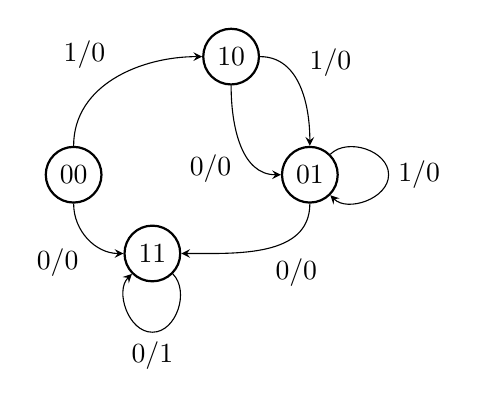
\begin{tikzpicture}
\pgfmathsetmacro{\rad}{0.30}
\draw(0,0)node[]{$00$} node[draw,thick,circle,inner sep=0.25cm](aa){} (2,1.5)node[]{$10$}node[draw,thick,circle,inner sep=0.25cm](ba){} (3,0)node[]{$01$}node[draw,thick,circle,inner sep=0.25cm](ab){} (1,-1)node[]{$11$} node[draw,thick,circle,inner sep=0.25cm](bb){};
\draw[-stealth](aa) to [out=90,in=180]node[pos=0.5,above left]{$1/0$}(ba);
\draw[-stealth](aa) to [out=-90,in=180]node[pos=0.5,below left]{$0/0$}(bb);
\draw[-stealth](ba) to [out=-90,in=180]node[pos=0.5,below left]{$0/0$}(ab);
\draw[-stealth](ba) to [out=0,in=90]node[pos=0.5,above right]{$1/0$}(ab);
\draw[-stealth](ab) to [out=45,in=90] ++(1,0)node[right]{$1/0$} to [out=-90,in=-45] (ab);
\draw[-stealth](bb) to [out=-45,in=0] ++(0,-1)node[below]{$0/1$} to [out=180,in=-135](bb);
\draw[-stealth](ab) to [out=-90,in=0]node[pos=0.5,below right]{$0/0$}(bb);
\end{tikzpicture}
\caption{حال کا خاکہ (برائے شکل \حوالہ{شکل_ترتیبی_بطور_مثال})}
\label{شکل_ترتیبی_خاکہ_حال}
\end{figure}
	


\جزوحصہ{ڈی پلٹ کار پر مبنی ترتیبی دور}
ترتیبی ادوار کے حل کی مزید مثالوں پر غور کرتے ہیں۔پہلی مثال ڈی پلٹ کار پر مبنی ہے جو شکل \حوالہ{شکل_ترتیبی_ڈی_پلٹ_دور} میں پیش ہے۔ دور میں ایک پلٹ کار پایا جاتا ہے جس کا مخارج \عددی{A}لکھ کر، مداخل \عددی{A(x+y)} ہو گا۔

\begin{figure}
\centering
\begin{tikzpicture}
\pgfmathsetmacro{\kshPa}{0.5}
\pgfmathsetmacro{\kshPb}{0.5}
\kDFF[u1]{0}{0}
\draw(u1p1) --++(-3*\kshPa,0)node[above right]{$(x+y)A$}node[and port, scale=1,number inputs=2,anchor=out](u2){} (u2.in 2)--++(-2*\kshPa,0)node[above,xshift=2ex]{$x+y$}node[or port,scale=1,number inputs=2,anchor=out](u3){};
\draw(u3.in 1)node[left]{$x$} (u3.in 2)node[left]{$y$} (u1p2)--++(0,-\kshPa)node[below]{$C$};
\draw(u2.in 1)--++(0,\kshPb)-|(u1p6) --++(\kshPa,0)node[right]{$A$};
\end{tikzpicture}
\caption{ڈی پلٹ کار پر مبنی ترتیبی دور۔}
\label{شکل_ترتیبی_ڈی_پلٹ_دور}
\end{figure}

 ساعت کے کنارہ چڑھائی پر ڈی پلٹ کار مداخل کے تحت نیا حال اختیار کرتا ہے، لہٰذا اگلے حال کی مساوات درج ذیل ہو گی
\begin{align*}
A(n+1)=A(n)(x(n)+y(n))
\end{align*}
جس کی سادہ صورت ذیل ہے۔
\begin{align*}
A=A(x+y)
\end{align*}
اس مساوات کے نتائج شکل \حوالہ{شکل_ڈی_خاکہ_اور_جدول} میں جدول میں پیش ہیں۔حال کا خاکہ اور اس کا سادہ روپ (نچلا خاکہ) بھی شکل پیش ہیں۔ پلٹ کار کے حال \عددی{0} اور \عددی{1} دائروں میں رکھے گئے ہیں، جبکہ ان کے بیچ انتقال تیر دار لکیر سے دکھایا گیا ہے۔ تیر دار لکیروں پر مداخل \عددی{xy} کی موجودہ قیمتیں لکھی گئی ہیں۔ ایک ہی حال میں رہنے کے تمام ممکنات کو اکٹھا بھی لکھا جا سکتا ہے، جیسے نچلے خاکہ میں کیا گیا ہے۔ آپ دیکھ سکتے ہیں کہ حال \عددی{1} سے \عددی{0} اس وقت انتقال ہو گا جب مداخل \عددی{00} ہو۔ باقی تمام حال میں پلٹ کار موجودہ حال برقرار رکھتا ہے۔مزید، حال \عددی{0} سے حال \عددی{1} منتقلی کا کوئی راستہ موجود نہیں۔

\begin{figure}
\centering
\begin{subfigure}{0.35\textwidth}
\centering
\begin{otherlanguage}{english}
\begin{tabular}{CCC|C}
\toprule
\multicolumn{3}{c|}{\text{\RL{موجودہ }}}&{\text{\RL{اگلا }}}\\
\midrule
A&x&y&A\\
\midrule
0&0&0&0\\
0&0&1&0\\
0&1&0&0\\
0&1&1&0\\
1&0&0&0\\
1&0&1&1\\
1&1&0&1\\
1&1&1&1\\
\bottomrule
\end{tabular}
\end{otherlanguage}
\end{subfigure}\hfill
\begin{subfigure}{0.55\textwidth}
\centering
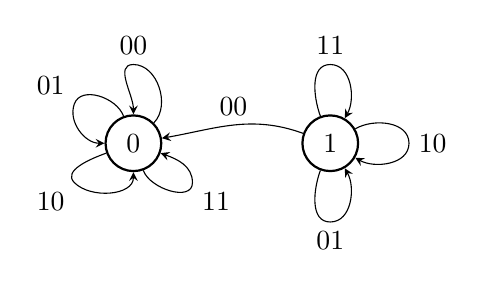
\begin{tikzpicture}
\draw(0,0)node[]{$0$}node[draw,thick,circle,inner sep=0.25cm](a){} (2.5,0)node[]{$1$}node[draw,thick,circle,inner sep=0.25cm](b){};
\draw[-stealth] (b) to [out=160,in=10]node[pos=0.5,above]{$00$}(a);
\draw[-stealth] (b) to [out=110,in=180]++(0,1)node[above]{$11$} to [out=0,in=60] (b);
\draw[-stealth] (b) to [out=30,in=90]++(1,0)node[right]{$10$} to [out=-90,in=-30] (b);
\draw[-stealth] (b) to [out=-110,in=180]++(0,-1)node[below]{$01$} to [out=0,in=-60] (b);
\draw[-stealth] (a) to [out=45,in=0]++(0,1)node[above]{$00$} to [out=180,in=90] (a);
\draw[-stealth] (a) to [out=110,in=70]++(-0.75,0.5)node[above left]{$01$} to [out=-110,in=180] (a);
\draw[-stealth] (a) to [out=-160,in=135]++(-0.75,-0.5)node[below left]{$10$} to [out=-45,in=-90] (a);
\draw[-stealth] (a) to [out=-70,in=-90]++(0.75,-0.5)node[below right]{$11$} to [out=90,in=-20] (a);
\end{tikzpicture}
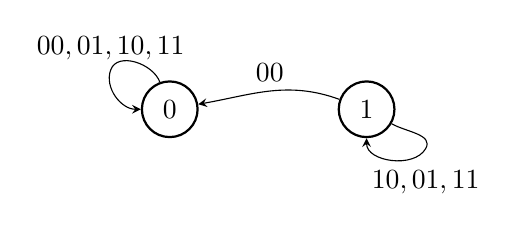
\begin{tikzpicture}
\draw(0,0)node[]{$0$}node[draw,thick,circle,inner sep=0.25cm](a){} (2.5,0)node[]{$1$}node[draw,thick,circle,inner sep=0.25cm](b){};
\draw[-stealth] (b) to [out=160,in=10]node[pos=0.5,above]{$00$}(a);
\draw[-stealth] (b) to [out=-30,in=60]++(0.75,-0.5)node[below,yshift=-1ex]{$10,01,11$} to [out=-120,in=-90] (b);
\draw[-stealth] (a) to [out=110,in=70]++(-0.75,0.5)node[above]{$00,01,10,11$} to [out=-110,in=180] (a);
\end{tikzpicture}
\end{subfigure}
\caption{ حال کا جدول اور حال کا خاکہ (برائے شکل \حوالہ{شکل_ترتیبی_ڈی_پلٹ_دور})}
\label{شکل_ڈی_خاکہ_اور_جدول}
\end{figure}


\جزوحصہ{جے کے پلٹ کار پر مبنی ترتیبی دور}
شکل \حوالہ{شکل_ترتیبی_جے_کے_مثال} میں جے کے پلٹ کار پر مبنی ترتیبی دور پیش ہے۔بالا پلٹ کار کا حال \عددی{Q_A} اور مداخل \عددی{J_A}، \عددی{K_A} ہیں، جبکہ زیریں پلٹ کار کا حال \عددی{Q_B} اور مداخل \عددی{J_B}، \عددی{K_B} ہیں۔

\begin{figure}
\centering
\begin{tikzpicture}
\pgfmathsetmacro{\kshPa}{0.5}
\pgfmathsetmacro{\kshPb}{0.75}
\pgfmathsetmacro{\kshPc}{2.0}
\kJKFF[u1]{0}{0}
\kJKFF[u2]{0}{-\kshPc}
\draw(u1p1)--++(0,\kshPb)--++(-\kshPc,0)node[above right]{$Q_B\overline{x}$}node[and port,scale=1,number inputs=2,anchor=out](u3){};
\draw(u1p3)--++(-\kshPc,0)node[above right]{$Q_B x$}node[and port,scale=1,number inputs=2,anchor=out](u4){};
\draw(u2p3)--++(-\kshPc,0)node[above right]{$\overline{Q_A \oplus x}$}node[xnor port,scale=1,number inputs=2,anchor=out](u5){};
\draw(u3.in 1)--++(-\kshPa,0)node[not port,scale=1,anchor=out](u6){} (u6.in)--++(-\kshPa,0)node[left]{$x$};
\draw(u5.in 2)--++(-\kshPa,0)node[left]{$Q_A$};
\draw(u3.in 2)--(u4.in 1);
\draw(u4.in 1)--++(-\kshPa,0)node[left]{$Q_B$};
\draw(u6.in)|-(u5.in 1);
\draw(u4.in 2)coordinate(aabb)--(aabb -| u6.in);
\draw(u2p1)--(u2p1 -|u6.in);
\draw(u1p2)node[left]{$C$}(u2p2)node[left]{$C$};
\draw(u1p6)node[right]{$Q_A$} (u2p6)node[right]{$Q_B$};
\end{tikzpicture}
\caption{جے کے پلٹ کار پر مبنی ترتیبی دور}
\label{شکل_ترتیبی_جے_کے_مثال}
\end{figure}

 دور میں متمم بلا شرکت جمع گیٹ کا ایک مداخل \عددی{Q_A} ہے جو بالائی پلٹ کار کا موجودہ حال ہے۔ پلٹ کار کے مخارج سے گیٹ کے مداخل تک تار کھینچنے کی بجائے دونوں کا نام \عددی{(Q_A)} رکھا گیا ہے۔ جب بھی دو مقامات کا ایک نام رکھا جائے، انہیں آپس میں برقی طور جڑا تصور کریں۔ یوں ، دونوں ضرب گیٹ کا ایک ایک مداخل زیریں پلٹ کار کے مخارج سے جڑا ہے۔

مداخل کی مساوات ذیل ہیں۔
\begin{gather}
\begin{aligned}\label{مساوات_ترتیبی_جے_کے_بطور_مثال}
J_A&=\overline{x}Q_B\\
K_A&=xQ_B\\
J_B&=x\\
K_B&=\overline{x\oplus Q_A}
\end{aligned}
\end{gather}
ان مساوات سے جدول \حوالہ{جدول_ترتیبی_جے_کے_بطور_مثال} حاصل ہو گا، جس سے اضافی مواد نکال کر حال کا جدول حاصل ہو گا (شکل \حوالہ{شکل_ترتیبی_حال_جے_کے}) ۔  حال  کے جدول سے حاصل حال کا خاکہ بھی شکل میں پیش ہے۔

مساوات \حوالہ{مساوات_ترتیبی_جے_کے_بطور_مثال} سے جدول \حوالہ{جدول_ترتیبی_جے_کے_بطور_مثال} لکھتے ہوئے موجودہ حال \عددی{Q_A}، \عددی{Q_B} اور مداخل \عددی{x} کی تمام ممکنات \عددی{000_2} تا \عددی{111_2} لکھیں (جدول میں بائیں ہاتھ تین قطاریں)۔ ہر صف کے لئے پلٹ کار کے مطابقتی موجودہ مداخل \عددی{J_A}، \عددی{K_A}، \عددی{J_B}،اور \عددی{K_B} مساوات \حوالہ{مساوات_ترتیبی_جے_کے_بطور_مثال} سے حاصل کریں۔ یوں پہلی صف کے لئے، جہاں موجودہ قیمتیں \عددی{Q_A=0}، \عددی{Q_B=0}، اور \عددی{x=0} ہیں، درج ذیل حاصل ہو گا۔
\begin{align*}
J_A&=\overline{x}Q_B=\overline{0}\cdot 0=1\cdot 0=0\\
K_A&=xQ_B=0\cdot 0=0\\
J_B&=x=0\\
K_B&=\overline{x\oplus Q_A}=\overline{0\oplus 0}=\overline{0}=1
\end{align*}
انہیں جدول کی پہلی صف میں درج کریں۔پلٹ کار کے موجودہ مداخل جانتے ہوئے ساعت کے اگلے کنارہ چڑھائی پر اگلے حال مساوات \حوالہ{مساوات_ترتیبی_جے_کے_کارکردگی} \عددی{(Q(n+1)=J\overline{Q}_n+\overline{K}Q_n)} یا مساوات \حوالہ{مساوات_ترتیبی_جے_کے_عام_فہم_کارکردگی} سے 
\begin{align*}
Q_A&=J_A\overline{Q}_A+\overline{K}_AQ_A=0\cdot \overline{0}+\overline{0}\cdot 0=0\cdot 1+1\cdot 0=0+0=0\\
Q_B&=J_B\overline{Q}_B+\overline{K}_BQ_B=0\cdot \overline{0}+\overline{1}\cdot 0= 
\end{align*}
 حاصل کر کے جدول کی پہلی صف میں درج کریں۔ باقی صف کے لئے مواد حاصل کے کے جدول بھریں۔
 
\begin{table}
\caption{جے کے پلٹ کار دور کی مساوات \حوالہ{مساوات_ترتیبی_جے_کے_بطور_مثال} سے حاصل جدول}
\label{جدول_ترتیبی_جے_کے_بطور_مثال}
\centering
\begin{otherlanguage}{english}
\begin{tabular}{CCC|CCCC|CC}
\toprule
\multicolumn{3}{c|}{\text{\RL{موجودہ مداخل اور حال}}} &\multicolumn{4}{c|}{\text{\RL{پلٹ کار کے مداخل}}}&\multicolumn{2}{c}{\text{\RL{اگلے حال}}}\\
\midrule
Q_A&Q_B&x&J_A&K_A&J_B&K_B&Q_A&Q_B\\
\midrule
0&0&0&0&0&0&1&0&0\\
0&0&1&0&0&1&0&0&1\\
\midrule
0&1&0&1&0&0&1&1&0\\
0&1&1&0&1&1&0&0&1\\
\midrule
1&0&0&0&0&0&0&1&0\\
1&0&1&0&0&1&1&1&1\\
\midrule
1&1&0&1&0&0&0&1&1\\
1&1&1&0&1&1&1&0&0\\
\bottomrule
\end{tabular}
\end{otherlanguage}
\end{table}

\begin{figure}
\centering
\begin{subfigure}{0.45\textwidth}
\centering
\begin{otherlanguage}{english}
\begin{tabular}{CCC}
\toprule
\text{\RL{موجودہ حال}} & \multicolumn{2}{c}{\text{\RL{اگلا حال}}}\\
\cline{2-3}
& x=0&x=1\\
Q_AQ_B&Q_AQ_B&Q_AQ_B\\
\midrule
00&00&01\\
01&10&01\\
10&10&11\\
11&11&00\\
\bottomrule
\end{tabular}
\end{otherlanguage}
\end{subfigure}\hfill
\begin{subfigure}{0.45\textwidth}
\centering
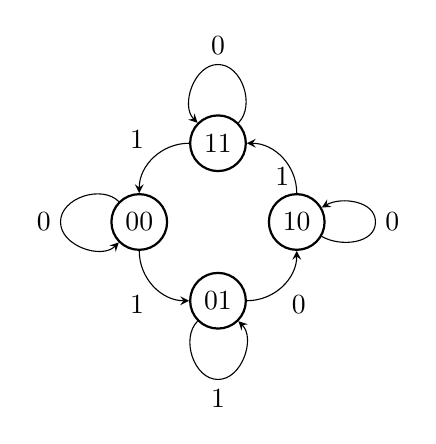
\begin{tikzpicture}
\draw(0,0)node[]{$00$}node[draw,thick,circle,inner sep=0.25cm,](aa){} 
(1,1)node[]{$11$}node[draw,thick,circle,inner sep=0.25cm,](bb){}
(2,0)node[]{$10$}node[draw,thick,circle,inner sep=0.25cm,](ba){}
(1,-1)node[]{$01$}node[draw,thick,circle,inner sep=0.25cm,](ab){};
\draw[-stealth](aa) to [out=-90,in=180]node[pos=0.5,below left]{$1$}(ab);
\draw[-stealth](ab) to [out=0,in=-90]node[pos=0.5,below right]{$0$}(ba);
\draw[-stealth](ba) to [out=90,in=0]node[pos=0.5,below]{$1$}(bb);
\draw[-stealth](bb) to [out=180,in=90]node[pos=0.5,above left]{$1$}(aa);
\draw[-stealth](aa) to [out=135,in=90]++(-1,0)node[left]{$0$} to [out=-90,in=-135](aa);
\draw[-stealth](ab) to [out=-135,in=180]++(0,-1)node[below]{$1$} to [out=0,in=-45](ab);
\draw[-stealth](ba) to [out=-30,in=-90]++(1,0)node[right]{$0$} to [out=90,in=30](ba);
\draw[-stealth](bb) to [out=45,in=0]++(0,1)node[above]{$0$} to [out=180,in=135](bb);
\end{tikzpicture}
\end{subfigure}
\caption{حال کا جدول اور حال کا خاکہ برائے شکل \حوالہ{شکل_ترتیبی_جے_کے_مثال}}
\label{شکل_ترتیبی_حال_جے_کے}
\end{figure}

 
 آپ \عددی{J} اور \عددی{K} کی مساوات استعمال کر کے بھی \عددی{Q} تلاش کر سکتے ہیں۔
 \begin{align*}
 Q_A(n+1)&=J_A\overline{Q}_A+\overline{K}_AQ_A=(\overline{x}Q_B)\overline{Q}_A+(\overline{xQ_B})Q_A\\
 Q_B(n+1)&=J_B\overline{Q}_B+\overline{K}_BQ_B=x\overline{Q}_B+(\overline{\overline{x\oplus Q_A}})Q_B
 \end{align*}

 حال  کے خاکہ (شکل \حوالہ{شکل_ترتیبی_حال_جے_کے}) پر توجہ دیں۔ حال \عددی{00} سے \عددی{01} اور یہاں سے \عددی{10} اور اس کے بعد \عددی{11} جایا جا سکتا ہے، جس کے بعد دوبارہ \عددی{00} سے پوری کہانی شروع ہو گی۔ یہ \عددی{00} تا \عددی{11} ثنائی گنت کار معلوم ہوتا ہے۔ ماسوائے حال \عددی{11} کے، ہر مرتبہ \عددی{x} تبدیل کرنے سے حال تبدیل ہو گا۔ یوں \عددی{00} میں جب تک \عددی{x=0} رہے، دور اسی حال میں رہتا ہے، البتہ \عددی{x} بلند کرنے سے \عددی{01} حال حاصل ہو گا، جہاں اس وقت تک رہا جائے گا جب تک \عددی{x=1} رہے۔



\جزوحصہ{ٹی پلٹ کار کی مدد سے ترتیبی دور کا جائزہ}
شکل \حوالہ{شکل_ترتیبی_ٹی_پلٹ_ترتیبی_مثال} میں ٹی پلٹ کار پر مبنی ترتیبی دور پیش ہے۔ پلٹ کار کے حال \عددی{A} اور \عددی{B} سے ظاہر کیے گئے ہیں۔یوں پہلے پلٹ کار کا مداخل \عددی{T_A} اور دوسرے کا \عددی{T_B} ہے۔
\begin{figure}
\centering
\begin{tikzpicture}
\pgfmathsetmacro{\kshY}{2.00}
\pgfmathsetmacro{\kshPa}{0.75}
\pgfmathsetmacro{\kshPb}{0.75}
\kTFF[u1]{0}{0}
\kTFF[u2]{0}{-\kshY}
\draw(u1p1)--++(-\kshPa,0)node[and port,scale=1,number inputs=2,anchor=out](u3){};
\draw(u2p1)node[nor port,scale=1,number inputs=2,anchor=out](u4){};
\draw(u3.out)--++(0,-\kshPb)-|(u4.in 1);
\draw(u1p2)--(u2p2)--++(0,-\kshPb)--++(-0.5,0)node[left]{$C$};
\draw(u3.in 1)node[left]{$A$} (u3.in 2)node[left]{$\overline{B}$} (u4.in 2)node[left]{$x$};
\draw(u1p6)node[right]{$A$} (u1p4)node[right]{$\overline{A}$}
(u2p6)node[right]{$B$} (u2p4)node[right]{$\overline{B}$};
\end{tikzpicture}
\caption{ٹی پلٹ کار پر مبنی ترتیبی دور}
\label{شکل_ترتیبی_ٹی_پلٹ_ترتیبی_مثال}
\end{figure}

پلٹ کار کا اگلا حال مساوات \حوالہ{مساوات_ترتیبی_ٹی_پلٹ_کی_مساوات} سے ملتا ہے جسے یہاں دوبارہ پیش کرتے ہیں۔
\begin{align*}
Q_{n+1}=T\oplus Q_n
\end{align*}
موجودہ ضرورت کے تحت مساوات سے درج ذیل لکھا جاتا ہے۔
\begin{gather}
\begin{aligned}\label{مساوات_ترتیبی_ٹی_مثال_حال}
A_{n+1}&=T_A\oplus A=T_A \overline{A}+\overline{T}_AA\\
B_{n+1}&=T_B\oplus B=T_B\overline{B}+\overline{T}_BB
\end{aligned}
\end{gather}

پلٹ کار کے مداخل کی مساوات شکل \حوالہ{شکل_ترتیبی_ٹی_پلٹ_ترتیبی_مثال} سے حاصل کرتے ہیں۔
\begin{align*}
T_A&=A\overline{B}\\
T_B&=\overline{A\overline{B}+x}
\end{align*}
ان مساوات کو مساوات \حوالہ{مساوات_ترتیبی_ٹی_مثال_حال} میں ڈالنے سے پلٹ کار کے حال کی مساواتیں حاصل ہوں گی:
\begin{align*}
A_{n+1}&=(A\overline{B})\oplus A\\
B_{n+1}&=(\overline{A\overline{B}+x})\oplus B
\end{align*}
جن سے جدول \حوالہ{جدول_ترتیبی_ٹی_پلٹ_بطور_مثال}-الف ملتا ہے۔ مداخل \عددی{x} اور موجودہ حال \عددی{A} اور \عددی{B} کو پہلی تین قطاروں میں لکھا گیا ہے۔ ان کی تمام ترتیب (\عددی{000_2} تا \عددی{111_2}) پہلی تین قطاروں میں بھر کر، ہر صف کے لئے مطابقتی موجودہ مداخل حاصل کیے جاتے ہیں، جنہیں دائیں قطاروں میں لکھا گیا ہے۔ موجودہ مداخل سے ساعت کے اگلے کنارہ چڑھائی پر اگلے حال حاصل ہوں گے۔ جدول \حوالہ{جدول_ترتیبی_ٹی_پلٹ_بطور_مثال}-الف سے جدول-ب لکھا جا سکتا ہے، جو حال کا جدول کہلاتا ہے۔
\begin{table}
\caption{ٹی پلٹ کار دور (شکل \حوالہ{شکل_ترتیبی_ٹی_پلٹ_ترتیبی_مثال}) کا حال کا جدول}
\label{جدول_ترتیبی_ٹی_پلٹ_بطور_مثال}
\centering
\begin{subtable}{0.6\textwidth}
\caption{}
\centering
\begin{otherlanguage}{english}
\begin{tabular}{CCC|CC|CC}
\toprule
\multicolumn{3}{c}{\text{\RL{موجودہ مواد}}}&\multicolumn{2}{|c|}{\text{\RL{اگلا حال}}} &\multicolumn{2}{c}{\text{\RL{مداخل}}}\\
\midrule
A&B&x&A&B&T_A&T_B\\
\midrule
0&0&0&0&1&0&1\\
0&0&1&0&0&0&0\\
\midrule
0&1&0&0&0&0&1\\
0&1&1&0&1&0&0\\
\midrule
1&0&0&0&0&1&0\\
1&0&1&0&0&1&0\\
\midrule
1&1&0&1&0&0&1\\
1&1&1&1&1&0&0\\
\bottomrule
\end{tabular}
\end{otherlanguage}
\end{subtable}\hfill
\begin{subtable}{0.4\textwidth}
\caption{}
\centering
\begin{otherlanguage}{english}
\begin{tabular}{CCC}
\toprule
\text{\RL{موجودہ}}&\multicolumn{2}{c}{\text{\RL{اگلا حال}}}\\
\cline{2-3}
&x=0&x=1\\
AB&AB&AB\\
\midrule
00&01&00\\
01&00&01\\
10&00&00\\
11&10&11\\
\bottomrule
\end{tabular}
\end{otherlanguage}
\end{subtable}
\end{table}

 حال  کے جدول کے مواد کو  حال  کے خاکہ کی صورت میں شکل \حوالہ{شکل_ترتیبی_ڈی_پلٹ_بطور_مثال_خاکہ_حال} میں پیش کیا گیا ہے۔ جدول \حوالہ{جدول_ترتیبی_ٹی_پلٹ_بطور_مثال}-ب میں \عددی{AB} کو ساتھ ساتھ لکھ کر ایک حال تصور کریں۔یوں \عددی{00}، \عددی{01}،\عددی{10}،اور \عددی{11} حال ممکن ہیں۔  حال  کے خاکہ میں حال کو گول دائرہ میں لکھا جاتا ہے، اور ایک حال سے دوسرے حال (یا اسی حال) انتقال کو تیر دار لکیر سے ظاہر کیا جاتا ہے،جن پر آزاد مداخل \عددی{(x)} کی وہ قیمت درج کی جاتی ہے، جو انتقال کا سبب بنتی ہے۔ مثلاً، جدول-ب کی پہلی صف میں موجودہ حال \عددی{00} ہے؛ اب \عددی{x=1} کی صورت میں دور اسی حال \عددی{(00)} میں رہتا ہے، جس کو حال  کے خاکہ میں \عددی{00}حال سے ابتدا اور اختتام کرنے والی تیر دار لکیر سے ظاہر کیا گیا ہے، جس پر \عددی{1} لکھا گیا ہے؛ البتہ \عددی{x=0} کی صورت میں دور حال \عددی{01} اختیار کرتا ہے،جس کو \عددی{00} سے \عددی{01} جانے والی تیر دار لکیر ظاہر کرتی ہے، جس پر \عددی{0} لکھا گیا ہے ۔

\begin{figure}
\centering
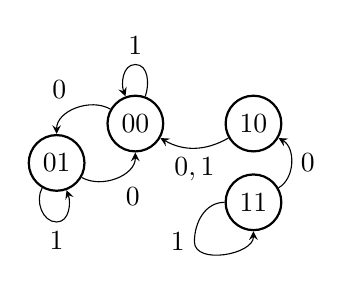
\begin{tikzpicture}
\draw(0,0.5)node[]{$00$}node[draw,thick,circle,inner sep=0.25cm](aa){};
\draw(-1,0)node[]{$01$}node[draw,thick,circle,inner sep=0.25cm](ab){};
\draw(1.5,0.5)node[]{$10$}node[draw,thick,circle,inner sep=0.25cm](ba){};
\draw(1.5,-0.5)node[]{$11$}node[draw,thick,circle,inner sep=0.25cm](bb){};
\draw[-stealth](aa) to [out=70,in=0]++(0,0.75)node[above]{$1$} to [out=180,in=110] (aa);
\draw[-stealth](ab) to [out=-120,in=-180]++(0,-0.75)node[below]{$1$} to [out=0,in=-70] (ab);
\draw[-stealth](bb) to [out=180,in=90]++(-0.75,-0.5)node[left]{$1$} to [out=-90,in=-90] (bb);
\draw[-stealth](aa) to [out=150,in=90] node[pos=0.5,above left]{$0$}(ab);
\draw[-stealth](ab) to [out=-30,in=-90] node[pos=0.5,below right]{$0$}(aa);
\draw[-stealth](ba) to [out=-150,in=-30] node[pos=0.5,below]{$0,1$}(aa);
\draw[-stealth](bb) to [out=30,in=-30] node[pos=0.5,right]{$0$}(ba);
\end{tikzpicture}
\caption{حال کا خاکہ برائے شکل \حوالہ{شکل_ترتیبی_ٹی_پلٹ_ترتیبی_مثال} اور جدول \حوالہ{جدول_ترتیبی_ٹی_پلٹ_بطور_مثال}}
\label{شکل_ترتیبی_ڈی_پلٹ_بطور_مثال_خاکہ_حال}
\end{figure}


\حصہ{میلی اور مُور نمونہ}
 ترتیبی دور میں مداخل، مخارج اور اندرونی حال پائے جاتے ہیں۔ترتیبی ادوار کے دو نمونے پائے جاتے ہیں، جنہیں \اصطلاح{میلی نمونہ}\فرہنگ{میلی نمونہ}\حاشیہب{Mealy}\فرہنگ{Mealy} اور \اصطلاح{مُور نمونہ}\فرہنگ{مور نمونہ}\حاشیہب{Moore}\فرہنگ{Moore} کہتے ہیں۔میلی نمونہ میں مخارج کا دارومدار موجودہ مداخل اور موجودہ اندونی حال پر ، جبکہ مُور نمونہ میں صرف موجودہ حال پر ہو گا۔یہ دو نمونے شکل \حوالہ{شکل_ترتیبی_مور_میلی} میں پیش ہیں۔
 
 ان اشکال میں مداخل تیر دار لکیر پر ترچھی لکیر کھینچ کر \عددی{X} لکھا گیا ہے، جو مداخل ثنائی ہندسوں (بِٹ) کی تعداد بیان کرتا ہے۔ یوں \عددی{X=8} کی صورت میں ایک ایک بٹ کے آٹھ مداخل ہوں گے۔ حافظہ کے مداخل اور مخارج کی تعداد برابر ہو گی، لہٰذا اس کے مداخل (یا مخارج) پر \عددی{Y} لکھنے کے بعد مخارج (یا مداخل) پر صرف ترچھی لکیر کھینچنا کافی ہو گا۔
\begin{figure}
\centering
\begin{subfigure}{0.45\textwidth}
\centering
\begin{tikzpicture}
\pgfmathsetmacro{\kdimX}{1.5}
\pgfmathsetmacro{\kdimY}{0.75}
\pgfmathsetmacro{\ksepY}{1.00}
\pgfmathsetmacro{\kshPa}{1.0}
\pgfmathsetmacro{\kshPb}{0.5}
\pgfmathsetmacro{\kdel}{0.1}
\draw[thick](0,0) rectangle ++(\kdimX,\kdimY)node[pos=0.5]{\text{\RL{ترکیبی منطق}}};
\draw[thick](0,-\ksepY) rectangle ++(\kdimX,\kdimY)node[pos=0.5]{\text{\RL{حافظہ}}};
\draw[stealth-] (0,0.75*\kdimY)--++(-\kshPa,0)coordinate[pos=0.5](aa)node[left]{مداخل};
\draw(aa)++(-\kdel,-\kdel)--++(2*\kdel,2*\kdel)node[above]{$X$};
\draw[-stealth] (\kdimX,0.75*\kdimY)--++(\kshPa,0)coordinate[pos=0.5](bb)node[right]{مخارج};
\draw(bb)++(-\kdel,-\kdel)--++(2*\kdel,2*\kdel)node[above]{$Z$};
\draw[-stealth](\kdimX,0.25*\kdimY)--++(\kshPb,0)|-(\kdimX,-\ksepY+0.5*\kdimY);
\draw[-stealth](0,-\ksepY+0.5*\kdimY)--++(-\kshPb,0)|-(0,0.25*\kdimY);
\draw(-\kshPb,-\ksepY/2+\kdimY/2-0.125*\kdimY)++(\kdel,-\kdel)--++(-2*\kdel,2*\kdel)node[left]{$Y$};
\draw(\kdimX+\kshPb,-\ksepY/2+\kdimY/2-0.125*\kdimY)++(-\kdel,-\kdel)--++(2*\kdel,2*\kdel)node[right]{$Y$};
\end{tikzpicture}
\caption{میلی نمونہ}
\end{subfigure}\hfill
\begin{subfigure}{0.45\textwidth}
\centering
\begin{tikzpicture}
\pgfmathsetmacro{\kdimX}{1.5}
\pgfmathsetmacro{\kdimY}{0.75}
\pgfmathsetmacro{\ksepY}{1.00}
\pgfmathsetmacro{\kshPa}{1.0}
\pgfmathsetmacro{\kshPb}{0.5}
\pgfmathsetmacro{\kdel}{0.1}
\draw[thick](0,0) rectangle ++(\kdimX,\kdimY)node[pos=0.5]{\text{\RL{ترکیبی منطق}}};
\draw[thick](0,-\ksepY) rectangle ++(\kdimX,\kdimY)node[pos=0.5]{\text{\RL{حافظہ}}};
\draw[thick](0,-2*\ksepY) rectangle ++(\kdimX,\kdimY)node[pos=0.5]{\text{\RL{ترکیبی منطق}}};
\draw[stealth-] (0,0.75*\kdimY)--++(-\kshPa,0)coordinate[pos=0.5](aa)node[left]{مداخل};
\draw(aa)++(-\kdel,-\kdel)--++(2*\kdel,2*\kdel)node[above]{$X$};
\draw[-stealth] (\kdimX,-2*\ksepY+0.75*\kdimY)--++(\kshPa,0)coordinate[pos=0.5](bb)node[right]{مخارج};
\draw(bb)++(-\kdel,-\kdel)--++(2*\kdel,2*\kdel)node[above]{$Z$};
\draw[-stealth](\kdimX,0.25*\kdimY)--++(\kshPb,0)|-(\kdimX,-\ksepY+0.5*\kdimY);
\draw[-stealth](0,-\ksepY+0.5*\kdimY)--++(-\kshPb,0)coordinate(dd)|-(0,0.25*\kdimY);
\draw(-\kshPb/2,-\ksepY+\kdimY/2)++(\kdel,-\kdel)--++(-2*\kdel,2*\kdel);
\draw(\kdimX+\kshPb,-\ksepY/2+\kdimY/2-0.125*\kdimY)++(-\kdel,-\kdel)--++(2*\kdel,2*\kdel)node[right]{$Y$};
\draw[-stealth](dd)|-(0,-2*\ksepY+\kdimY/2);
\end{tikzpicture}
\caption{مور نمونہ}
\end{subfigure}
\caption{مور اور میلی نمونے}
\label{شکل_ترتیبی_مور_میلی}
\end{figure}

%???KKK
%this heading makes no sense

\جزوحصہ{حال اور ان کی مقرری}
حصہ \حوالہ{حصہ_ترتیبی_خاکہ_حال} میں  حال  کے خاکہ پر غور کیا گیا۔ ان خاکوں میں پلٹ کار کے مخارج کی بجائے دیگر ناموں سے حال ظاہر کر کے حال  کا خاکہ سمجھنا آسان بنایا جا سکتا ہے (درج ذیل مثال دیکھیں)۔


\ابتدا{مثال}\شناخت{مثال_ترتیبی_حال_کے_نام}
ایسے ایک مداخل، ایک مخارج معاصر ترتیبی دور کا حال کا خاکہ تیار کریں، جو \عددی{110_2} مداخل کے حصول پر \عددی{1} خارج کرتا ہو۔ بلند رتبی بِٹ پہلا بِٹ تصور کریں۔ایسے دور کو \اصطلاح{ترتیب شناس}\فرہنگ{ترتیب!شناس}\حاشیہب{sequence detector}\فرہنگ{sequence!detector} کہتے ہیں۔ 

\begin{figure}
\centering
\begin{tikzpicture}[every text node part/.style={align=center}]
\draw(0,0)node[draw,thick,ellipse,inner sep=0pt](a){\text{\RL{\,\,\, ابتدا \,\,\,}} \\ $0$};
\draw(2,1)node[draw,thick,ellipse,inner sep=0pt](b){\text{\RL{پہلا ایک مل گیا}} \\ $0$};
\draw(6,1)node[draw,thick,ellipse,inner sep=0pt](c){\text{\RL{دوسرا ایک مل گیا}} \\ $0$};
\draw(8,0)node[draw,thick,ellipse,inner sep=0pt](d){\text{\RL{ترتیب مل گئی}} \\ $1$};
\draw[-stealth](a) to [out=90,in=180] node[pos=0.5,above left]{$1$}(b);
\draw[-stealth](b) to [out=30,in=150] node[pos=0.5,above]{$1$}(c);
\draw[-stealth](c) to [out=0,in=60] node[pos=0.5,above right]{$0$}(d);
\draw[-stealth](d) to [out=180,in=-20] node[pos=0.5,above]{$0,1$}(a);
\draw[-stealth](a) to [out=-170,in=-90]++(-1.5,0)node[left]{$0$} to [out=90,in=170] (a);
\draw[-stealth](c) to [out=110,in=180]++(0,1)node[above]{$1$} to [out=0,in=70] (c);
\draw[-stealth](b) to [out=-100,in=10] node[pos=0.5,above left]{$0$}(a);
\end{tikzpicture}
\caption{حال کو الفاظ سے پکار کر خاکہ بہتر سمجھ آتا ہے (مثال \حوالہ{مثال_ترتیبی_حال_کے_نام})}
\label{شکل_ترتیبی_مثال_حال_کے_نام}
\end{figure}
\ترچھا{حل:}\quad
شکل \حوالہ{شکل_ترتیبی_مثال_حال_کے_نام} میں حال کا خاکہ پیش ہے، جسے دیکھ کر دور کی کارکردگی سمجھنا آسان ہے۔ دائرے میں حال کا نام، اور نام کے نیچے \عددی{0} یا \عددی{1} موجودہ مخارج ظاہر کرتا ہے۔
\انتہا{مثال}

\حصہ{معاصر ترتیبی ادوار کی بناوٹ}
گزشتہ حصے میں مختلف اقسام کے پلٹ کار استعمال کر کے معاصر ترتیبی ادوار تشکیل دیے گئے۔ان ادوار کے حصول کا باضابطہ طریقہ کار درج ذیل ہے۔
\begin{enumerate}
 \item
 مسئلہ کے بیان سے حال کا خاکہ تیار کریں۔
 \item
 درکار حال کی تعداد کم کریں۔
 \item
 ہر حال (کو ظاہر کرنے) کی منفرد ثنائی قیمت منتخب کریں۔
 \item
 حال کا جدول حاصل کریں۔
 \item
 پلٹ کار (کی قسم) کا انتخاب کریں۔
 \item
 پلٹ کار کی داخلی اور خارجی سادہ ترین مساوات حاصل کریں۔
 \item
 ان مساوات سے معاصر ترتیبی دور تشکیل دیں۔
\end{enumerate}
 
\ابتدا{مثال}\شناخت{مثال_ترتیبی_تین_ایک_شناس}
 ایسا معاصر ترتیب شناس تشکیل دیں جو تین متواتر \عددی{1}مداخل کے حصول پر \عددی{1}خارج کرے۔ 
\begin{figure}
\centering
\begin{subfigure}{0.60\textwidth}
\centering
\begin{tikzpicture}
\pgfmathsetmacro{\shPa}{1.5}
\draw[](0,0)node[]{$a/0$}node[draw,thick,circle,inner sep=0.25cm](aa){} (aa.west)node[left]{\text{\RL{ابتدا}}};
\draw[](1*\shPa,0)node[]{$b/0$}node[draw,thick,circle,inner sep=0.25cm](ab){};
\draw[](2*\shPa,0)node[]{$c/0$}node[draw,thick,circle,inner sep=0.25cm](ba){};
\draw[](3*\shPa,0)node[]{$d/1$}node[draw,thick,circle,inner sep=0.25cm](bb){};
\draw[-stealth](aa) to [out=70,in=0]++(0,0.75)node[above]{$0$} to [out=180,in=110] (aa);
\draw[-stealth](aa) to [out=45,in=135] node[pos=0.5,above]{$1$}(ab);
\draw[-stealth](ab) to [out=-90,in=-30]node[pos=0.6,above]{$0$} (aa);
\draw[-stealth](ab) to [out=45,in=135] node[pos=0.5,above]{$1$}(ba);
\draw[-stealth](ba) to [out=-135,in=-45]node[pos=0.25,above]{$0$} (aa);
\draw[-stealth](ba) to [out=45,in=135] node[pos=0.5,above]{$1$}(bb);
\draw[-stealth](bb) to [out=70,in=0]++(0,0.75)node[above]{$1$} to [out=180,in=110] (bb);
\draw[-stealth](bb) to [out=-135,in=-60]node[pos=0.25,above]{$0$} (aa);
\end{tikzpicture}
\end{subfigure}\hfill
\begin{subfigure}{0.4\textwidth}
\centering
\begin{otherlanguage}{english}
\begin{tabular}{CC|CC}
\toprule
\multicolumn{2}{c|}{\text{\RL{موجودہ}}}&\text{\RL{اگلا}}&\text{\RL{موجودہ}}\\
\text{\RL{حال}}&\text{\RL{مداخل}}&\text{\RL{حال}}&\text{\RL{مخارج}}\\
\midrule
a&0&a&0\\
a&1&b&0\\
b&0&a&0\\
b&1&c&0\\
c&0&a&0\\
c&1&d&0\\
d&0&a&1\\
d&1&d&1\\
\bottomrule
\end{tabular}
\end{otherlanguage}
\end{subfigure}
\caption{ترتیب شناس کا حال کا خاکہ ( مثال \حوالہ{مثال_ترتیبی_تین_ایک_شناس})}
\label{شکل_ترتیبی_تین_ایک_شناس}
\end{figure}

\ترچھا{حل:}\quad
ترتیب شناس کی کارکردگی کے بیان سے شکل \حوالہ{شکل_ترتیبی_تین_ایک_شناس} کا حال کا خاکہ کھینچا جاتا ہے۔گول دائروں میں ترچھی لکیر سے اوپر حال کا نام اور نیچے مخارج کی قیمت لکھی گئی ہے۔ شناس کا ابتدائی حال \عددی{a} اور مخارج پست \عددی{(0)} ہے۔ پہلی  \عددی{1} کی  حصول کے بعد حال \عددی{b} اور مخارج پست ہو گا۔ دوسری  \عددی{1} کے بعد حال \عددی{c} اور مخارج پست، تیسری \عددی{1} کے بعد حال \عددی{d} اور مخارج بلند ہو گا۔ مزید \عددی{1} ملنے سے شناس حال \عددی{d} میں رہتے ہوئے مخارج بلند رکھتا ہے۔ کسی بھی موقع پر \عددی{0} کا حصول، شناس کو واپس ابتدائی حال \عددی{a} منتقل کرتا ہے۔ حال  کے خاکہ سے حاصل جدول، شکل \حوالہ{شکل_ترتیبی_تین_ایک_شناس} میں پیش ہے، جس میں بائیں ہاتھ موجودہ مداخل اور موجودہ حال، جبکہ دائیں ہاتھ اگلا حال اور موجودہ مخارج درج ہیں۔

حال  کے خاکہ سے واضح ہے کہ حال کی تعداد چار ہے، جنہیں دو بِٹ کا ثنائی عدد ظاہر کر سکتا ہے۔
\begin{gather}
\begin{aligned}\label{مساوات_ترتیبی_شناس_حال_انتخاب}
a&=00\\
b&=01\\
c&=10\\
d&=11
\end{aligned}
\end{gather}
(آپ کوئی دوسری انتخاب کر سکتے ہیں۔ مشق \حوالہ{مشق_ترتیبی_شناس} دیکھیں۔) دو بِٹ کے لئے دو پلٹ کار درکار ہوں گے۔ ہم ڈی پلٹ کار منتخب کر کے، ان کے مخارج \عددی{A} اور \عددی{B}، اور مداخل \عددی{D_A} اور \عددی{D_B} لکھتے ہیں۔

ثنائی علامت استعمال کرتے ہوئے شکل \حوالہ{شکل_ترتیبی_تین_ایک_شناس} میں پیش جدول دوبارہ جدول \حوالہ{جدول_ترتیبی_ترتیب_شناس_متواتر_ایک} میں پیش کیا گیا ہے، جس سے ڈی پلٹ کار کی درج ذیل مساوات اخذ ہوتی ہیں۔
\begin{align*}
A(n+1)=D_A(A,B,x)&=\sum(3,5,7)\\
B(n+1)=D_B(A,B,x)&=\sum(1,5,7)\\
y(A,B,x)&=\sum(6,7)
\end{align*}

\begin{table}
\caption{ترتیب شناس  کا حال کا جدول}
\label{جدول_ترتیبی_ترتیب_شناس_متواتر_ایک}
\centering
\begin{otherlanguage}{english}
\begin{tabular}{CCC|CCC}
\toprule
\multicolumn{3}{c|}{\text{\RL{موجودہ}}}&\multicolumn{2}{c}{\text{\RL{اگلا}}}&\text{\RL{موجودہ}}\\
\cline{4-5}
A&B&x&A&B&y\\
\midrule
0&0&0&0&0&0\\
0&0&1&0&1&0\\
0&1&0&0&0&0\\
0&1&1&1&0&0\\
1&0&0&0&0&0\\
1&0&1&1&1&0\\
1&1&0&0&0&1\\
1&1&1&1&1&1\\
\bottomrule
\end{tabular}
\end{otherlanguage}
\end{table}
%
\begin{figure}
\centering
\begin{subfigure}{0.3\textwidth}
\centering
\begin{tikzpicture}
\pgfmathsetmacro{\kxstep}{1}
\pgfmathsetmacro{\kystep}{1}
\pgfmathsetmacro{\kpin}{0.75}
\pgfmathsetmacro{\kmv}{0.15}
\pgfmathsetmacro{\kmva}{0.10}
\draw[xstep=\kxstep,ystep=\kystep](0,0) grid (2*\kxstep,-4*\kystep);
\draw(0,0)--++(135:\kpin)node[pos=0.75,above right]{$x$}node[pos=0.75,below left]{$AB$};
\foreach \kx/\xlb in {0/0,1/1}{\draw(\kx*\kxstep+\kxstep/2,0)node[above]{$\xlb$};}
\foreach \ky/\ylb in {0/{00},1/{01},2/{11},3/{10}}{\draw(0,-\ky*\kystep-\kystep/2)node[left]{$\ylb$};}
\foreach \ky/\ylb in {0/{0},1/{0},2/{0},3/{0}}{\draw(\kxstep/2,-\ky*\kystep-\kystep/2)node[]{$\ylb$};}
\foreach \ky/\ylb in {0/{0},1/{1},2/{1},3/{1}}{\draw(\kxstep+\kxstep/2,-\ky*\kystep-\kystep/2)node[]{$\ylb$};}
\draw[gray,dashed] ($(\kxstep,-1*\kystep)+(\kmv,-\kmv)$) rectangle ($(2*\kxstep,-3*\kystep)+(-\kmv,\kmv)$);
\draw[gray,dashed] ($(\kxstep,-2*\kystep)+(1.5*\kmv,-1.5*\kmv)$) rectangle ($(2*\kxstep,-4*\kystep)+(-1.5*\kmv,1.5*\kmv)$);
\draw(1*\kxstep,-4*\kystep)node[below]{$D_A=xA+xB$};
\end{tikzpicture}
\end{subfigure}\hfill
\begin{subfigure}{0.3\textwidth}
\centering
\begin{tikzpicture}
\pgfmathsetmacro{\kxstep}{1}
\pgfmathsetmacro{\kystep}{1}
\pgfmathsetmacro{\kpin}{0.75}
\pgfmathsetmacro{\kmv}{0.15}
\pgfmathsetmacro{\kmva}{0.10}
\draw[xstep=\kxstep,ystep=\kystep](0,0) grid (2*\kxstep,-4*\kystep);
\draw(0,0)--++(135:\kpin)node[pos=0.75,above right]{$x$}node[pos=0.75,below left]{$AB$};
\foreach \kx/\xlb in {0/0,1/1}{\draw(\kx*\kxstep+\kxstep/2,0)node[above]{$\xlb$};}
\foreach \ky/\ylb in {0/{00},1/{01},2/{11},3/{10}}{\draw(0,-\ky*\kystep-\kystep/2)node[left]{$\ylb$};}
\foreach \ky/\ylb in {0/{0},1/{0},2/{0},3/{0}}{\draw(\kxstep/2,-\ky*\kystep-\kystep/2)node[]{$\ylb$};}
\foreach \ky/\ylb in {0/{1},1/{0},2/{1},3/{1}}{\draw(\kxstep+\kxstep/2,-\ky*\kystep-\kystep/2)node[]{$\ylb$};}
\draw[gray,dashed] ($(\kxstep,-0*\kystep)+(\kmv,\kmv)$) --++ ($(0*\kxstep,-1*\kystep)+(-0*\kmv,0*\kmv)$)--++($(1*\kxstep,0)+(-2*\kmv,0)$)--++($(0,\kystep)+(0,0*\kmv)$);
\draw[gray,dashed] ($(\kxstep,-4*\kystep)+(\kmv,-\kmv)$) --++ ($(0*\kxstep,1*\kystep)+(-0*\kmv,0*\kmv)$)--++($(1*\kxstep,0)+(-2*\kmv,0)$)--++($(0,-\kystep)+(0,0*\kmv)$);
\draw[gray,dashed] ($(\kxstep,-2*\kystep)+(1.5*\kmv,-1.5*\kmv)$) rectangle ($(2*\kxstep,-4*\kystep)+(-1.5*\kmv,1.5*\kmv)$);
\draw(1*\kxstep,-4*\kystep)node[below]{$D_B=xA+x\overline{B}$};
\end{tikzpicture}
\end{subfigure}\hfill
\begin{subfigure}{0.3\textwidth}
\centering
\begin{tikzpicture}
\pgfmathsetmacro{\kxstep}{1}
\pgfmathsetmacro{\kystep}{1}
\pgfmathsetmacro{\kpin}{0.75}
\pgfmathsetmacro{\kmv}{0.15}
\pgfmathsetmacro{\kmva}{0.10}
\draw[xstep=\kxstep,ystep=\kystep](0,0) grid (2*\kxstep,-4*\kystep);
\draw(0,0)--++(135:\kpin)node[pos=0.75,above right]{$x$}node[pos=0.75,below left]{$AB$};
\foreach \kx/\xlb in {0/0,1/1}{\draw(\kx*\kxstep+\kxstep/2,0)node[above]{$\xlb$};}
\foreach \ky/\ylb in {0/{00},1/{01},2/{11},3/{10}}{\draw(0,-\ky*\kystep-\kystep/2)node[left]{$\ylb$};}
\foreach \ky/\ylb in {0/{0},1/{0},2/{1},3/{0}}{\draw(\kxstep/2,-\ky*\kystep-\kystep/2)node[]{$\ylb$};}
\foreach \ky/\ylb in {0/{0},1/{0},2/{1},3/{0}}{\draw(\kxstep+\kxstep/2,-\ky*\kystep-\kystep/2)node[]{$\ylb$};}
\draw[gray,dashed] ($(0*\kxstep,-2*\kystep)+(\kmv,-\kmv)$) rectangle ($(2*\kxstep,-3*\kystep)+(-\kmv,\kmv)$);
\draw(1*\kxstep,-4*\kystep)node[below]{$y=AB$};
\end{tikzpicture}
\end{subfigure}
\caption{کارناف نقشے برائے مثال \حوالہ{مثال_ترتیبی_تین_ایک_شناس} }
\label{شکل_ترتیبی_مثال_کارناف}
\end{figure}

جدول \حوالہ{جدول_ترتیبی_ترتیب_شناس_متواتر_ایک} سے شکل \حوالہ{شکل_ترتیبی_مثال_کارناف} کے کارناف نقشے بنا کر درج ذیل سادہ مساوات حاصل ہوتی ہیں،جن سے 
شکل \حوالہ{شکل_ترتیبی_شناس_مثال} حاصل ہو گا۔
\begin{align*}
D_A&=Ax+Bx\\
D_B&=Ax+\overline{B}x\\
y&=AB
\end{align*}
%
\begin{figure}
\centering
\begin{tikzpicture}
\pgfmathsetmacro{\kshPa}{0.75}
\pgfmathsetmacro{\kshPb}{0.35}
\pgfmathsetmacro{\kshPc}{0.5}
\pgfmathsetmacro{\kshYa}{2.5}
\kDFF[u1]{0}{0}
\kDFF[u2]{0}{-\kshYa}
\draw($(u1p6)!0.5!(u2p6)$)++(3*\kshPa,0)node[and port, scale=1,number inputs=2,anchor=out](u3){};
\draw(u1p6)-|(u3.in 1) (u2p6)-|(u3.in 2) (u3.out)node[right]{$y$};
\draw(u1p1)--++(-\kshPa,0)node[or port,scale=1,number inputs=2,anchor=out](u4){};
\draw(u4.in 1)--++(0,\kshPb)node[and port,scale=1,number inputs=2,anchor=out](u5){};
\draw(u4.in 2)--++(0,-\kshPb)node[and port,scale=1,number inputs=2,anchor=out](u6){};
\draw(u2p1)--++(-\kshPa,0)node[or port,scale=1,number inputs=2,anchor=out](u7){};
\draw(u7.in 1)--++(0,\kshPb)node[and port,scale=1,number inputs=2,anchor=out](u8){};
\draw(u7.in 2)--++(0,-\kshPb)node[and port,scale=1,number inputs=2,anchor=out](u9){};
\draw(u1p6)node[above]{$A$} (u2p6)node[above]{$B$};
\draw(u5.in 1)--++(-\kshPc,0)node[left]{$A$} (u5.in 2)--(u6.in 1) (u5.in 2)--++(-\kshPc,0)node[left]{$x$}
 (u6.in 2)--++(-\kshPc,0) node[left]{$B$};
\draw(u8.in 1)--++(-\kshPc/2,0)coordinate(kaa)--(kaa |- u5.in 1) (u8.in 2)--(u9.in 1) (u8.in 2)--(u6.in 1)
 (u9.in 2)--++(-\kshPc,0)node[left]{$\overline{B}$};
 \draw(u1p2)--(u2p2)--++(0,-\kshPc)--++(-\kshPc,0)node[left]{$C$};
 \draw(u4.out)node[above]{$D_A$} (u7.out)node[above]{$D_B$};
 \draw(u2p4)node[above]{$\overline{B}$};
\end{tikzpicture}
\caption{ترتیب شناس (مثال \حوالہ{مثال_ترتیبی_تین_ایک_شناس})}
\label{شکل_ترتیبی_شناس_مثال}
\end{figure}
ترتیب شناس ابتدائی پست حال میں \عددی{\overline{\text{بیٹھ}}} اشارہ کی مدد سے لایا جاتا ہے، جو شکل میں نہیں دکھایا گیا۔
\انتہا{مثال}
%
\ابتدا{مشق}\شناخت{مشق_ترتیبی_شناس}
مساوات \حوالہ{مساوات_ترتیبی_شناس_حال_انتخاب} میں حال کے اظہار کا ایک انتخاب دکھایا گیا ہے۔آپ کوئی دوسرا انتخاب کر سکتے ہیں، مثلاً \عددی{a=01}، \عددی{b=10}، \عددی{c=11}، اور \عددی{d=00} جس سے دوسرا دور حاصل ہو گا۔ یہ دور حاصل کریں۔
\انتہا{مشق}

\حصہء{سوالات}
\ابتدا{سوال}
%6.1
 ثابت کریں  جے کے پلٹ کے مخارج  \عددی{\overline{Q}_{n+1}} کی مساوات    درج ذیل ہے۔
 \begin{align*}
 \overline{Q}_{n+1}=\overline{J}\,\overline{Q}+KQ
 \end{align*}
\انتہا{سوال}
\ابتدا{سوال}  
%6.2
 شکل میں ضرب گیٹ کا دورانیہ رد عمل  \عددی{10} نینو سیکنڈ جبکہ جمع گیٹ کا \عددی{15} نینو سیکنڈ ہے۔تینوں مداخل بیک وقت تبدیل کیے جاتے ہیں۔ کتنی دیر بعد مخارج  \عددی{F_1}اور \عددی{F_2}  مستحکم حال میں ہوں گے؟
 \begin{center}
 \begin{tikzpicture}
 \pgfmathsetmacro{\kpin}{0.4}
 \draw(0,0)node[or port,anchor=out](u0){};
 \draw(u0.in 1)--++(-\kpin,0)node[above]{$F_1$}node[and port,anchor=out](u1){};
 \draw(u1.in 1)node[left]{$A$} (u1.in 2)node[left]{$B$};
 \draw(u0.in 2)--++(0,-\kpin)coordinate(kk)--(kk -| u1.in 1)node[left]{$C$};
 \draw(u0.out)node[right]{$F_2$};
 \end{tikzpicture}
 \end{center}
 جواب: \عددی{\SI{10}{\nano\second}} ، \عددی{\SI{25}{\nano\second}}
\انتہا{سوال}
\ابتدا{سوال}
%6.3
 ایک کمپیوٹر  \عددی{\SI{2}{\giga\hertz}}  ساعتی اشارے  سے چلتا ہے۔یہ  اشارہ تیس فی صد وقت بلند رہتا ہے جبکہ اس کا دورانیہ اترائی  پانچ فی صد اور دورانیہ چڑھائی پانچ فی صد وقت لیتے ہیں۔ساعتی اشارے  کا دوری عرصہ ،دورانیہ چڑھائی اور پست دورانیہ حاصل کریں۔ 
 
 جواب:  \عددی{\SI{5e-10}{\second}}،  \عددی{\SI{2.5e-11}{\second}}، \عددی{\SI{3e-10}{\second}}
\انتہا{سوال}
\ابتدا{سوال}
% 6.4
 جمع متمم گیٹ پر مبنی  متعدد (بلند فعال)  مداخل ایس آر پلٹ کے مداخل  ترسیم کیے گئے ہیں۔اس کا مخارج  ترسیم کریں۔
 
 \begin{center}
 \begin{otherlanguage}{english}
 \begin{tikztimingtable}[%
timing/.style={x=4ex,y=3ex},
timing/rowdist=5ex,
every node/.style={inner sep=0,outer sep=0},
timing/c/arrow tip=latex, %and this set the style
timing/c/rising arrows,
timing/slope=0.0, %0.1 is good
thick,
]
%$C$& 0.5CN(A1)CCN(A2)CCN(A3)CCN(A4)C\\
$S$&lL{H}4{L}{H}5{L}1.5{H}3.5{L}\\
$R_a$&3{L}HL{h}5{L}1{H}5{L}\\
$R_b$&10{L}2{H}2{L}h2{L}\\
\extracode
%\begin{pgfonlayer}{background}
%\begin{scope}[semitransparent ,dashed]
%\vertlines[darkgray,dotted]{3.6,7.5,11.5,15.5,19.5,23.5,27.5}
%\foreach \n in {1,2,3,4}{\draw(A\n.south)--(A\n |- row3.south);}
%\end{scope}
%\end{pgfonlayer}
\end{tikztimingtable}
\end{otherlanguage}
\end{center}

جواب:
\begin{center}
 \begin{otherlanguage}{english}
 \begin{tikztimingtable}[%
timing/.style={x=4ex,y=3ex},
timing/rowdist=5ex,
every node/.style={inner sep=0,outer sep=0},
timing/c/arrow tip=latex, %and this set the style
timing/c/rising arrows,
timing/slope=0.0, %0.1 is good
thick,
]
%$C$& 0.5CN(A1)CCN(A2)CCN(A3)CCN(A4)C\\
$S$&lL{H}4{L}{H}5{L}1.5{H}3.5{L}\\
$R_a$&3{L}HL{h}5{L}1{H}5{L}\\
$R_b$&10{L}2{H}2{L}h2{L}\\
$Q$&uUhH3{L}l3{H}h2{L}lhH2{L}l\\
\extracode
%\begin{pgfonlayer}{background}
%\begin{scope}[semitransparent ,dashed]
%\vertlines[darkgray,dotted]{3.6,7.5,11.5,15.5,19.5,23.5,27.5}
%\foreach \n in {1,2,3,4}{\draw(A\n.south)--(A\n |- row3.south);}
%\end{scope}
%\end{pgfonlayer}
\end{tikztimingtable}
\end{otherlanguage}
\end{center}

\انتہا{سوال}
\ابتدا{سوال} 
%6.5
 آقا و غلام پلٹ کے مداخل  ترسیم  کیے گئے ہیں۔آقا مخارج \عددی{Q_a}اور  غلام  مخارج \عددی{Q} ترسیم کریں۔
 \begin{center}
 \begin{otherlanguage}{english}
 \begin{tikztimingtable}[%
timing/.style={x=4ex,y=3ex},
timing/rowdist=5ex,
every node/.style={inner sep=0,outer sep=0},
timing/c/arrow tip=latex, %and this set the style
timing/c/falling arrows,
timing/slope=0.0, %0.1 is good
thick,
]
%$C$& cCN(A1)CCN(A2)CCN(A3)CCN(A4)CCCCN(A5)CCN(A6)0.5C\\
 $C$&LHhLlHLlHHHHLLlHHhLl0.5l\\
 $S$&LlhLhLLhLlLhLLLHHLLL0.5l\\
 $R$&LLLLl0.5hLLlhlLLLLLLlHhL\\
\extracode
%\begin{pgfonlayer}{background}
%\begin{scope}[semitransparent ,dashed]
%\vertlines[darkgray,dotted]{3.6,7.5,11.5,15.5,19.5,23.5,27.5}
%\foreach \n in {1,2,3,4,5,6}\draw(A\n.south)--(E\n.north);
%\foreach \n in {1}\draw(B\n.south)--(F\n.north);
%\foreach \n in {1}\draw(C\n.south)--(G\n.north);
%\end{scope}
%\end{pgfonlayer}
\end{tikztimingtable}
\end{otherlanguage}
\end{center}
جواب:
 \begin{center}
 \begin{otherlanguage}{english}
 \begin{tikztimingtable}[%
timing/.style={x=4ex,y=3ex},
timing/rowdist=5ex,
every node/.style={inner sep=0,outer sep=0},
timing/c/arrow tip=latex, %and this set the style
timing/c/falling arrows,
timing/slope=0.0, %0.1 is good
thick,
]
%$C$& cCN(A1)CCN(A2)CCN(A3)CCN(A4)CCCCN(A5)CCN(A6)0.5C\\
 $C$&LHhLlHLlHHHHLLlHHhLl0.5l\\
 $S$&LlhLhLLhLlLhLLLHHLLL0.5l\\
 $R$&LLLLl0.5hLLlhlLLLLLLlHhL\\
  $Q_a$&lLHHHLLllLHHHHHH0.5hLLl\\
   $Q$&lLLHHhLLLLLlHHHHHLl0.5l\\
\extracode
%\begin{pgfonlayer}{background}
%\begin{scope}[semitransparent ,dashed]
%\vertlines[darkgray,dotted]{3.6,7.5,11.5,15.5,19.5,23.5,27.5}
%\foreach \n in {1,2,3,4,5,6}\draw(A\n.south)--(E\n.north);
%\foreach \n in {1}\draw(B\n.south)--(F\n.north);
%\foreach \n in {1}\draw(C\n.south)--(G\n.north);
%\end{scope}
%\end{pgfonlayer}
\end{tikztimingtable}
\end{otherlanguage}
\end{center}
\انتہا{سوال}
\ابتدا{سوال}
%6.6
 شکل  \حوالہ{شکل_ترتیبی_ثنائی_سلسلہ_وار_جمع_کار}    میں سلسلہ وار ثنائی جمع کار  پیش ہے۔اسے استعمال کرتے ہوئے \عددی{10110011_2} اور  \عددی{00110011_2} قدم با قدم   جمع کریں۔ ہر قدم پر  تمام مقامات پر متغیرات دریافت کریں۔
\انتہا{سوال}
\ابتدا{سوال}
%6.7
ایک ترتیبی  دور جس کے مداخل \عددی{x} اور  \عددی{y} جبکہ مخارج \عددی{z} ہے   میں دو ڈی پلٹ،  \عددی{A} اور \عددی{B} مستعمل ہیں ۔ دور کی مساوات درج ذیل   ہیں۔ یاد رہے ہم \عددی{A(t+1)} کو اگلا حال  جبکہ \عددی{A(t)} کو موجودہ حال یا باز رسی اشارہ   تصور کر سکتے ہیں۔
\begin{align*}
A(t+1)&=\overline{x}y+xA(t)\\
B(t+1)&=\overline{x}B(t)+xA(t)\\
z(t)&=x\overline{B}(t)
\end{align*}
\begin{enumerate}[a.]
\item
 ترتیبی دور  بنائیں۔ 
\item
  ان مساوات سے حال کا جدول حاصل کریں۔ 
\item
  حال  کے جدول سے حال کا خاکہ حاصل کریں۔
\end{enumerate}

جواب:
\begin{center}
\begin{tikzpicture}
\pgfmathsetmacro{\kpin}{0.5}
\pgfmathsetmacro{\kpina}{0.4}
\pgfmathsetmacro{\ksepY}{2.25}
\kDFF[u0]{0}{0}
\kDFF[u1]{0}{-\ksepY}
\draw(u0p1)--++(-\kpin,0)node[or port,number inputs=2,anchor=out](u2){};
\draw(u1p1)--++(-\kpin,0)node[or port,number inputs=2,anchor=out](u3){};
\draw(u2.in 1)--++(0,\kpina)--++(-\kpina,0)node[and port,anchor=out](u4){};
\draw(u2.in 2)--++(-\kpina,0)--++(0,-\kpina)node[and port,anchor=out](u5){};
\draw(u2.in 1)--(u3.in 1);
\draw(u3.in 2)node[and port,anchor=out](u6){};
\draw(u5.in 2)--++(-\kpin,0)node[not port,scale=0.7,anchor=out](u8){};
\draw(u8.in)--++(-3*\kpin,0)coordinate[pos=0.25](klftM)coordinate[pos=0.5](kkk)coordinate(klft)node[left]{$x$};
\draw(u5.in 1)--(u5.in 1 -|klft)node[left]{$y$};
\draw(klftM)node[draw,circle,fill=black,inner sep=0pt,minimum size=4pt]{}|-(u4.in 2);
\draw(u4.in 1)--++(0,1.2*\kpin)coordinate(kA)-|(u0p6);
\draw(u8.out)|-(u6.in 2);
\draw(u6.in 1)--++(0,2.25*\kpin)-|(u1p6);
\draw(u0p2)--(u1p2)--++(0,-2*\kpin)--++(-\kpin,0)node[left]{$C$};
\draw(u0p6)--++(\kpin,0)node[right]{$A$};
\draw(u1p6)--++(\kpin,0)node[right]{$B$};
\draw(0,-\ksepY-2.5*\kpin)node[and port,anchor=in 1](u10){};
\draw(u1p4)--++(0,-2*\kpin)-|(u10.in 1);
\draw(klftM)|-(u10.in 2);
\end{tikzpicture}
\end{center}
%
\begin{center}
\begin{otherlanguage}{english}
\begin{tabular}{CCCCC}
\toprule
&\multicolumn{2}{c}{x=1}&\multicolumn{2}{c}{x=0}\\
AB&y=1&y=0&y=1&y=0\\
\midrule
00&00&00&10&00\\
01&00&00&11&01\\
10&11&11&10&00\\
11&11&11&11&01\\
\bottomrule
\end{tabular}
\end{otherlanguage}
\end{center}
\انتہا{سوال}
\ابتدا{سوال}
%6.8
 مداخل \عددی{x} اور دو جے کے پلٹ،  \عددی{A} اور \عددی{B} ، پر مبنی ترتیبی دور درج ذیل مساوات   پر پورا اترتا ہے۔
 \begin{align*}
 J_A&=\overline{B}\\
 K_A&=x\\
 J_B&=A\\
 K_B&=x
 \end{align*}
 \begin{enumerate}[a.]
\item
ان سے حال کی مساوات  \عددی{A(t+1)} اور  \عددی{B(t+1)} حاصل کریں۔
\item 
ان  مساوات سے  حال کا خاکہ بنائیں۔
\end{enumerate}
%
جواب:
\begin{align*}
A(t+1)&=\overline{B}\,\overline{A}+\overline{x} A\\
B(t+1)&=A\overline{B}+xB
\end{align*}
\begin{center}
\begin{otherlanguage}{english}
\begin{tabular}{CCC}
\toprule
\text{\RL{موجودہ حال}}&\multicolumn{2}{c}{\text{\RL{اگلا حال}}}\\
\cline{2-3}
AB&x=1&x=0\\
\midrule
00&10&10\\
01&00&01\\
10&01&11\\
11&00&11\\
\bottomrule
\end{tabular}
\end{otherlanguage}
\end{center}
\انتہا{سوال}
\ابتدا{سوال}
%6.9
 دو  ڈی پلٹ، \عددی{A} اور \عددی{B}، استعمال کر کے مداخل \عددی{x} کا   ترتیبی دور تخلیق دیں جو بالترتیب  \عددی{00}، \عددی{01}، \عددی{10}،  اور \عددی{11} حال اختیار کر سکتا ہو۔بلند  مداخل  کی صورت میں بڑھتی  گنتی   اور پست مداخل  کی صورت میں گھٹتی گنتی  حاصل کرنی ہے۔ بڑھتی گنتی کی صورت میں \عددی{11} کو  پہنچنے کے بعد بلند  مداخل  کی صورت میں  دور اسی حال میں رہنا چاہیے ۔گھٹتی گنتی کرتے ہوئے \عددی{00} کو پہنچنے کے بعد پست مداخل کی صورت میں دور \عددی{00} میں رہنا چاہیے۔
 
 جواب: 
 
 \begin{minipage}{0.35\textwidth}
 \centering
 \begin{otherlanguage}{english}
 \begin{tabular}{CCC|CC}
 \toprule
 x&A&B&D_A&D_B\\
 \midrule
 0&0&0&0&0\\
 0&0&1&0&0\\
 0&1&0&0&1\\
 0&1&1&1&0\\
 1&0&0&0&1\\
 1&0&1&1&0\\
 1&1&0&1&1\\
 1&1&1&1&1\\
 \end{tabular}
 \end{otherlanguage}
 \end{minipage}\hfill
\begin{minipage}{0.65\textwidth}
\centering
\begin{tikzpicture}
\pgfmathsetmacro{\kpin}{1}
\pgfmathsetmacro{\ksepY}{3.75}
\kDFF[u0]{0}{0}
\kDFF[u1]{0}{-\ksepY}
\draw(u0p6)node[right]{$A$} (u1p6)node[right]{$B$};
\draw(u0p1)--++(-\kpin,0)node[or port,anchor=out](u2){u2};
\draw(u2.in 1)--++(0,\kpin)node[and port,anchor=out](u3){u3};
\draw(u2.in 2)--++(0,-\kpin)node[and port,anchor=out](u4){u4};
\draw(u3.in 1)--++(0,\kpin)node[xor port,anchor=out](u5){u5};
\draw(u5.in 1)node[left]{$x$}  (u5.in 2)node[left]{$A$};
\draw(u3.in 2)--(u3.in 2 -| u5.in 2)node[left]{$B$};
\draw(u4.in 2)--++(0,-\kpin)node[xor port,anchor=out](u6){u6};
\draw(u6.in 1)node[left]{$A$}  (u6.in 2)node[left]{$B$};
\draw(u4.in 1)--(u4.in 1 -| u5.in 2)node[left]{$x$};

\draw(u1p1)--++(-\kpin,0)node[or port,anchor=out](u20){u20};
\draw(u20.in 1)--++(0,\kpin)node[and port,anchor=out](u30){u30};
\draw(u20.in 2)--++(0,-\kpin)node[and port,anchor=out](u40){u40};
\draw(u30.in 1)--++(0,\kpin)node[xor port,anchor=out](u50){u50};
\draw(u50.in 1)node[left]{$x$}  (u50.in 2)node[left]{$A$};
\draw(u30.in 2)--(u30.in 2 -| u5.in 2)node[left]{$\overline{B}$};
\draw(u40.in 1)--(u40.in 1 -| u50.in 2)node[left]{$x$};
\draw(u40.in 2)--(u40.in 2 -| u50.in 2)node[left]{$A$};
\draw(u0p2)--(u1p2)--++(0,-\kpin)node[below]{$C$};
\end{tikzpicture} 
\end{minipage}
\انتہا{سوال}
\ابتدا{سوال}
%6.10
 گزشتہ سوال میں  مداخل  \عددی{e} کا اضافہ کریں۔ بلند  \عددی{e} کی صورت میں دور جوں کا توں چلتا ہو جبکہ پست \عددی{e} کی صورت میں  دور اپنا حال برقرار رکھتا ہو۔
 
 جواب: ساعت \عددی{C} کو ضرب گیٹ سے گزاریں۔ ضرب گیٹ کا دوسرا مداخل \عددی{e} ہو گا۔
\انتہا{سوال}
\ابتدا{سوال}
%6.11
 پچھلے سوال   میں  مداخل کی تعداد میں مزید اضافہ کرتے ہوئے مداخل \عددی{s}  کا اضافہ کریں۔ مداخل \عددی{s}  بلند کرنے سے دور کو حال \عددی{00} اختیار کر لینا چاہیے جبکہ پست  \عددی{s} کی صورت میں دور  کو  پہلے کی طرح کام کرنا چاہیے۔
 
 جواب:دونوں  ڈی پلٹ  کے بلند فعال  \اصطلاح{ زبردستی پست } مداخل کو \عددی{s}  فراہم کریں۔
\انتہا{سوال}
%==============

